
\chapter{User Manual}

{\LARGE{\textbf{Contents}}}

\startcontents[chapters]
\printcontents[chapters]{}{1}{}

\section{Introduction}

\subsection{Purpose}

The purpose of the system is to easily manage the stock of the products sold at a Veterinary Centre. The system achieves this purpose with the following features:

\begin{itemize}
\item{Automatically updating the stock of the products when they are purchased by a customer}
\item{Informing the user when stock needs to be moved from one location to another}
\item{informing the user that they need to buy more stock for specific products when the total stock is low.}
\end{itemize}

\subsection{Intended Audience}

The intended audience for my system is Beacon Veterinary Center. However, with minor changes to the system, such as the logo and the information stored about the product, the system could potentially be used by any company that sells products. 

\pagebreak

\section{Installation}

\subsection{Prerequisite Installation}
\subsubsection{Software}

The system has been compiled to a windows executable file, therefore no software prerequisites are required in order for the system to function. Optional software prerequisites may include a preferred web browser over the default web browser supplied with Windows. Again, this is optional and will not effect the installation of the system.

\subsubsection{Hardware}

The hardware usage from my system is very small, therefore, the system requirements for my system will be based upon the operating system the program is run from. The storage space required for the system installer (21.1 MB) and the system itself (50.1MB) have been taken into account and have been added to the hard drive space required for each version of Windows.

 My system has been built for a Windows 7 operating system, however, i believe it can work on other versions of Windows, such as Windows Vista and Windows XP. Despite the system being built for Windows 7, the system has been tested on newer versions of Windows, such as Windows 8 and has functioned successfully.The system has not been tested on Windows 10, however, it is strongly possible the system will work on that version of windows also. 

I have provided a table on page \pageref{hardware-table}, which will show the system requirements for each current version of windows, if your version of windows is not listed below, you can find the system requirements for all versions of windows on their official website at "www.windows.microsoft.com". My system is not currently available on any other operating system other than Windows.

\pagebreak

\textbf{System Requirements For each version of Windows.} \newline

\label{hardware-table}
    \begin{tabular}{|p{2cm}|p{3cm}|p{2cm}|p{2cm}|p{2cm}|}
        \hline
        \begin{center}\textbf{Operating System}\end{center} & \begin{center}\textbf{Processor}\end{center} & \begin{center}\textbf{RAM}\end{center} & \begin{center}\textbf{Hard disk}\end{center}  & \begin{center}\textbf{Graphics}\end{center} \\ \hline
        \begin{center}\textbf{Windows 8} \end{center}& 1 Gigaghertz  (GHz) & 1 GB 32-bit \newline or \newline 2 GB 64-bit & 16 GB 32-bit \newline or \newline 20 GB 64-bit & DirectX 9 device \\ \hline
        \begin{center}\textbf{Windows 7} \end{center}& 1 Gigaghertz (GHz) & 1 GB & 16 GB 32-bit \newline or \newline 20 GB 64-bit &  DirectX 9 device \\ \hline
       \begin{center} \textbf{Windows Vista}\end{center} &  800 Megahertz (MHz) & 512 Megabytes (MB) & 20GB & DirectX 9 device \\ \hline
        \begin{center}\textbf{Windows XP} \end{center} & 233 Megahertz (MHz) &  64 Megabytes (MB) & 2.2 GB & DirectX 9 device \\ \hline
    \end{tabular}

\vspace{5mm}

There are also some additional hardware requirements in order to make use of all the features of the system. Not all the additional hardware requirements are mandatory, however, some are mandatory in order for the system to function.

\textbf{Keyboard and Mouse}

A Keyboard and Mouse is a mandatory requirement to input data, however windows provides an on-screen keyboard that can be used if the user does not have a keyboard. An alternative to using a mouse, could be using the touch screen feature on some windows 8 devices, however, i do not believe this feature has the full functionalities that a two-button mouse has.

\textbf{Visual Display Unit}

A visual display unit is a mandatory requirement to be able to see the system.

\textbf{Internet Access}

Internet access is required for the system to send emails. If you have no access to the Internet, the system will still work, however the emailing feature of the system will not work. Internet Access is also required to download the windows installer for my system. If you do not have access to the Internet, the windows installer can also be distributed on a CD-ROM or a USB Flash drive, however a CD-R drive or a USB 2.0 port will be an additional requirement.

\pagebreak

\textbf{A Printer}

A printer is an additional hardware requirement, so that the system can print off the invoices. Most modern printers connect to the computer through a USB 2.0 port, however, some modern printers allow documents to be printed over WIFI, in which case, a WIFI adapter will be required as opposed to a USB 2.0 port. The system will still function without a printer being connected, however, you will not be able to print off the customer invoices.

\pagebreak
\subsection{System Installation}
\label{fig:System Installation}

To install the system, please follow the following steps.

\textbf{1.} Open a web browser of your choice, in this example, i opened Google Chrome.

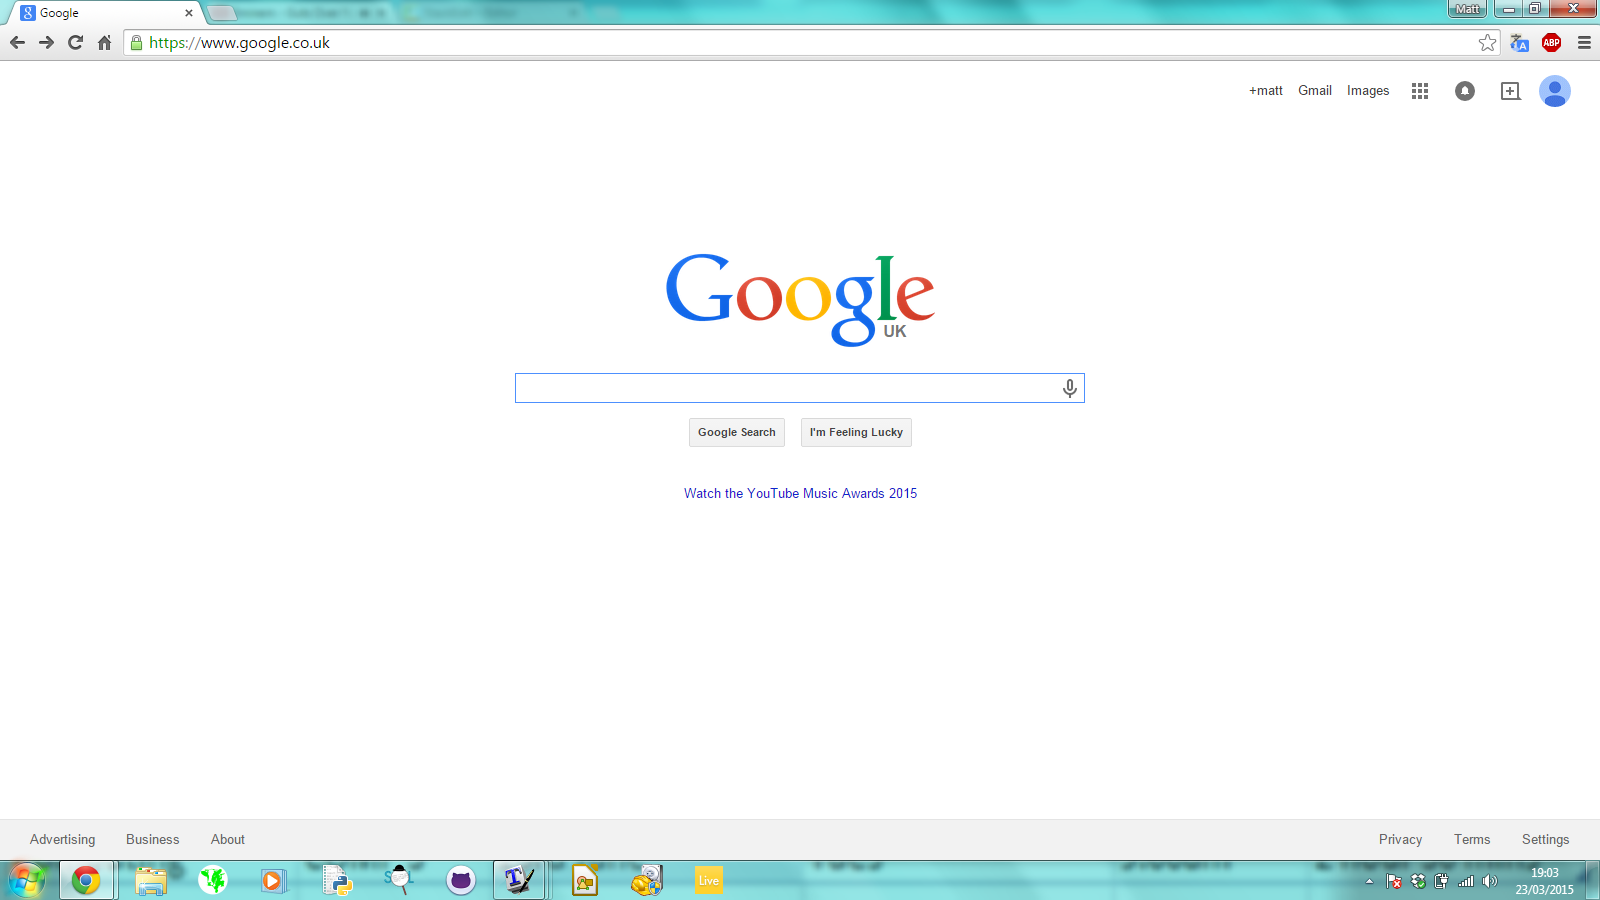
\includegraphics[width=\textwidth]{./ManualImages/download-1.png}

\vspace{5mm}

\textbf{2.} When the web browser has fully loaded, type \newline "https://github.com/mattling9/COMP4Coursework" into the address bar.

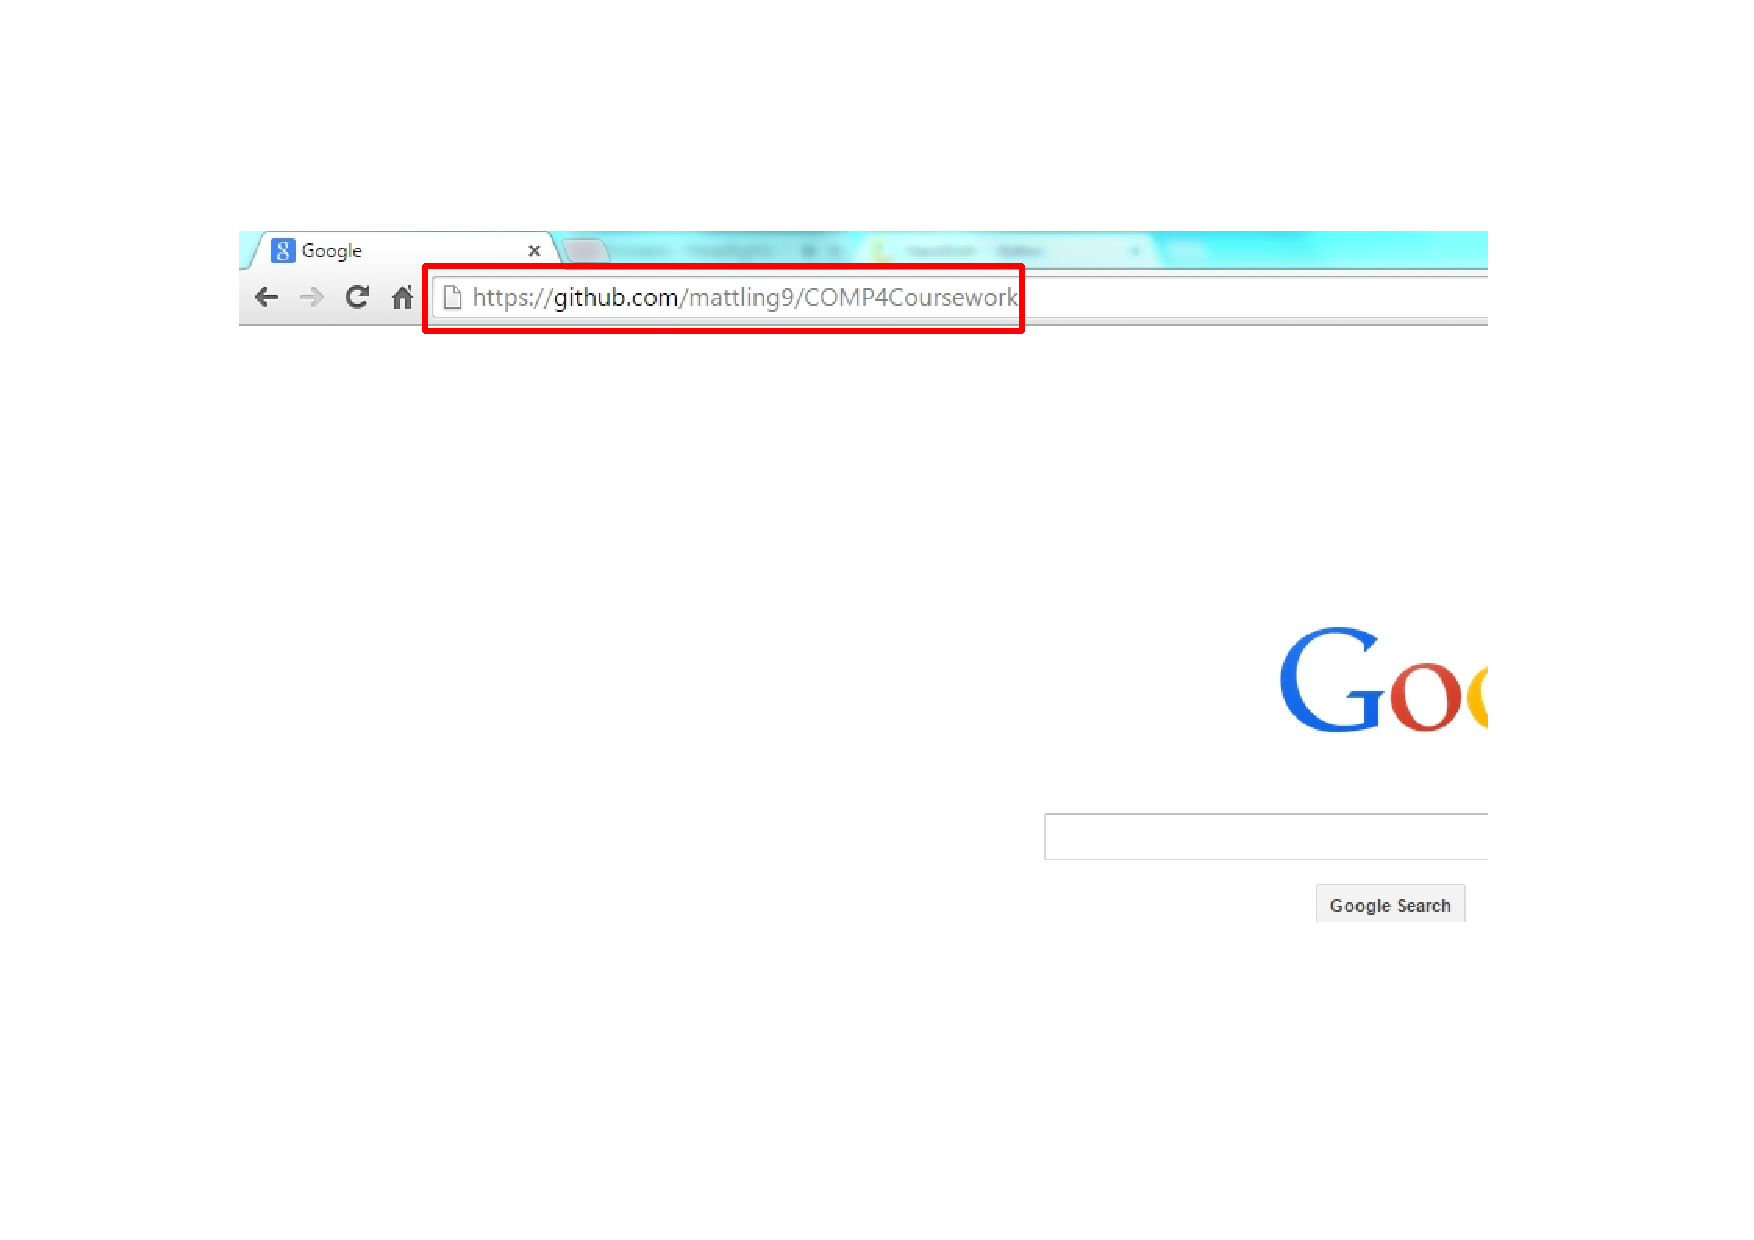
\includegraphics[width=\textwidth]{./ManualImages/download-2.pdf}

\pagebreak

\textbf{3.} Once the page has loaded, click on the 'release' button, this is shown in the diagram below.

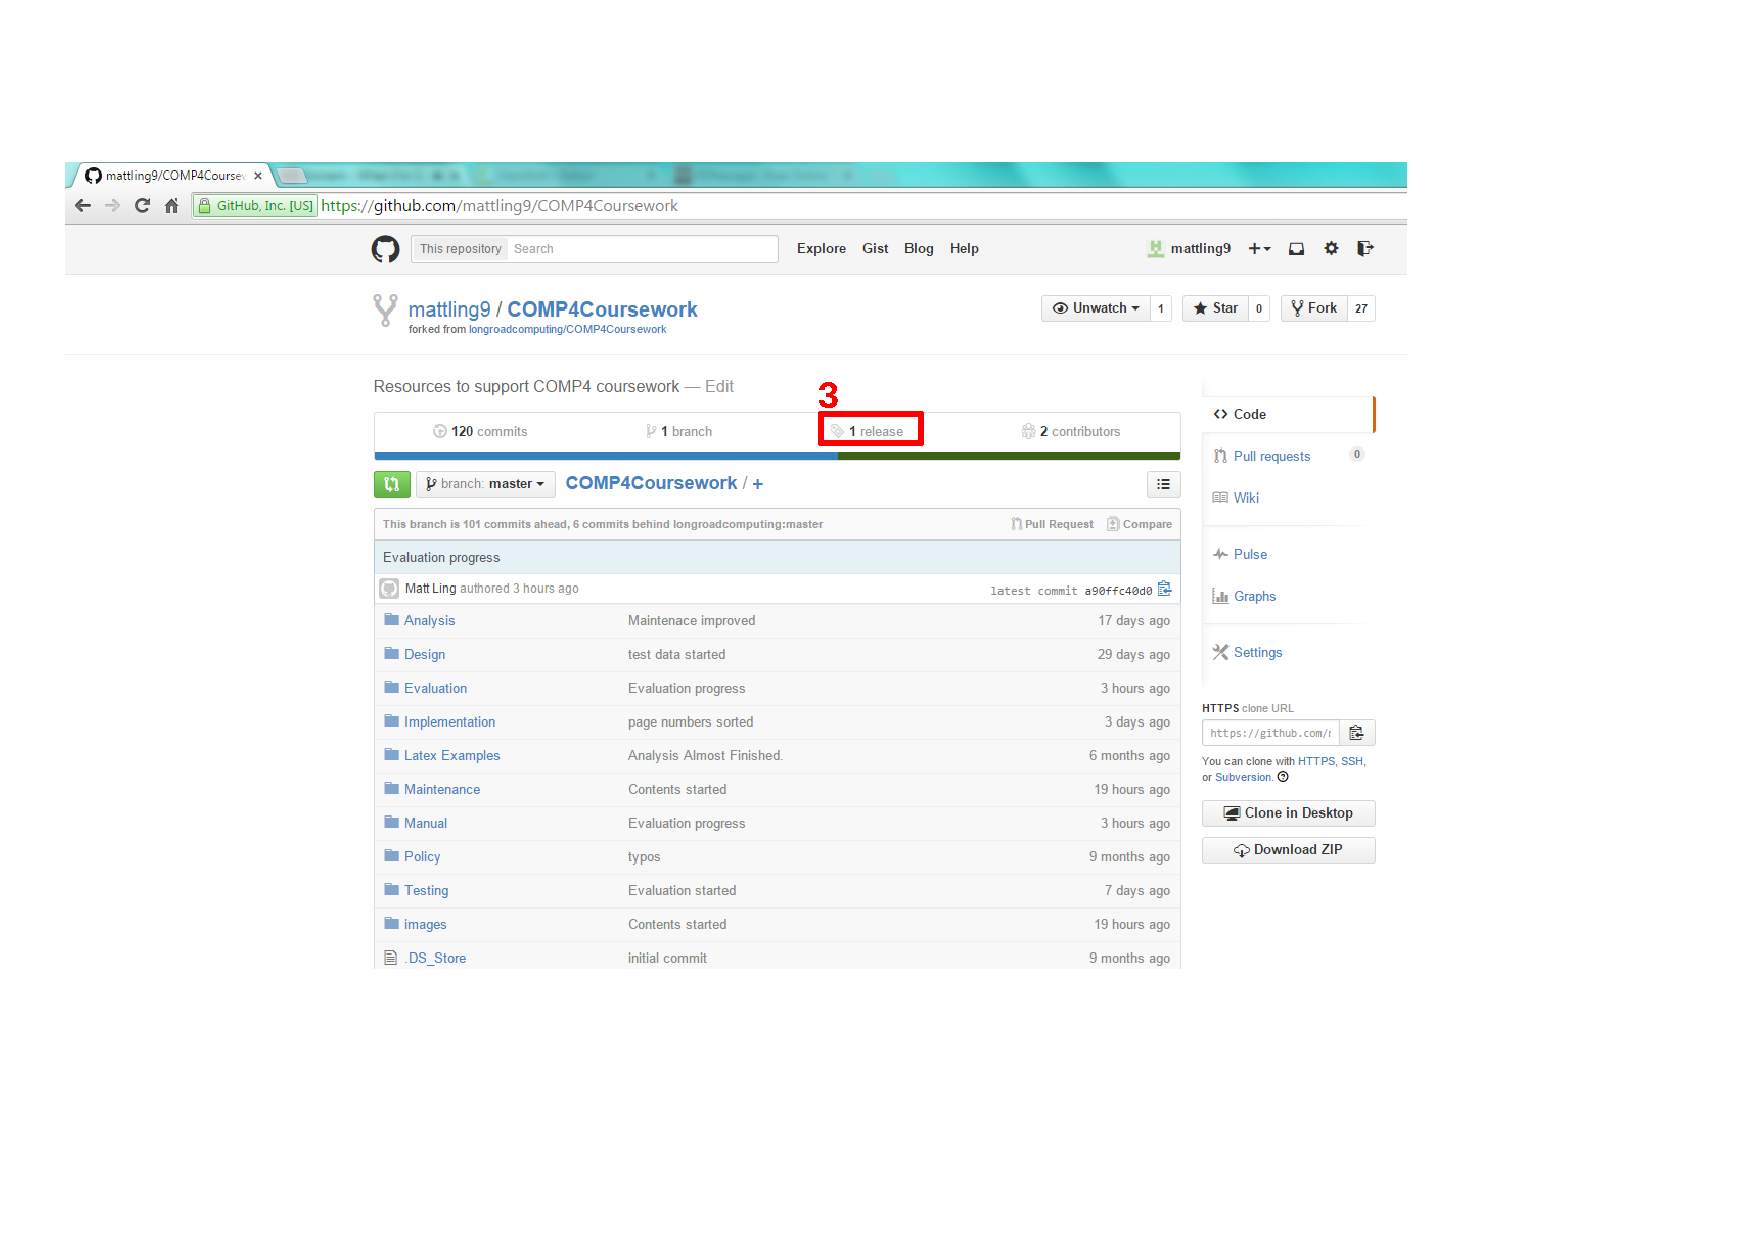
\includegraphics[width=\textwidth]{./ManualImages/download-3.pdf}

\vspace{5mm}

\textbf{4.} Left click on "Beacon.Vets.Stock.Control.msi" under the downloads section. 

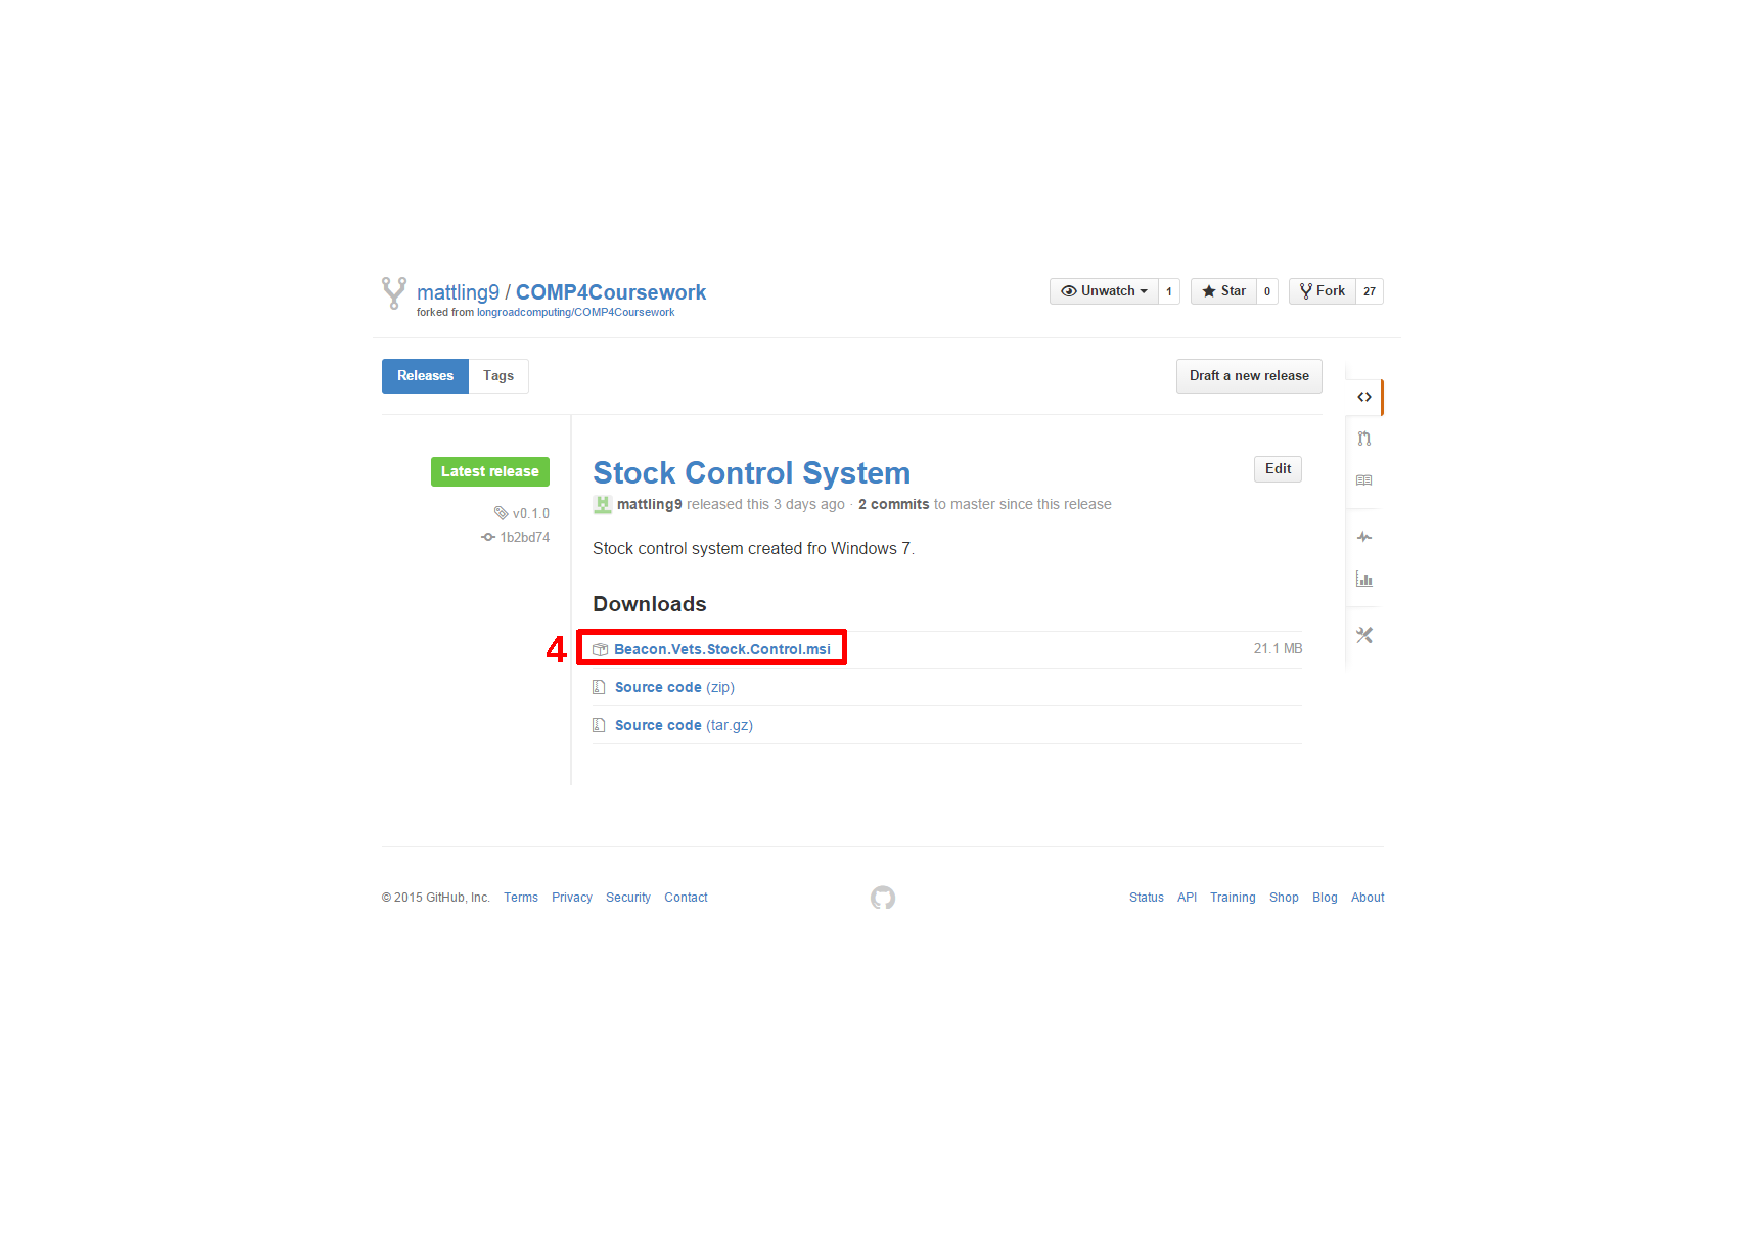
\includegraphics[width=\textwidth]{./ManualImages/download-4.pdf}

\vspace{5mm}

\pagebreak

\textbf{5.} Choose a location to save the installer, in this example, it is saved on the Desktop.

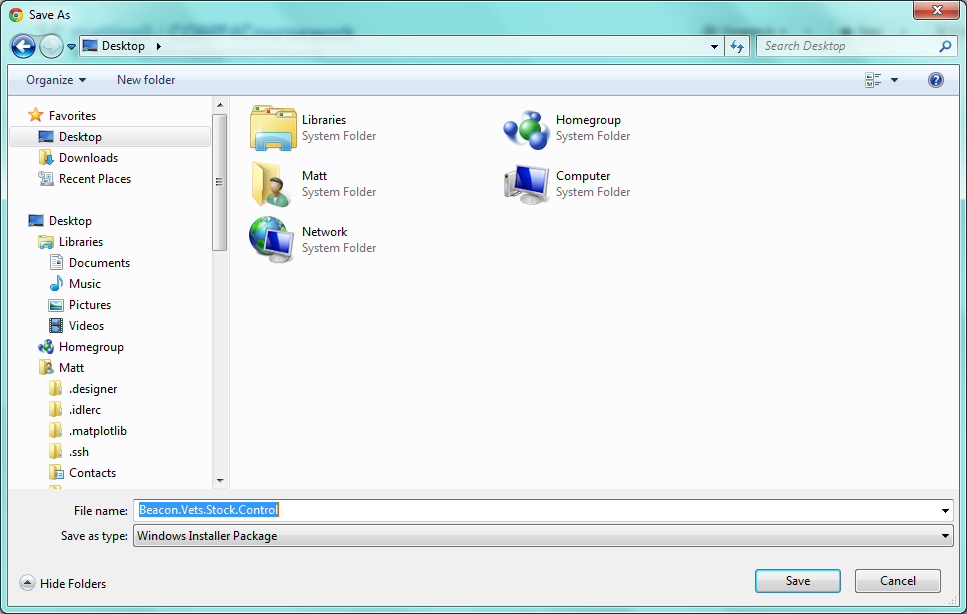
\includegraphics[width=\textwidth]{./ManualImages/download-5.png}

\vspace{5mm}

\textbf{6.} Click the save button.

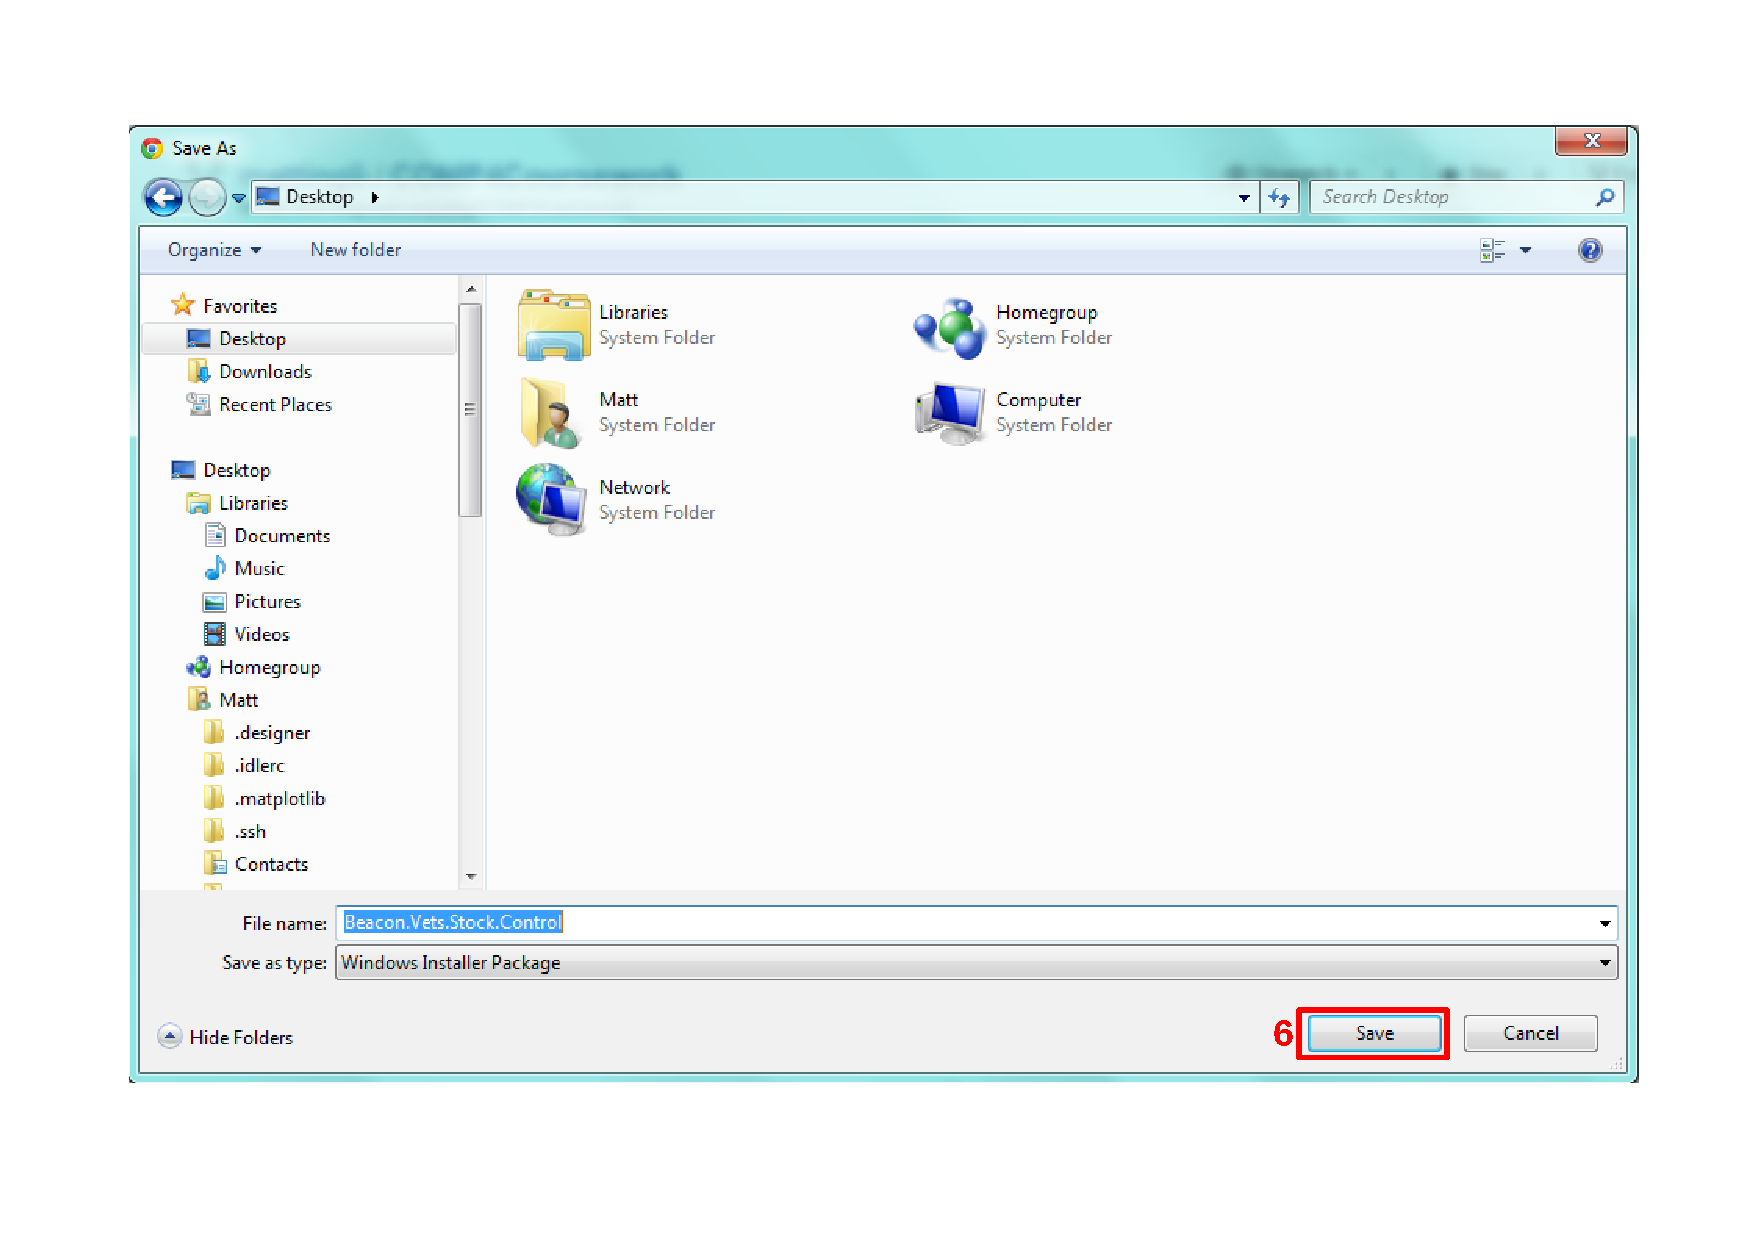
\includegraphics[width=\textwidth]{./ManualImages/download-6.pdf}

\pagebreak

\vspace{5mm}

Alternatively, if you do not have Internet Access, the instructions below explain how to access the installer from a USB flash device or a CD-R.

\textbf{1.} Click on the Start Button in the bottom left hand corner of the screen.

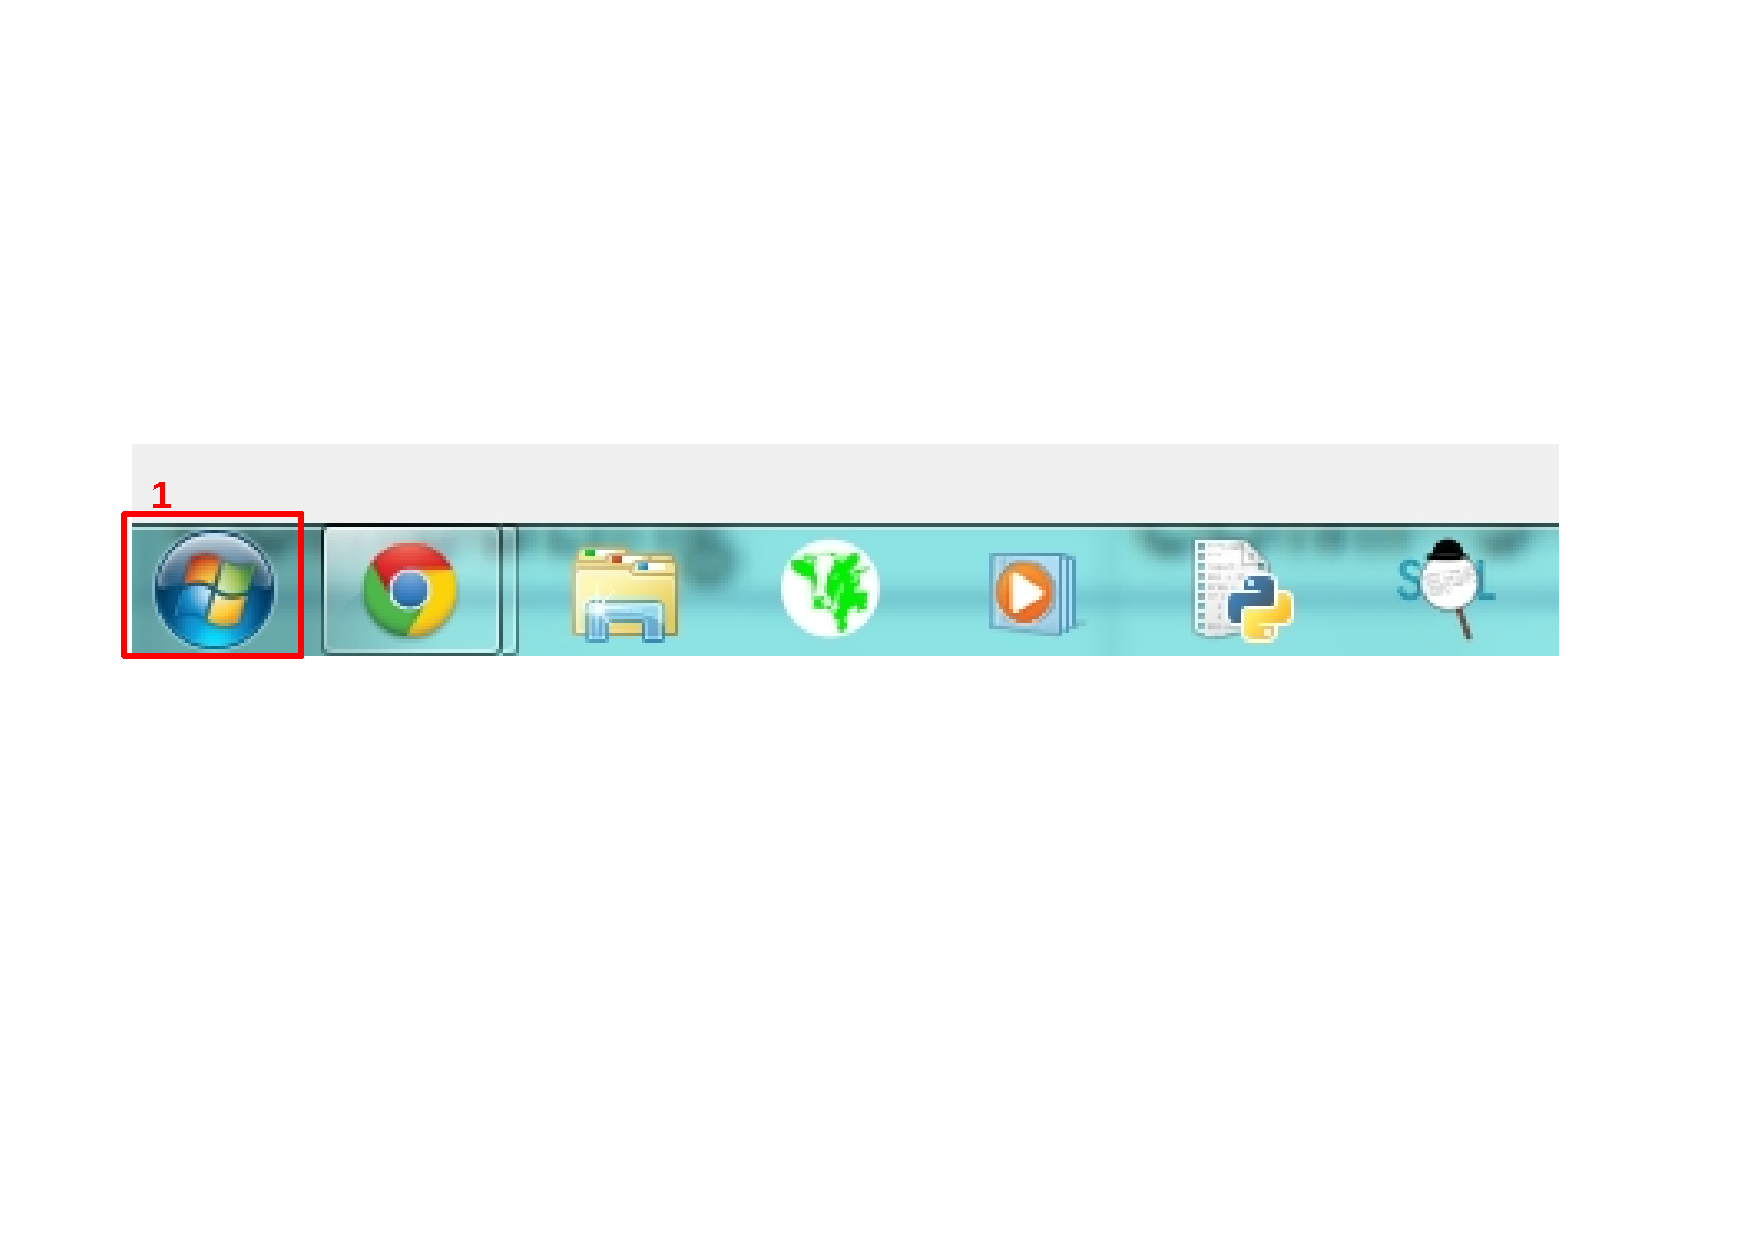
\includegraphics[width=\textwidth]{./ManualImages/download-usb-1.pdf}

\vspace{5mm}

\textbf{2.} Click on 'Computer' on the right hand side of the start menu.

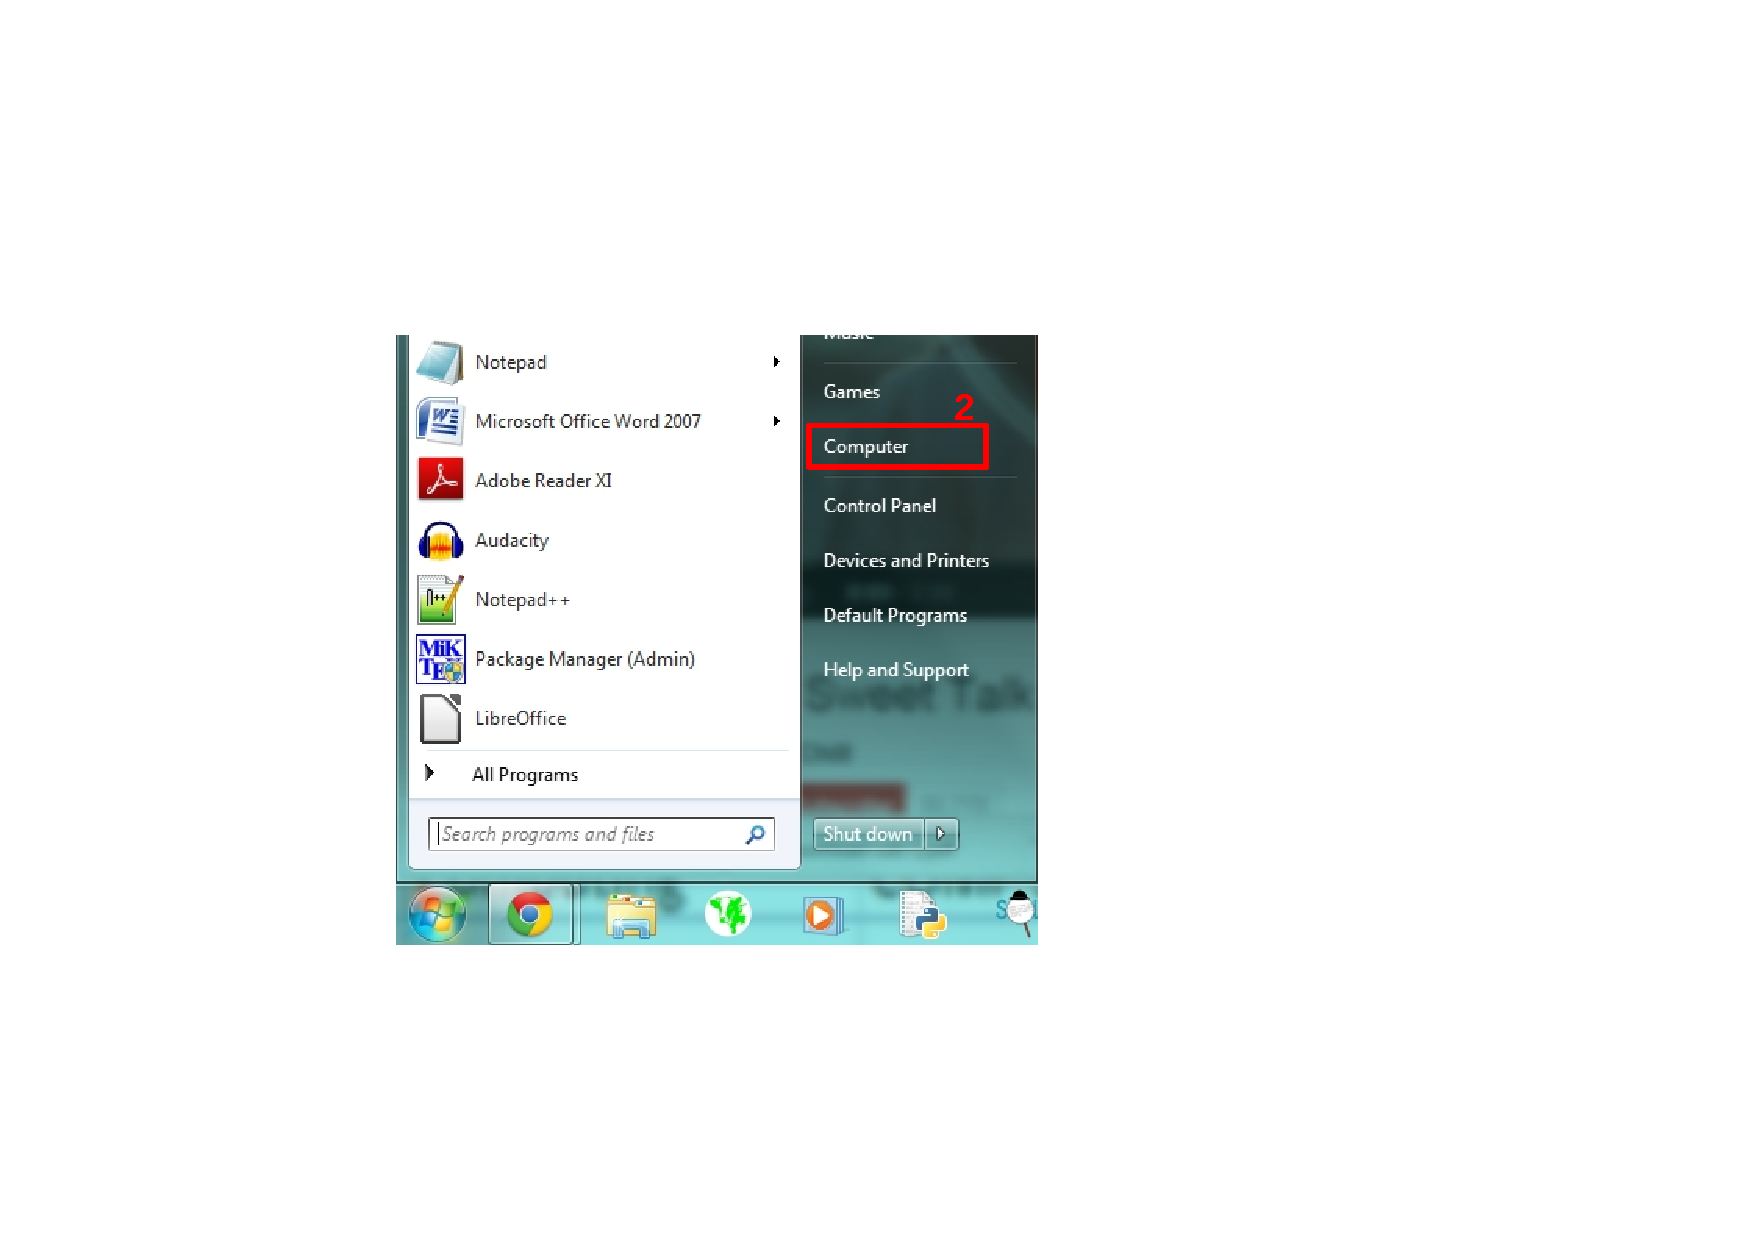
\includegraphics[width=\textwidth]{./ManualImages/download-usb-2.pdf}

\pagebreak

\vspace{5mm}
\textbf{3.} Insert the CD-R or the USB device. it should display under the 'Devices with Removable Storage' section momentarily. 

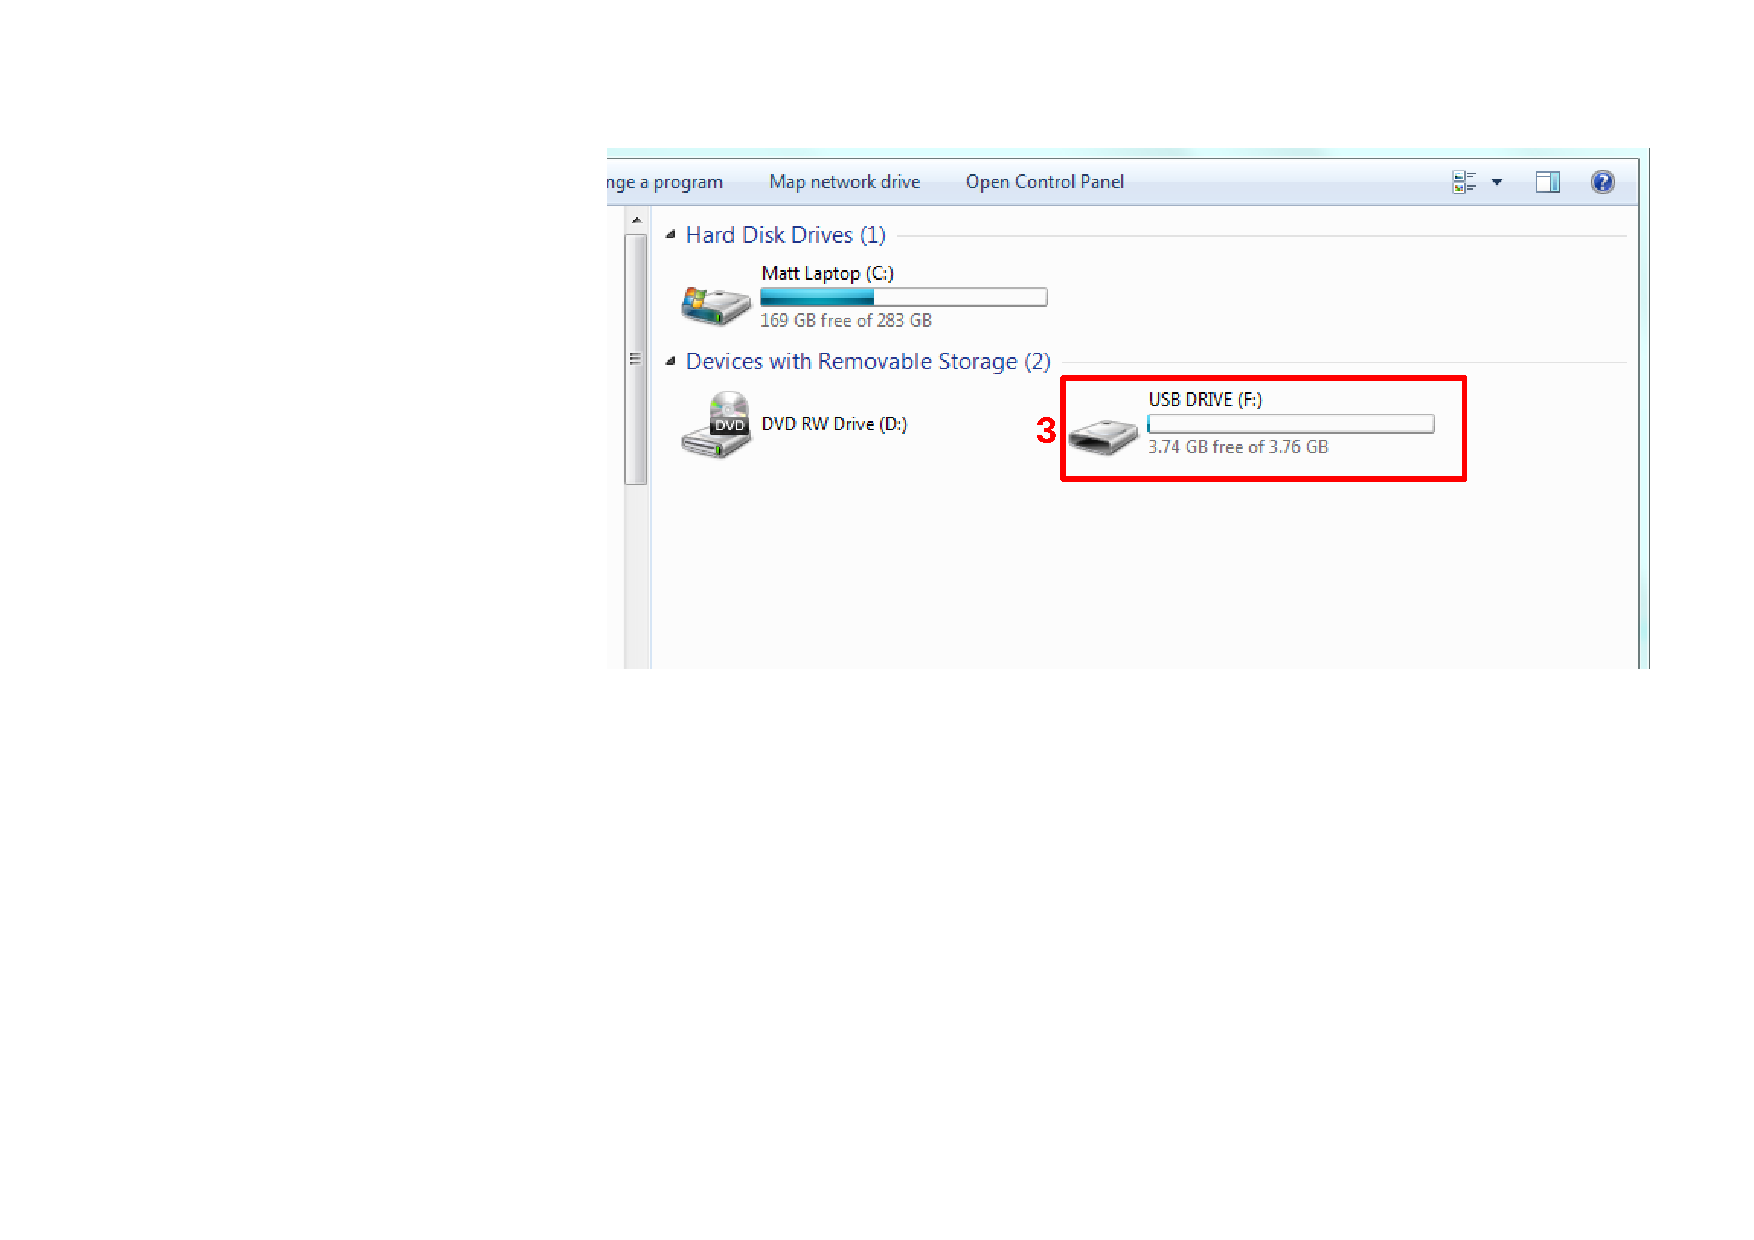
\includegraphics[width=\textwidth]{./ManualImages/download-usb-3.pdf}

\vspace{5mm}
\textbf{4.} Double left click on the USB Device or your CD-R.

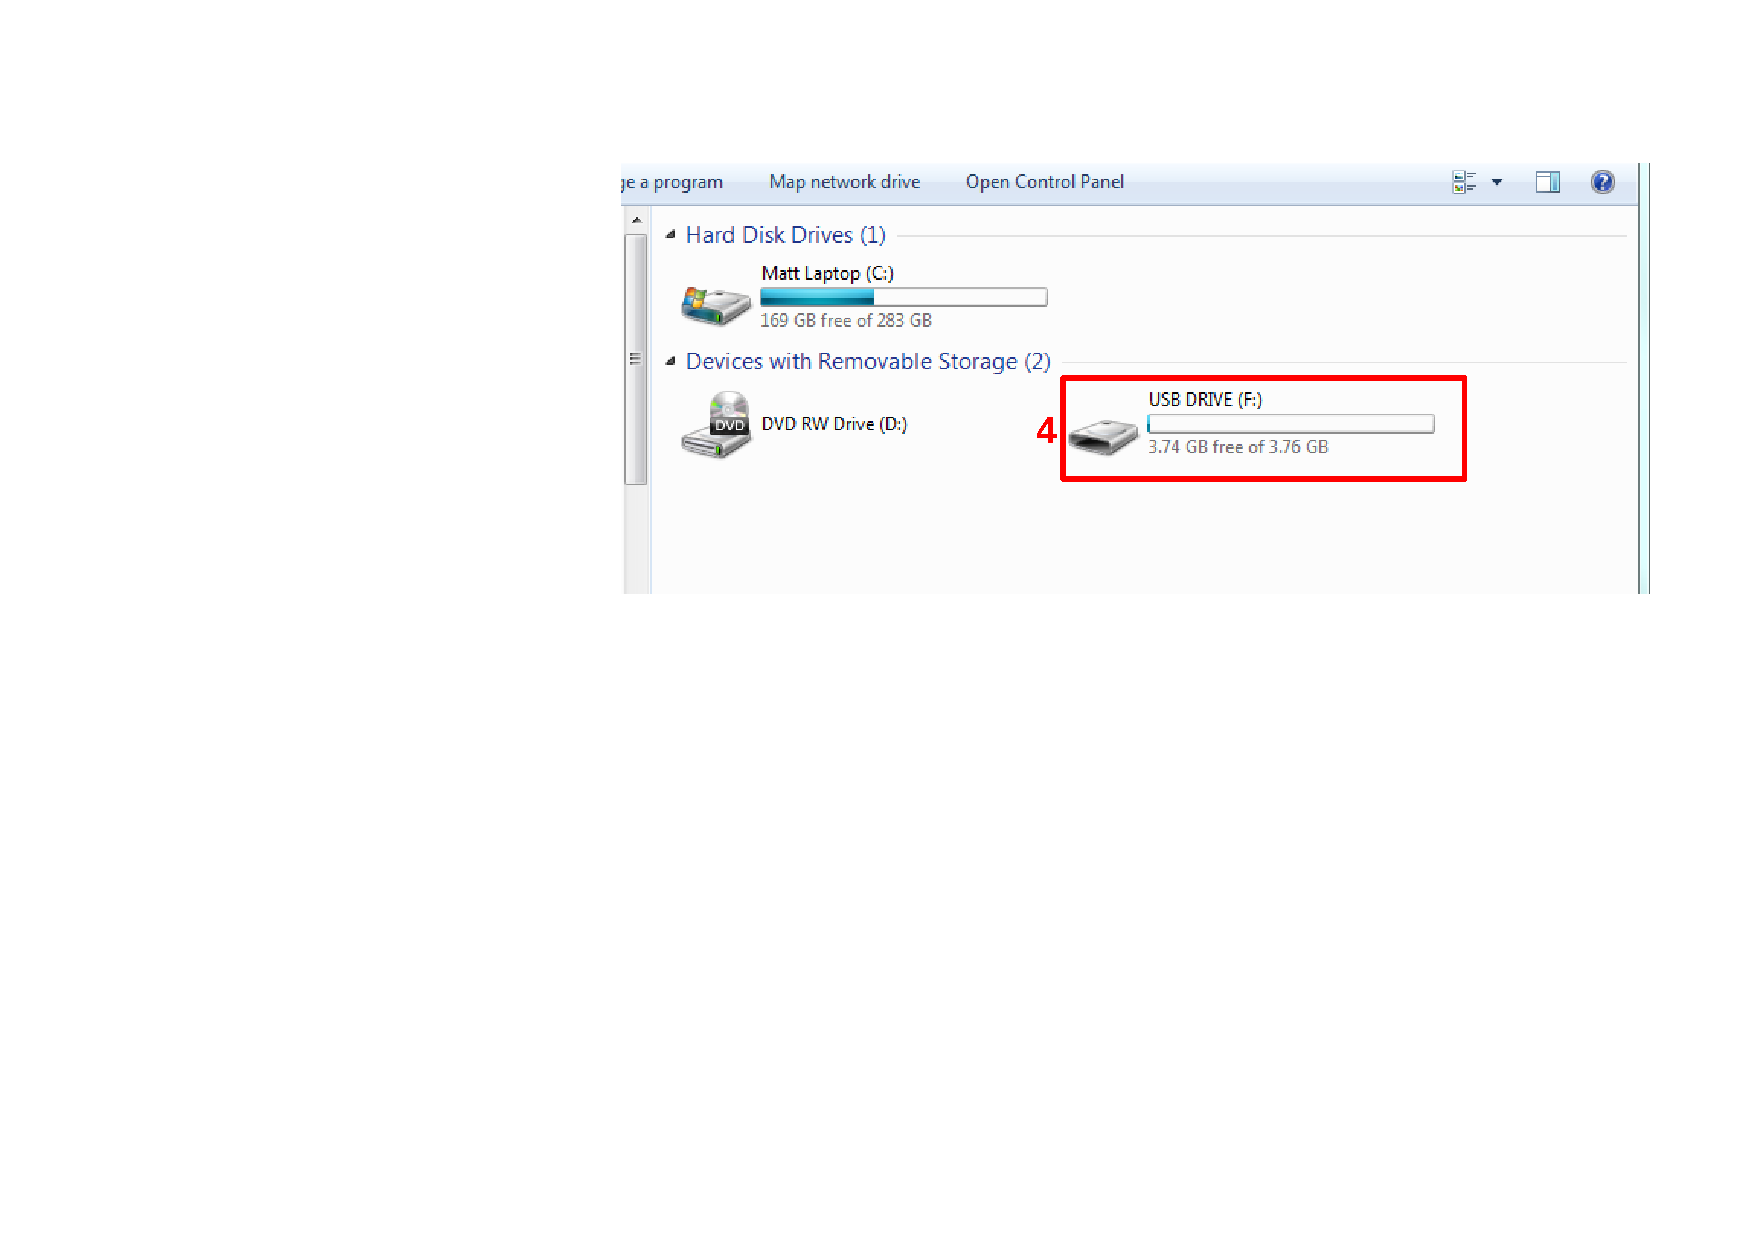
\includegraphics[width=\textwidth]{./ManualImages/download-usb-4.pdf}

\vspace{5mm}
\textbf{5.} Locate the "Beacon.Vets.Stock.Control.msi" file.

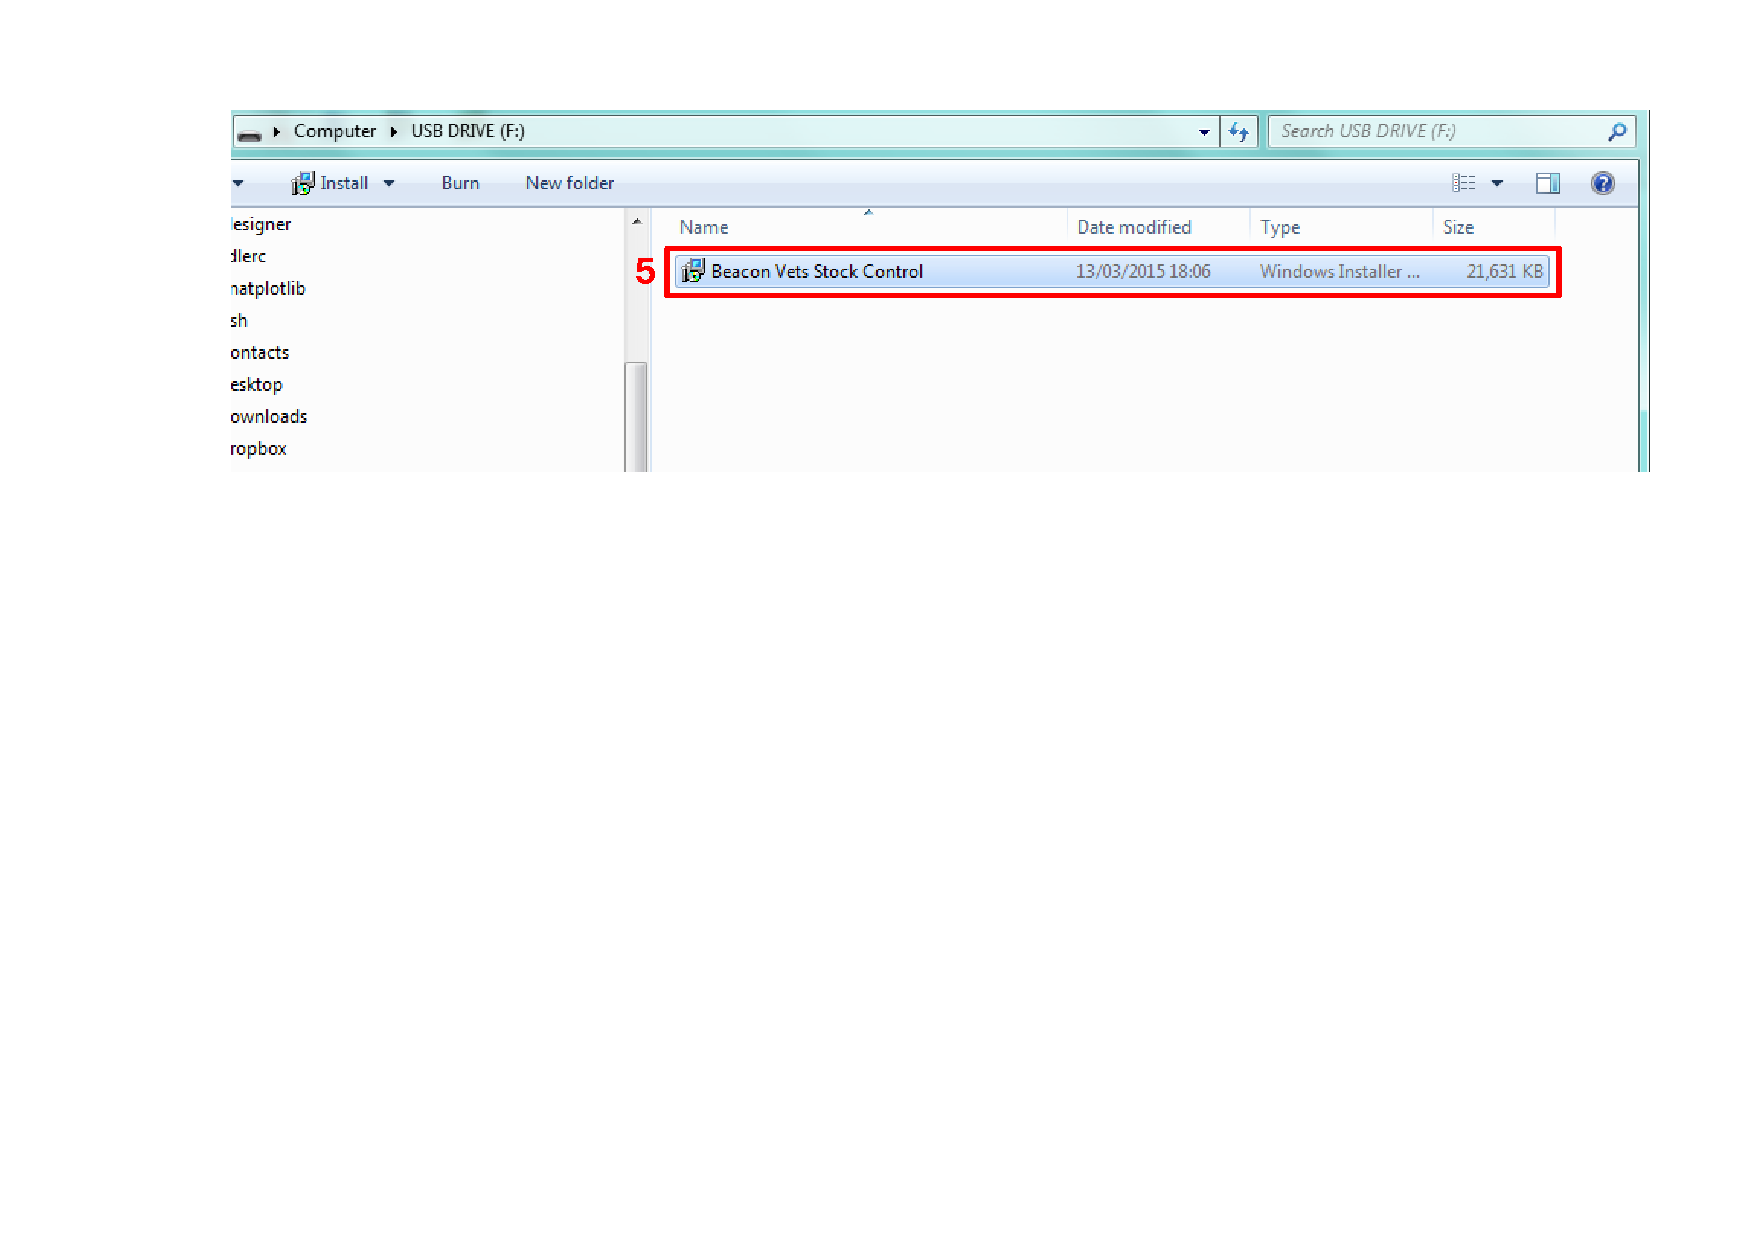
\includegraphics[width=\textwidth]{./ManualImages/download-usb-5.pdf}

\vspace{5mm}
\textbf{6.} When the installer needs to be run, double left click on the file.


\vspace{5mm}

Once you have either downloaded the installer or found the installer stored on a USB or CD-R, follow the instructions below to install the system.

\textbf{1.} Open Windows explorer, by default, it can be found in the Taskbar.

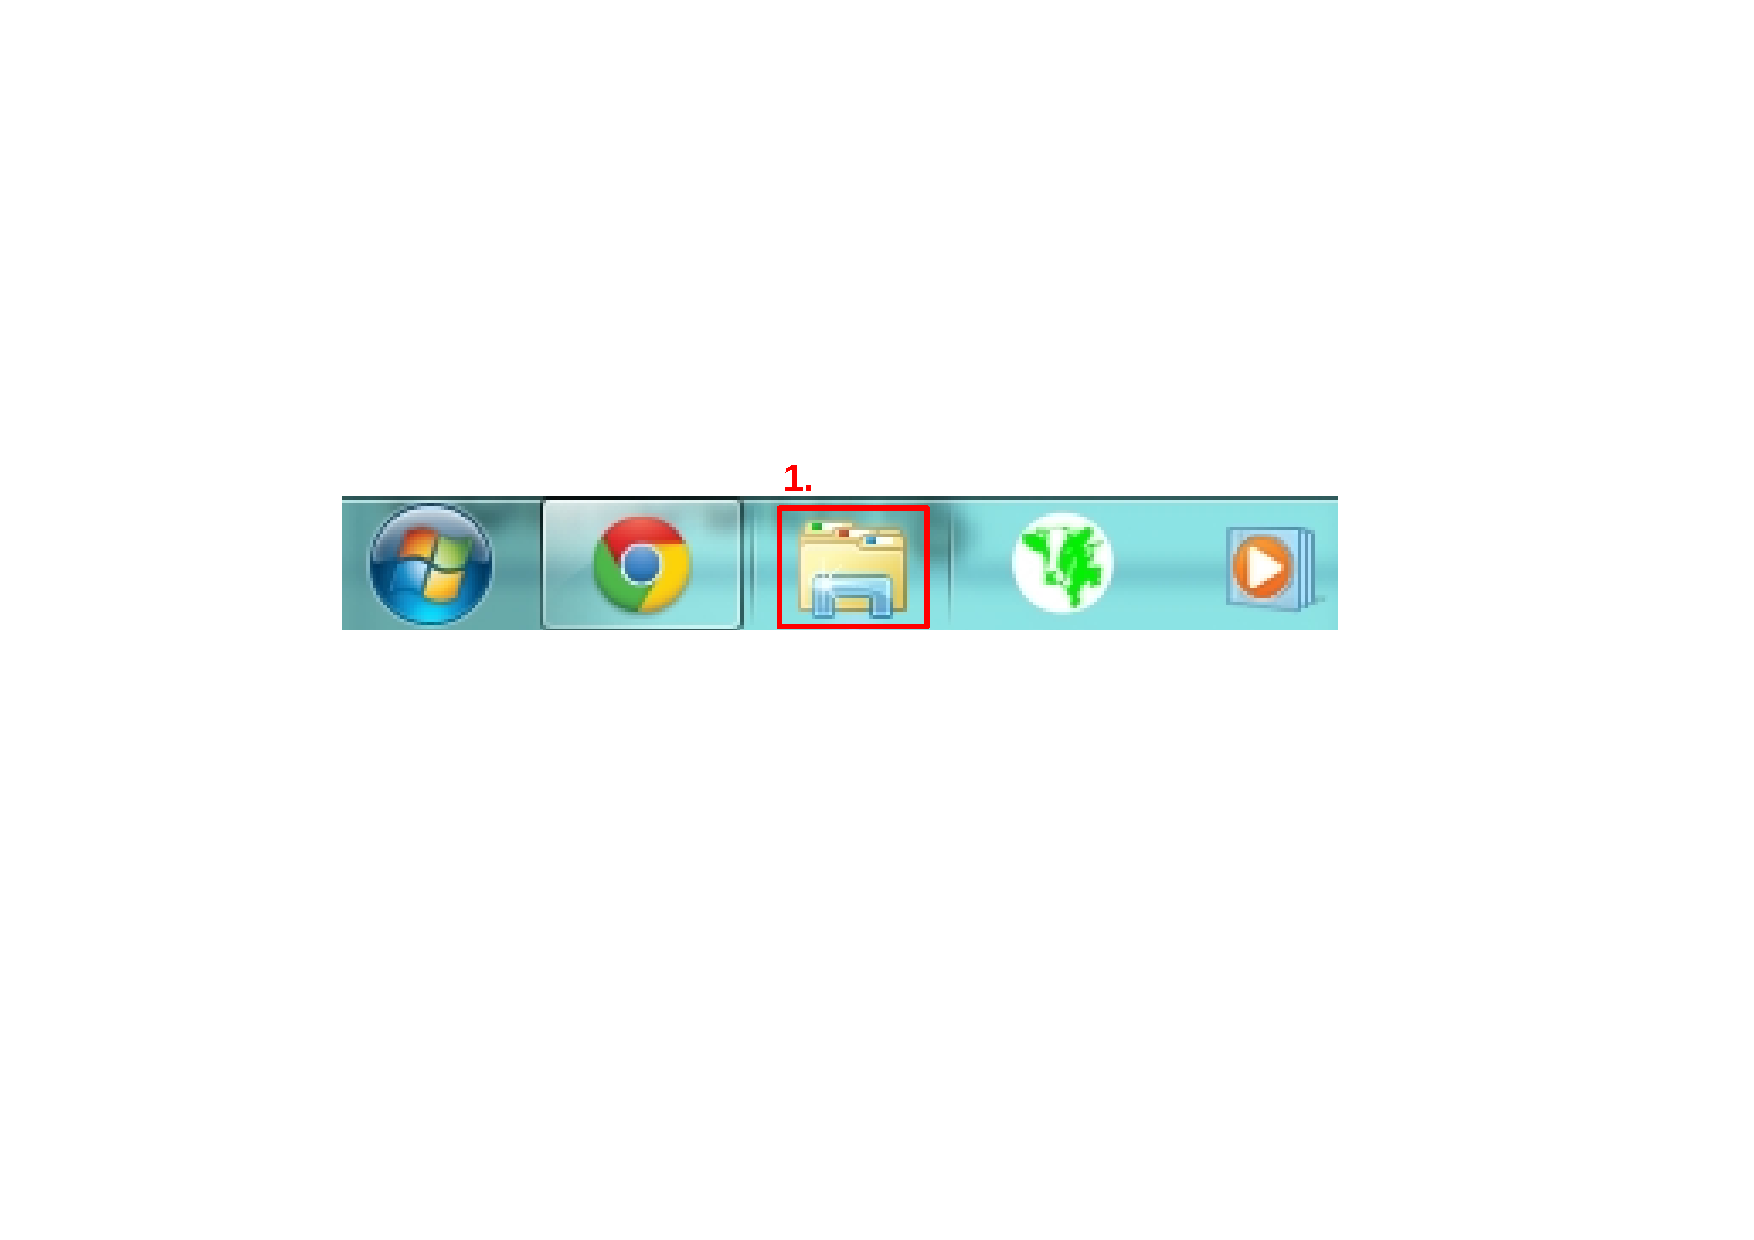
\includegraphics[width=\textwidth]{./ManualImages/explorer-1.pdf}

\textbf{2.} Create a New Folder in the location in which you want to store the system. in this example it is being created on the Desktop.

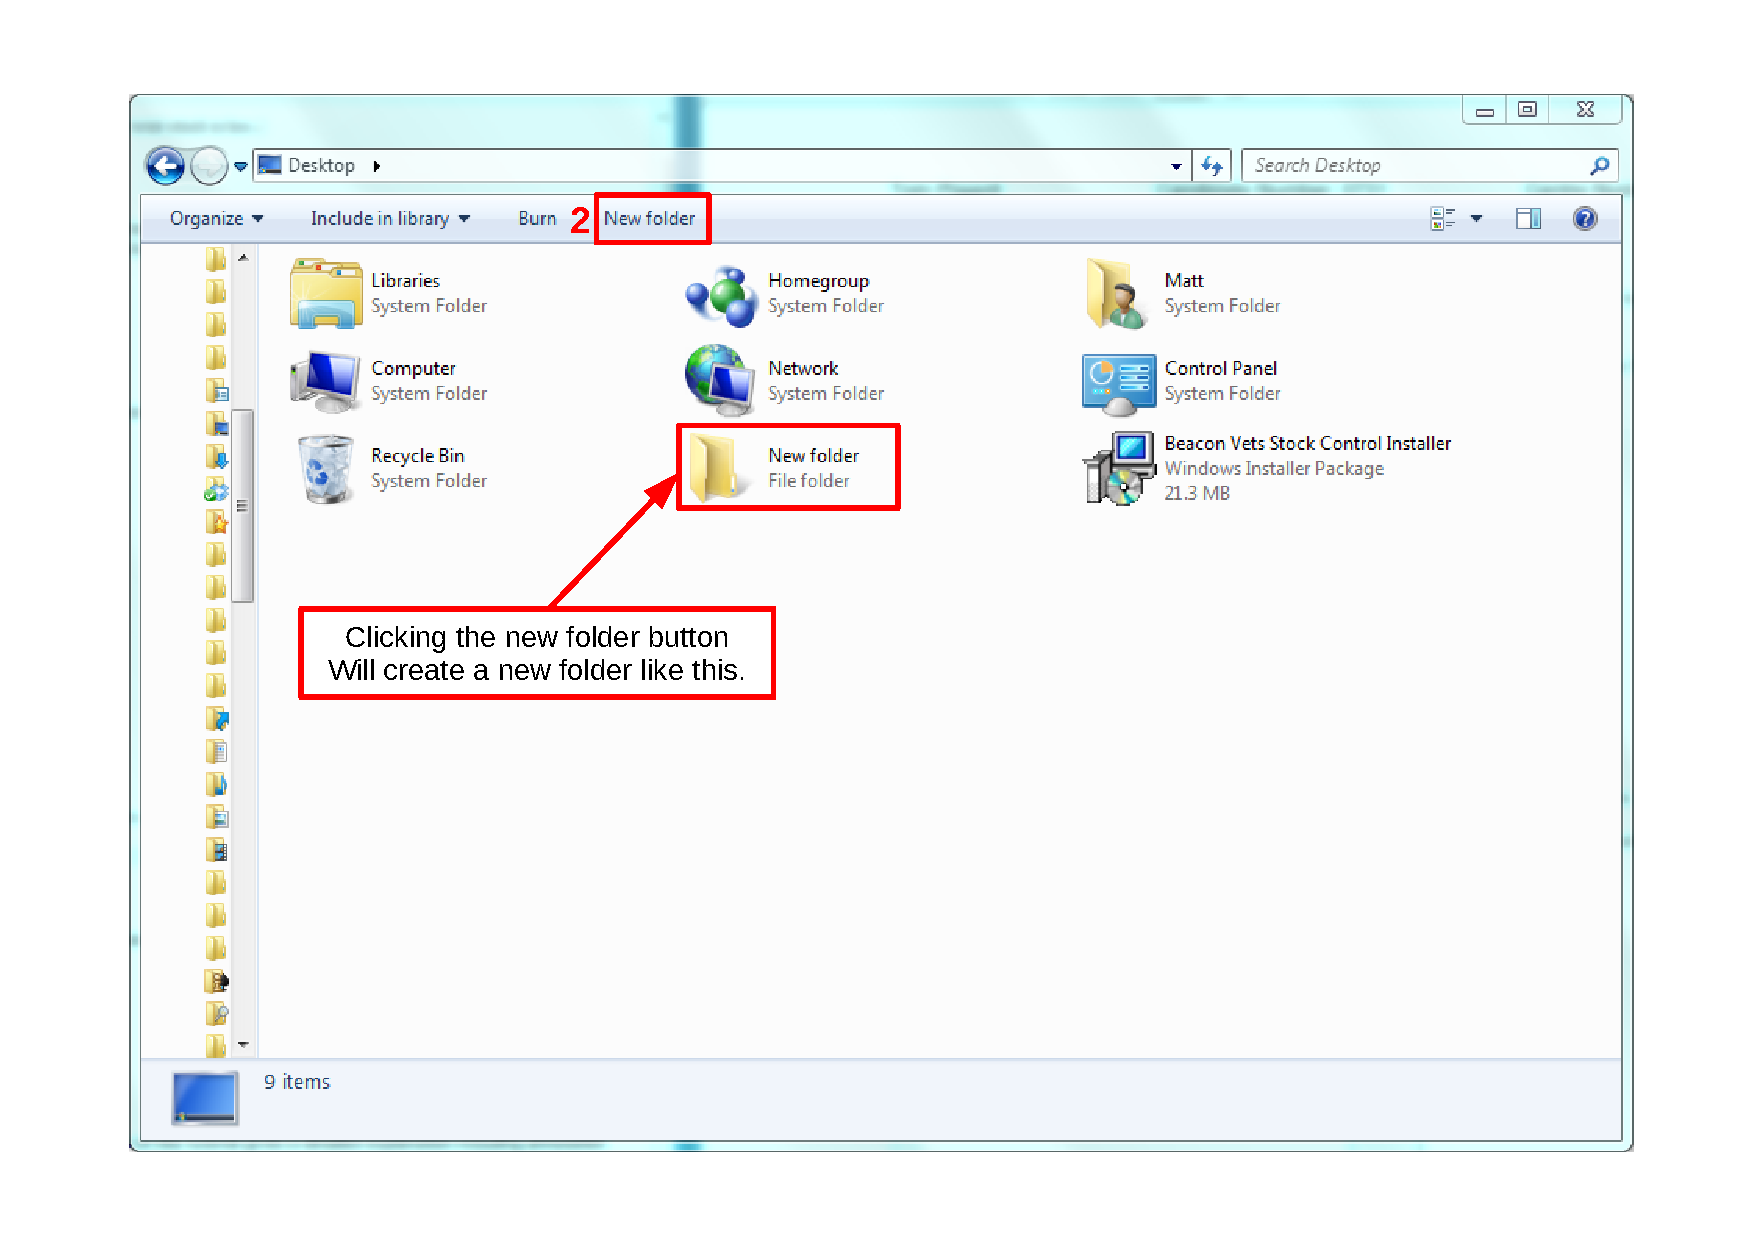
\includegraphics[width=\textwidth]{./ManualImages/install-1.pdf}

\pagebreak

\textbf{3.} Rename the folder to `Stock Control System'. This can be done by right clicking the folder and selecting `rename' from the drop down menu.

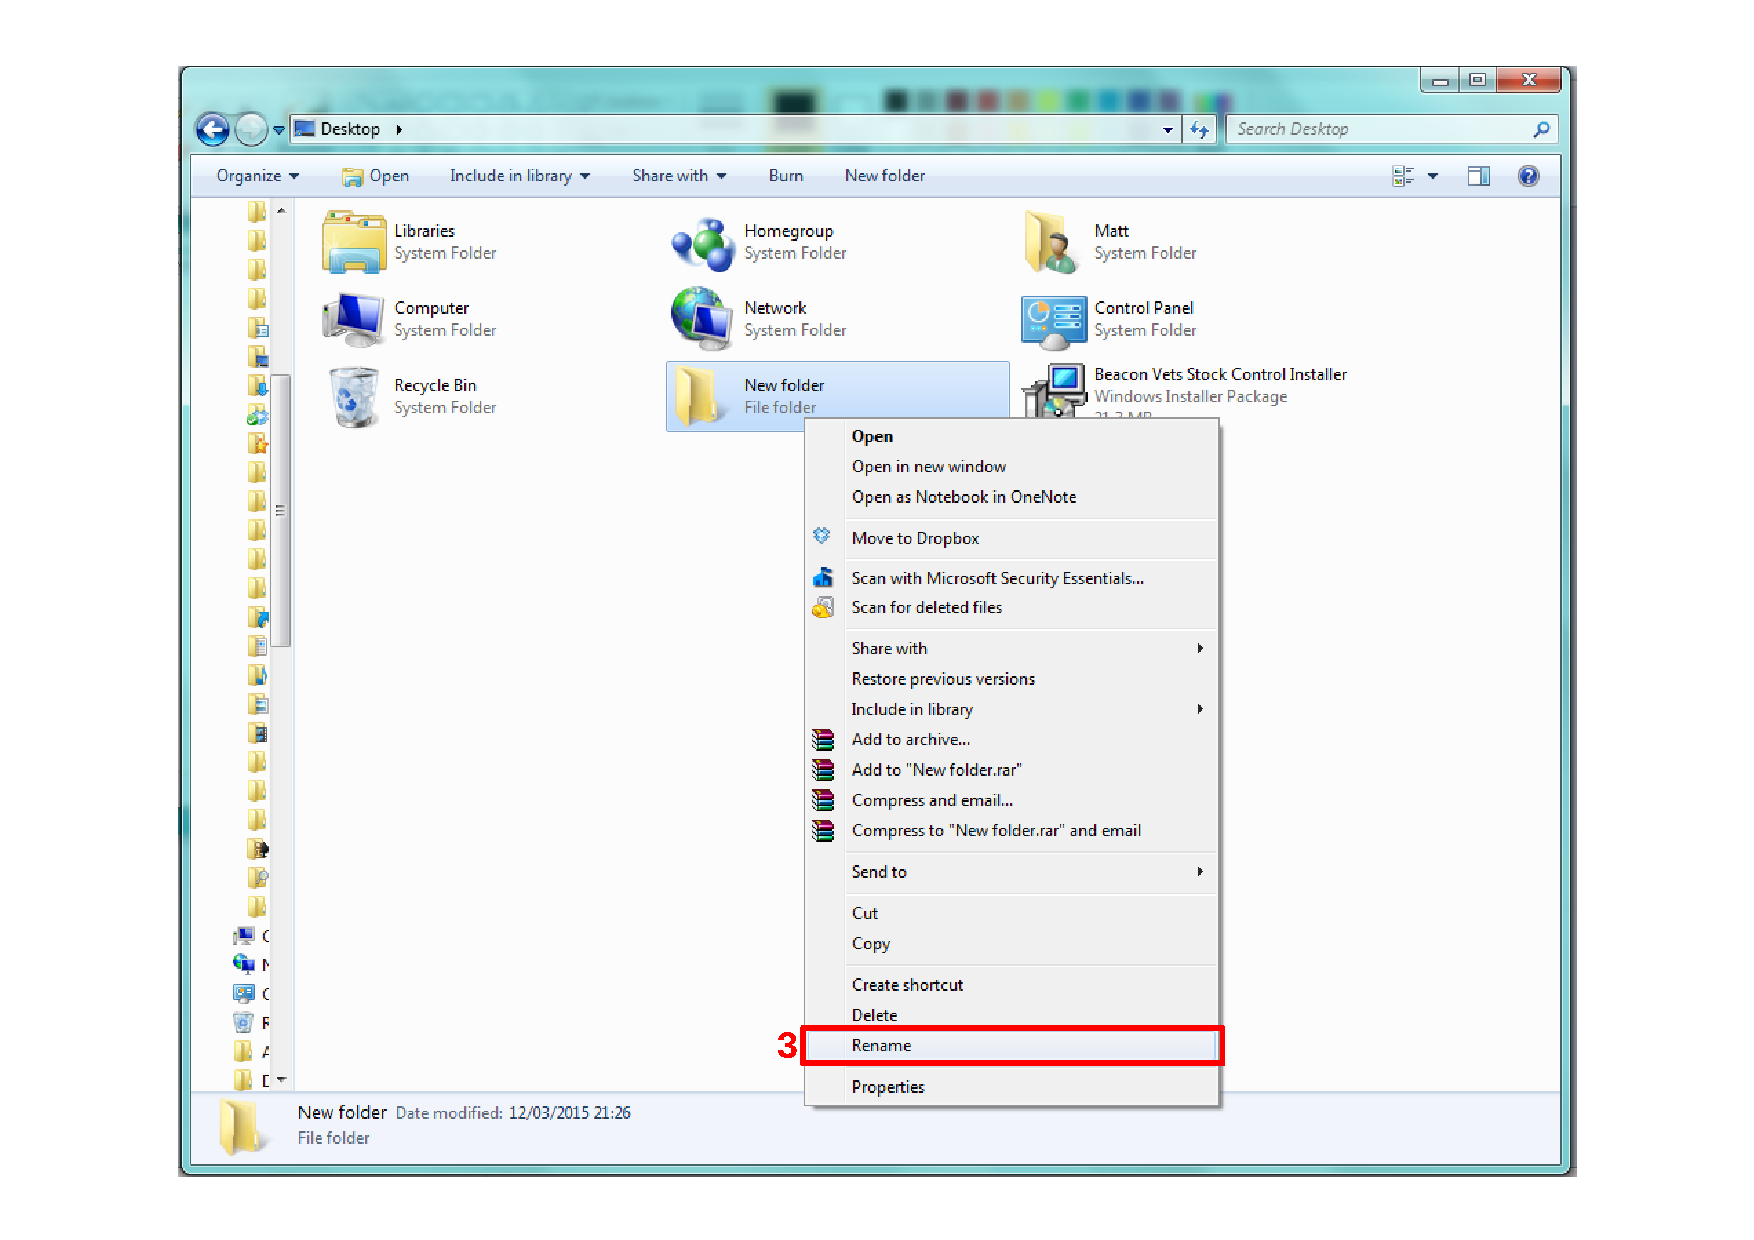
\includegraphics[width=\textwidth]{./ManualImages/install-2.pdf}

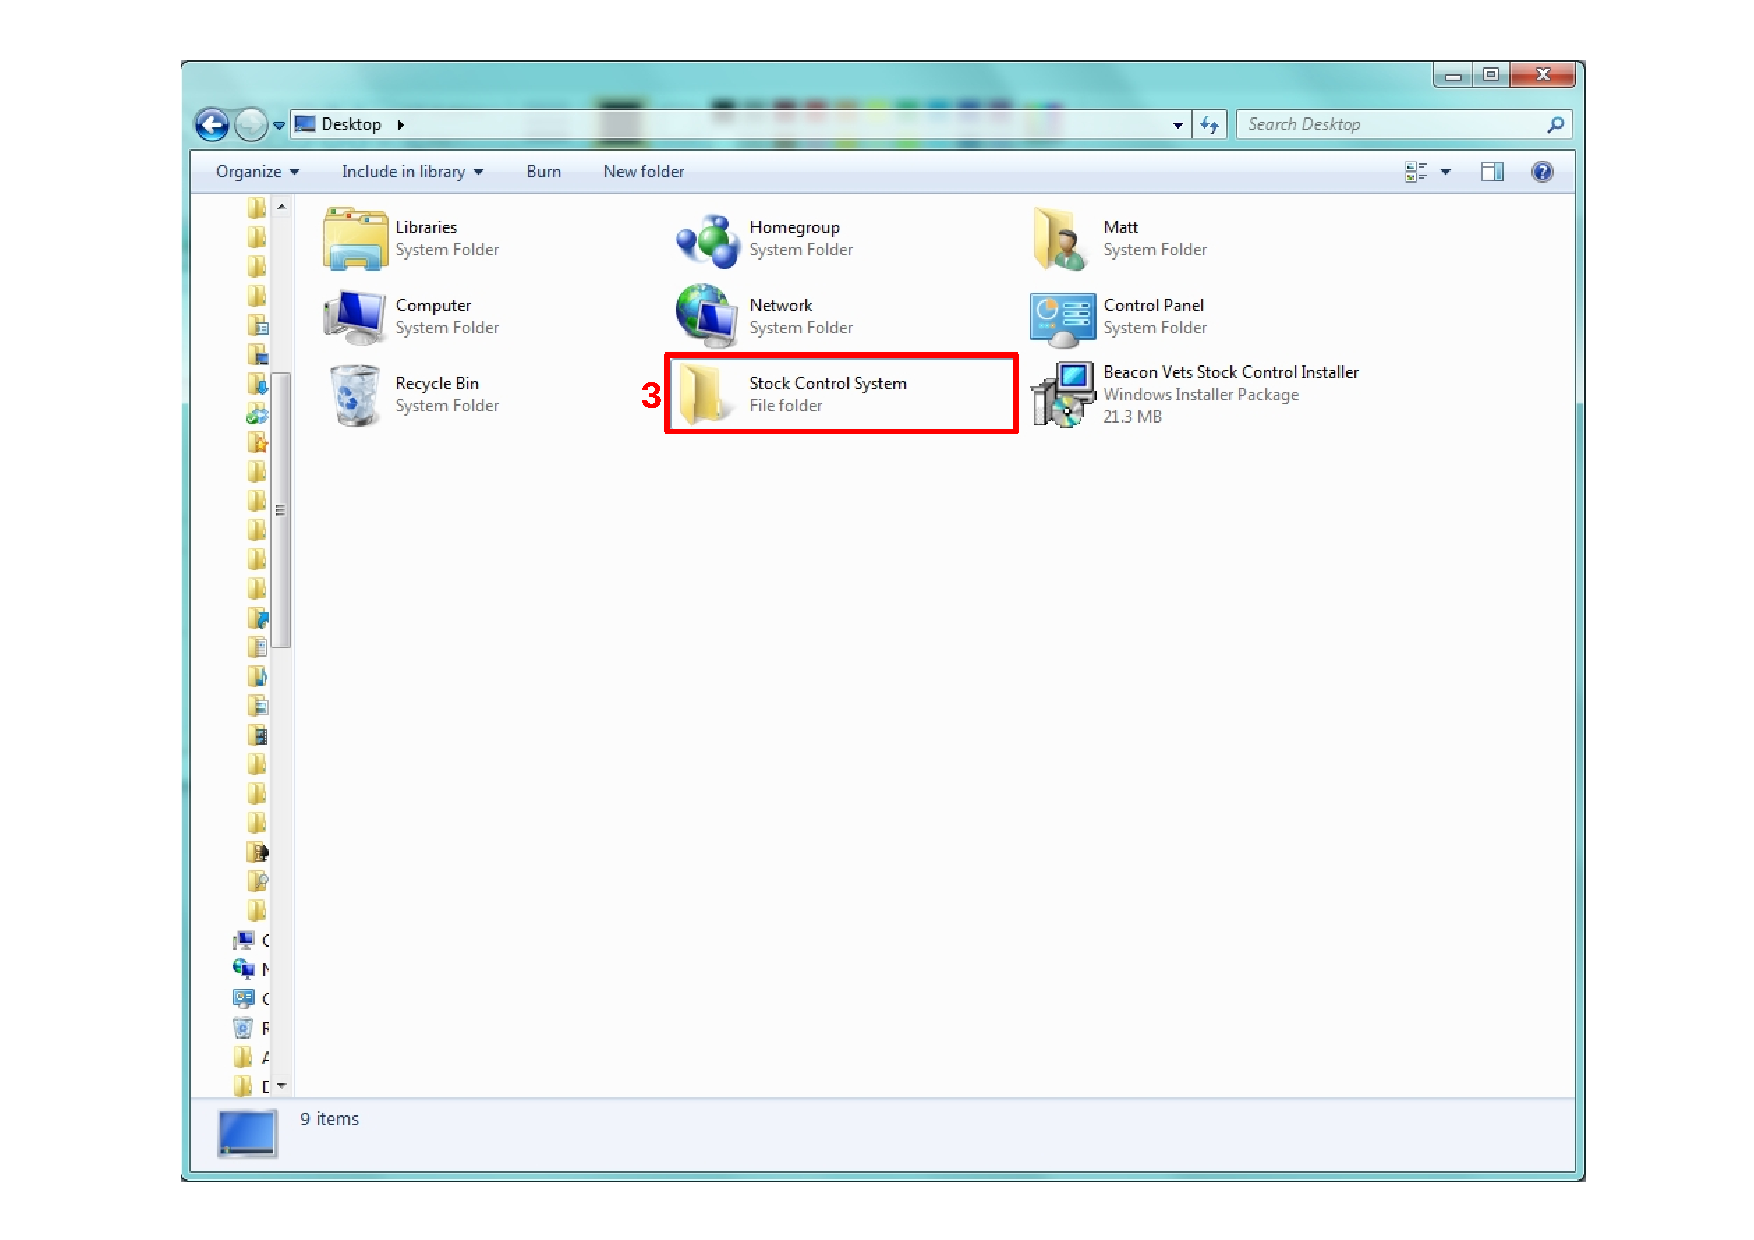
\includegraphics[width=\textwidth]{./ManualImages/install-3.pdf}

\pagebreak

\textbf{4.} Locate the `Beacon Vets Stock Control Installer'. In this case, the installer was placed on the desktop. For instructions on how to get the installer, go to page \pageref{fig:System Installation} of the user manual.

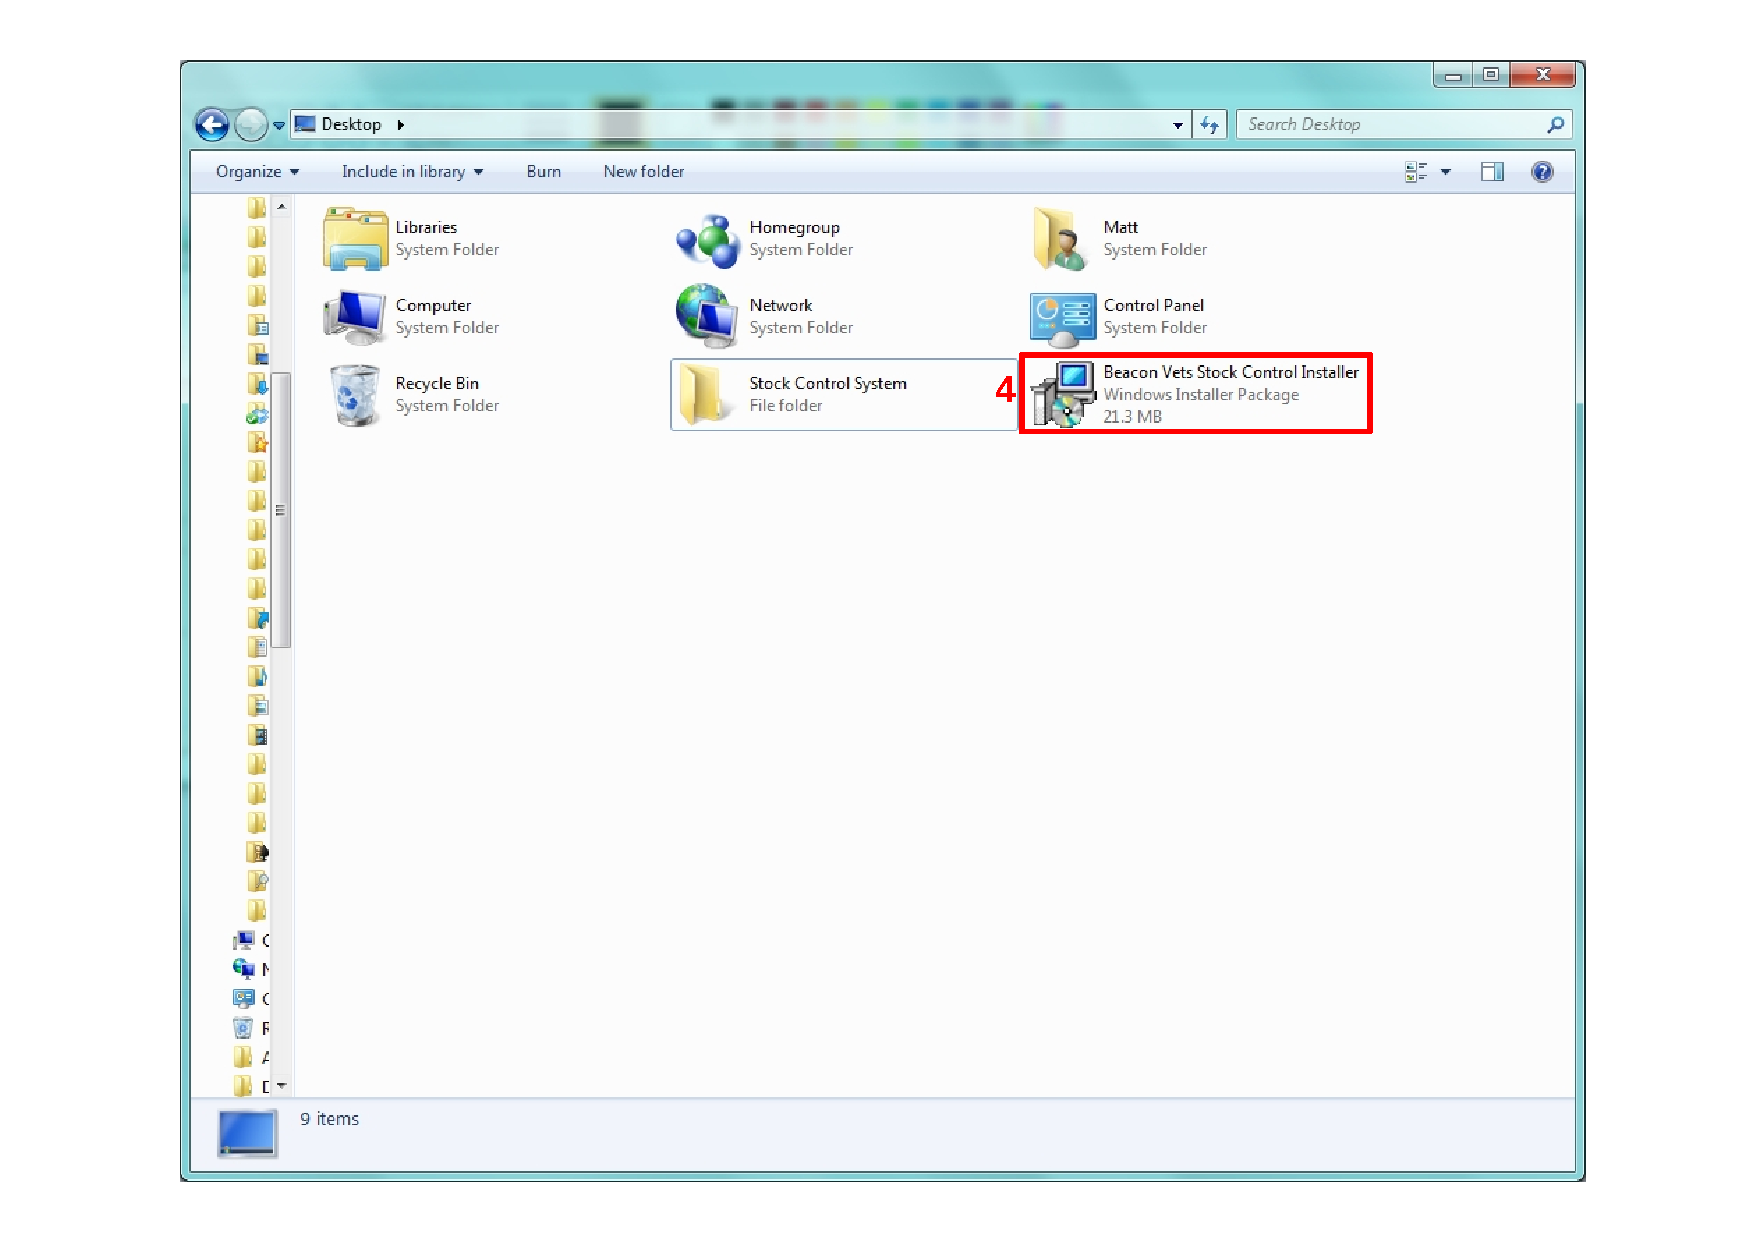
\includegraphics[width=\textwidth]{./ManualImages/install-4.pdf}

\pagebreak

\textbf{5.} Double left click on the `Beacon Vets Stock Control Installer'. You shall be presented with the following window:

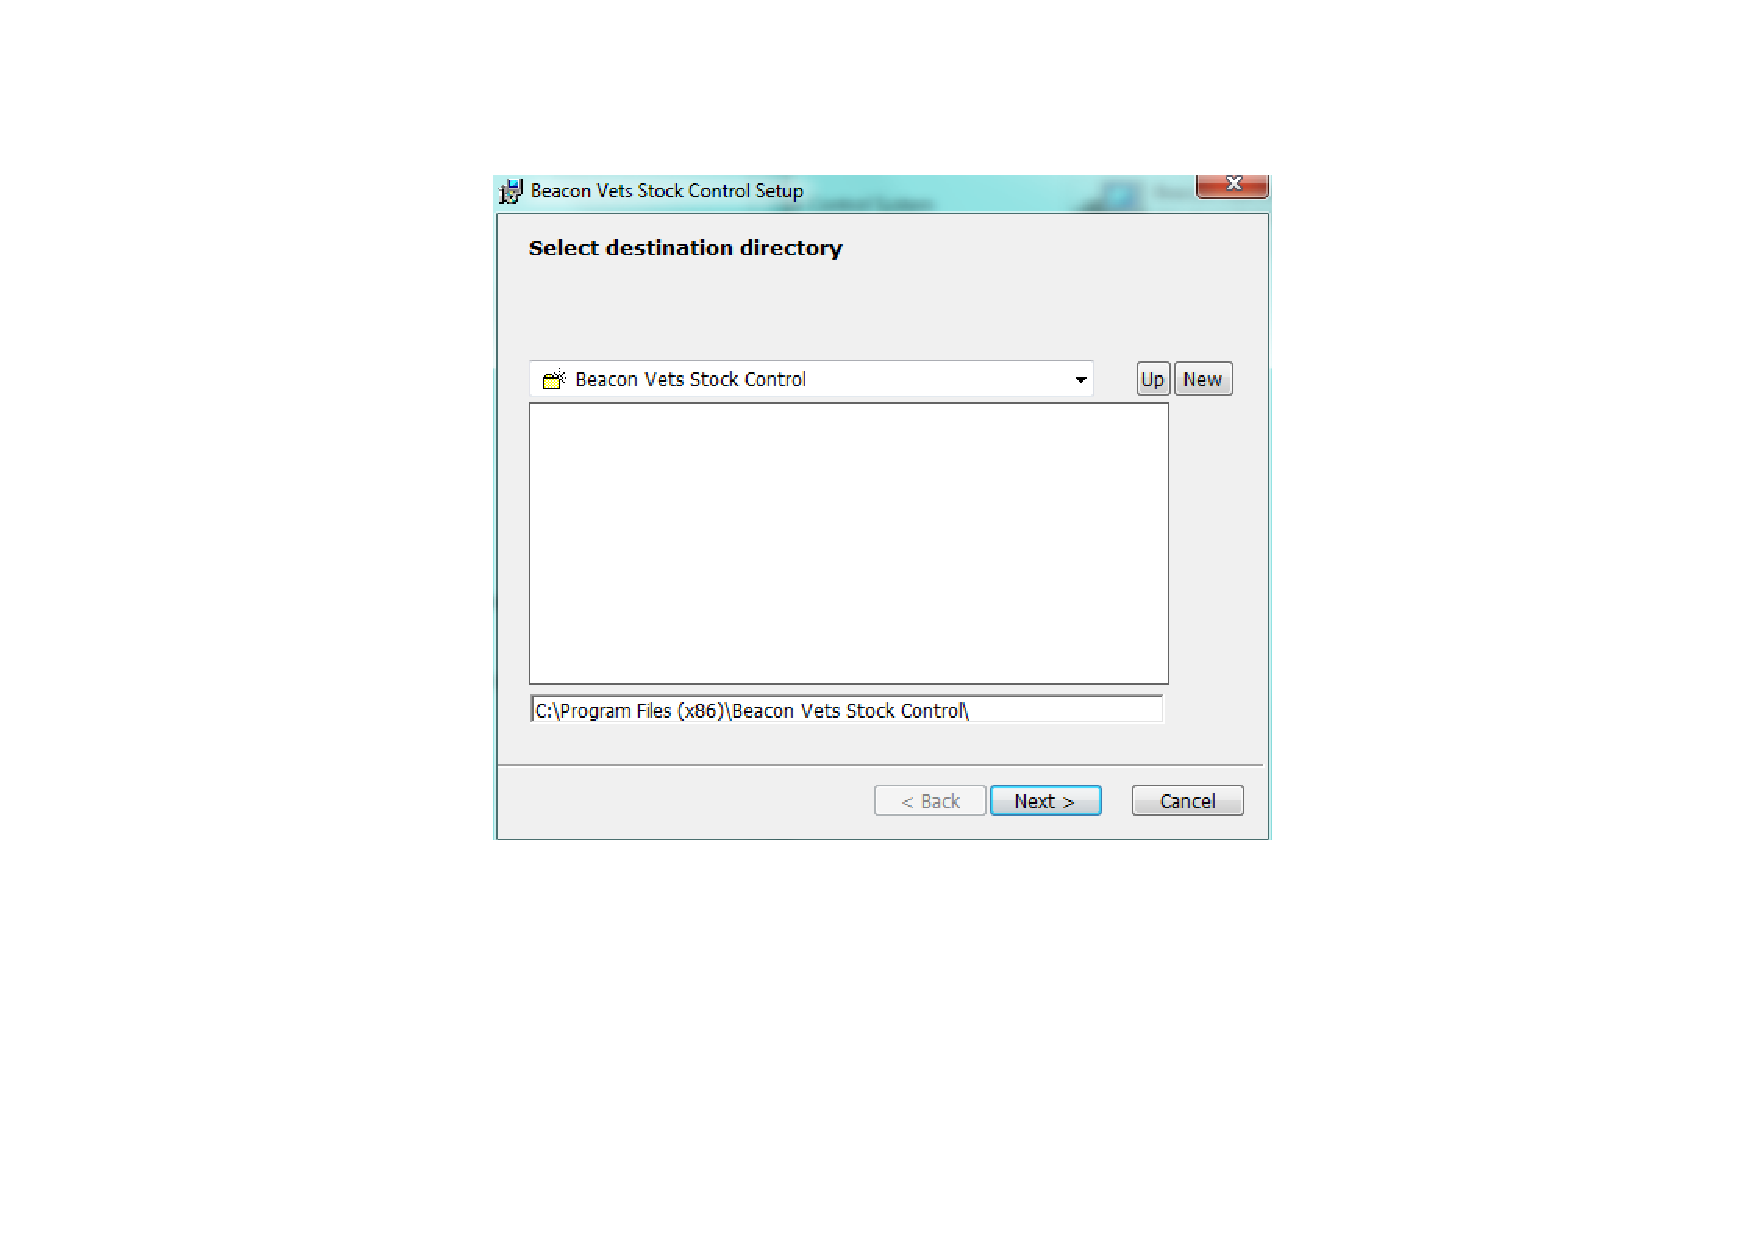
\includegraphics[width=\textwidth]{./ManualImages/install-5.pdf}

\pagebreak

\textbf{6.} Here, you choose where to install the system, find and select the folder `Stock Control System' in which you have just created.

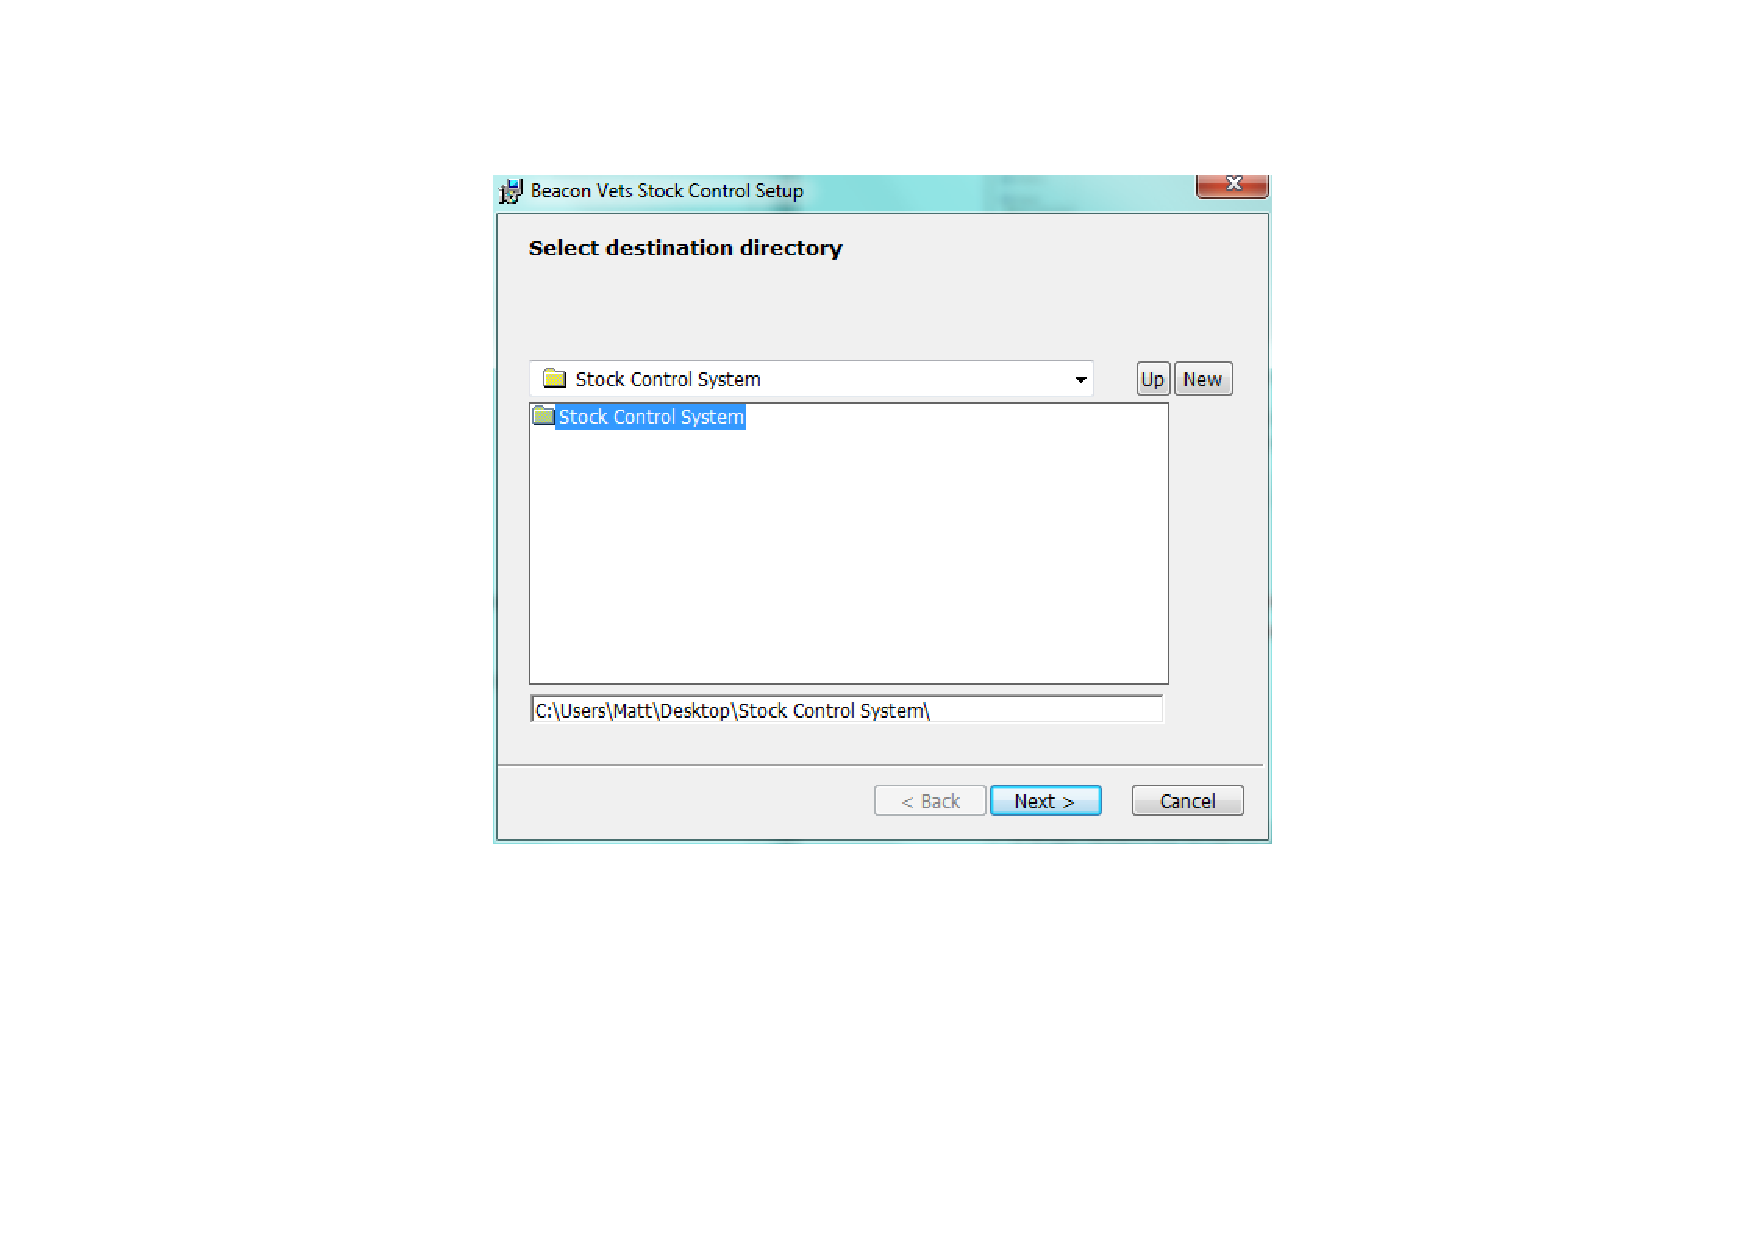
\includegraphics[width=\textwidth]{./ManualImages/install-6.pdf}

\pagebreak

\textbf{7.} Click the `Next' button.

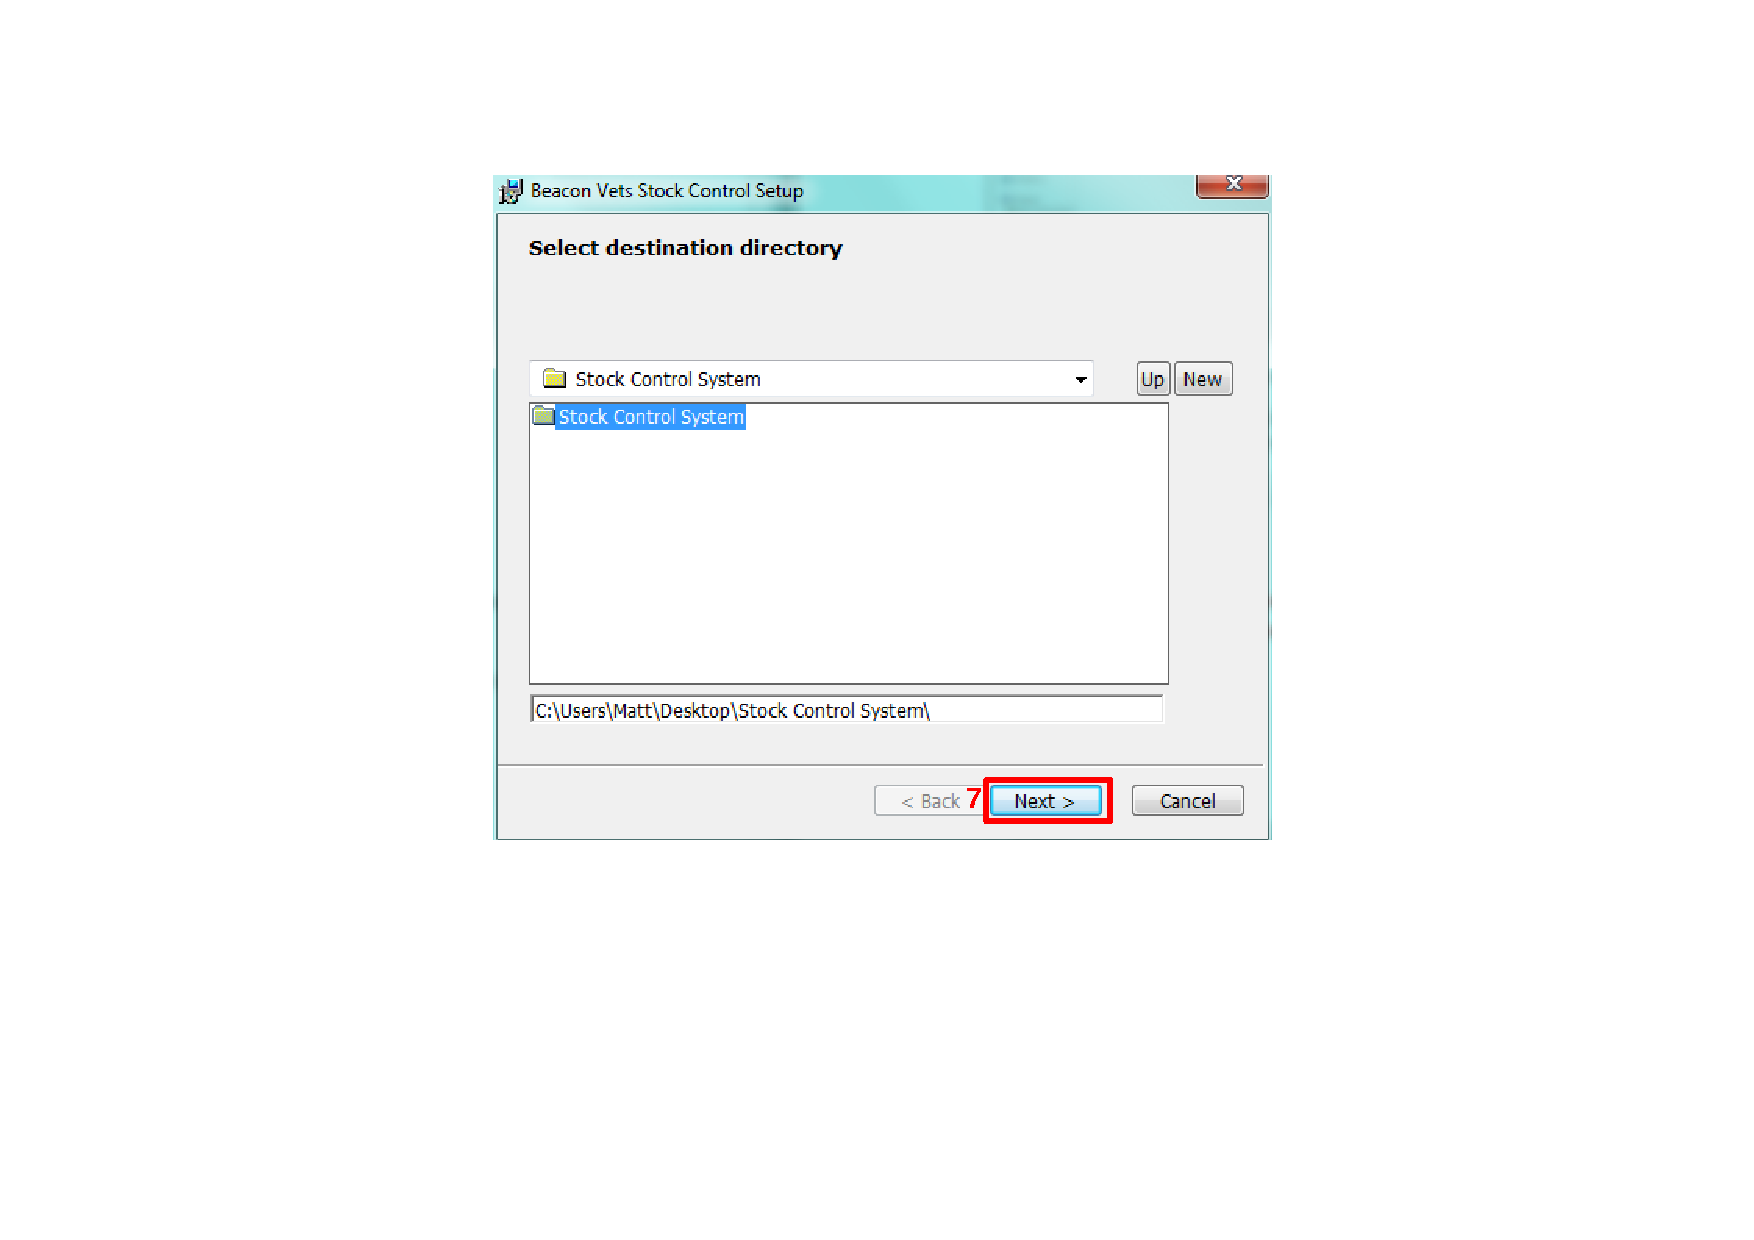
\includegraphics[width=\textwidth]{./ManualImages/install-7.pdf}

\pagebreak

You shall be presented with this screen:

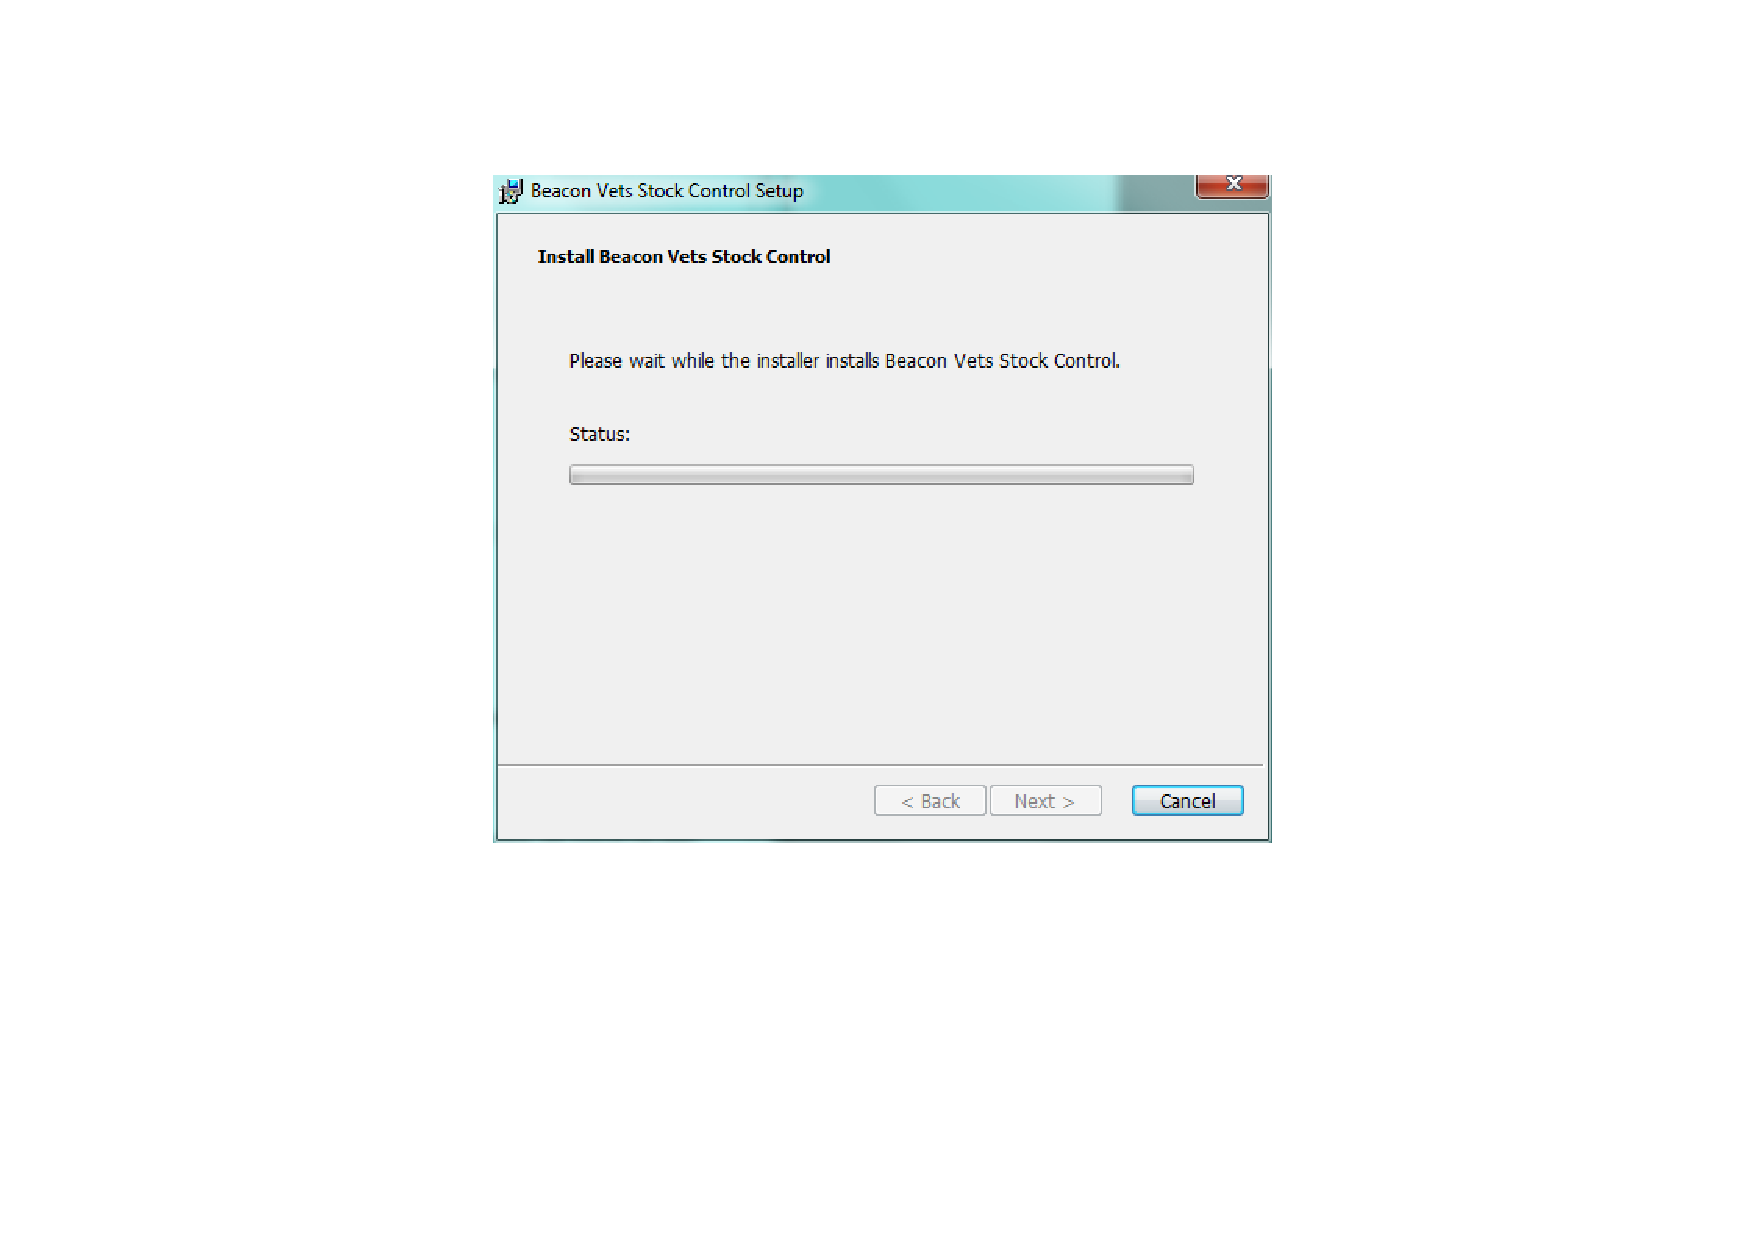
\includegraphics[width=\textwidth]{./ManualImages/install-8.pdf}

\pagebreak

\textbf{8.} After a few seconds, the icon below will display in the taskbar. Click on it.

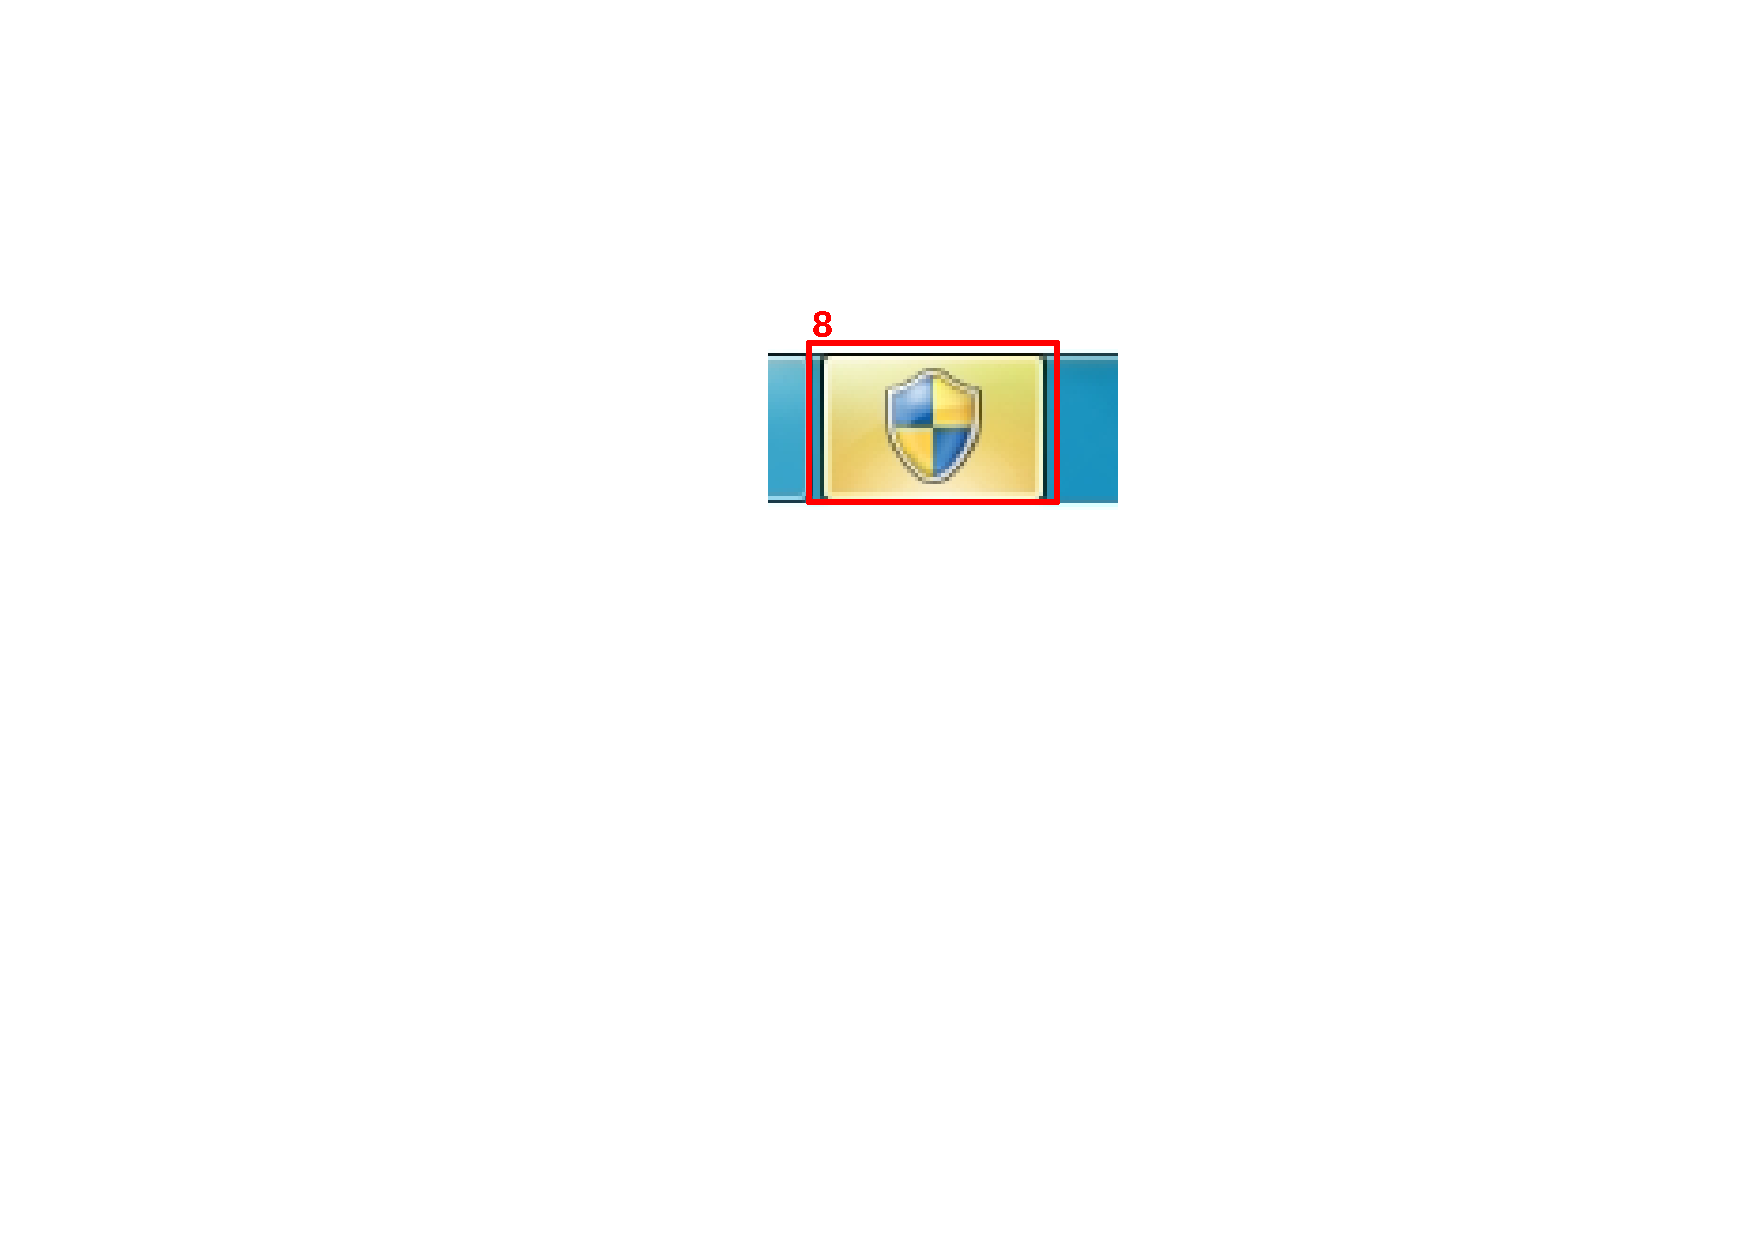
\includegraphics[width=\textwidth]{./ManualImages/install-9.pdf}

\pagebreak

\textbf{9.} The Window below will be displayed, click on the `Yes' button.

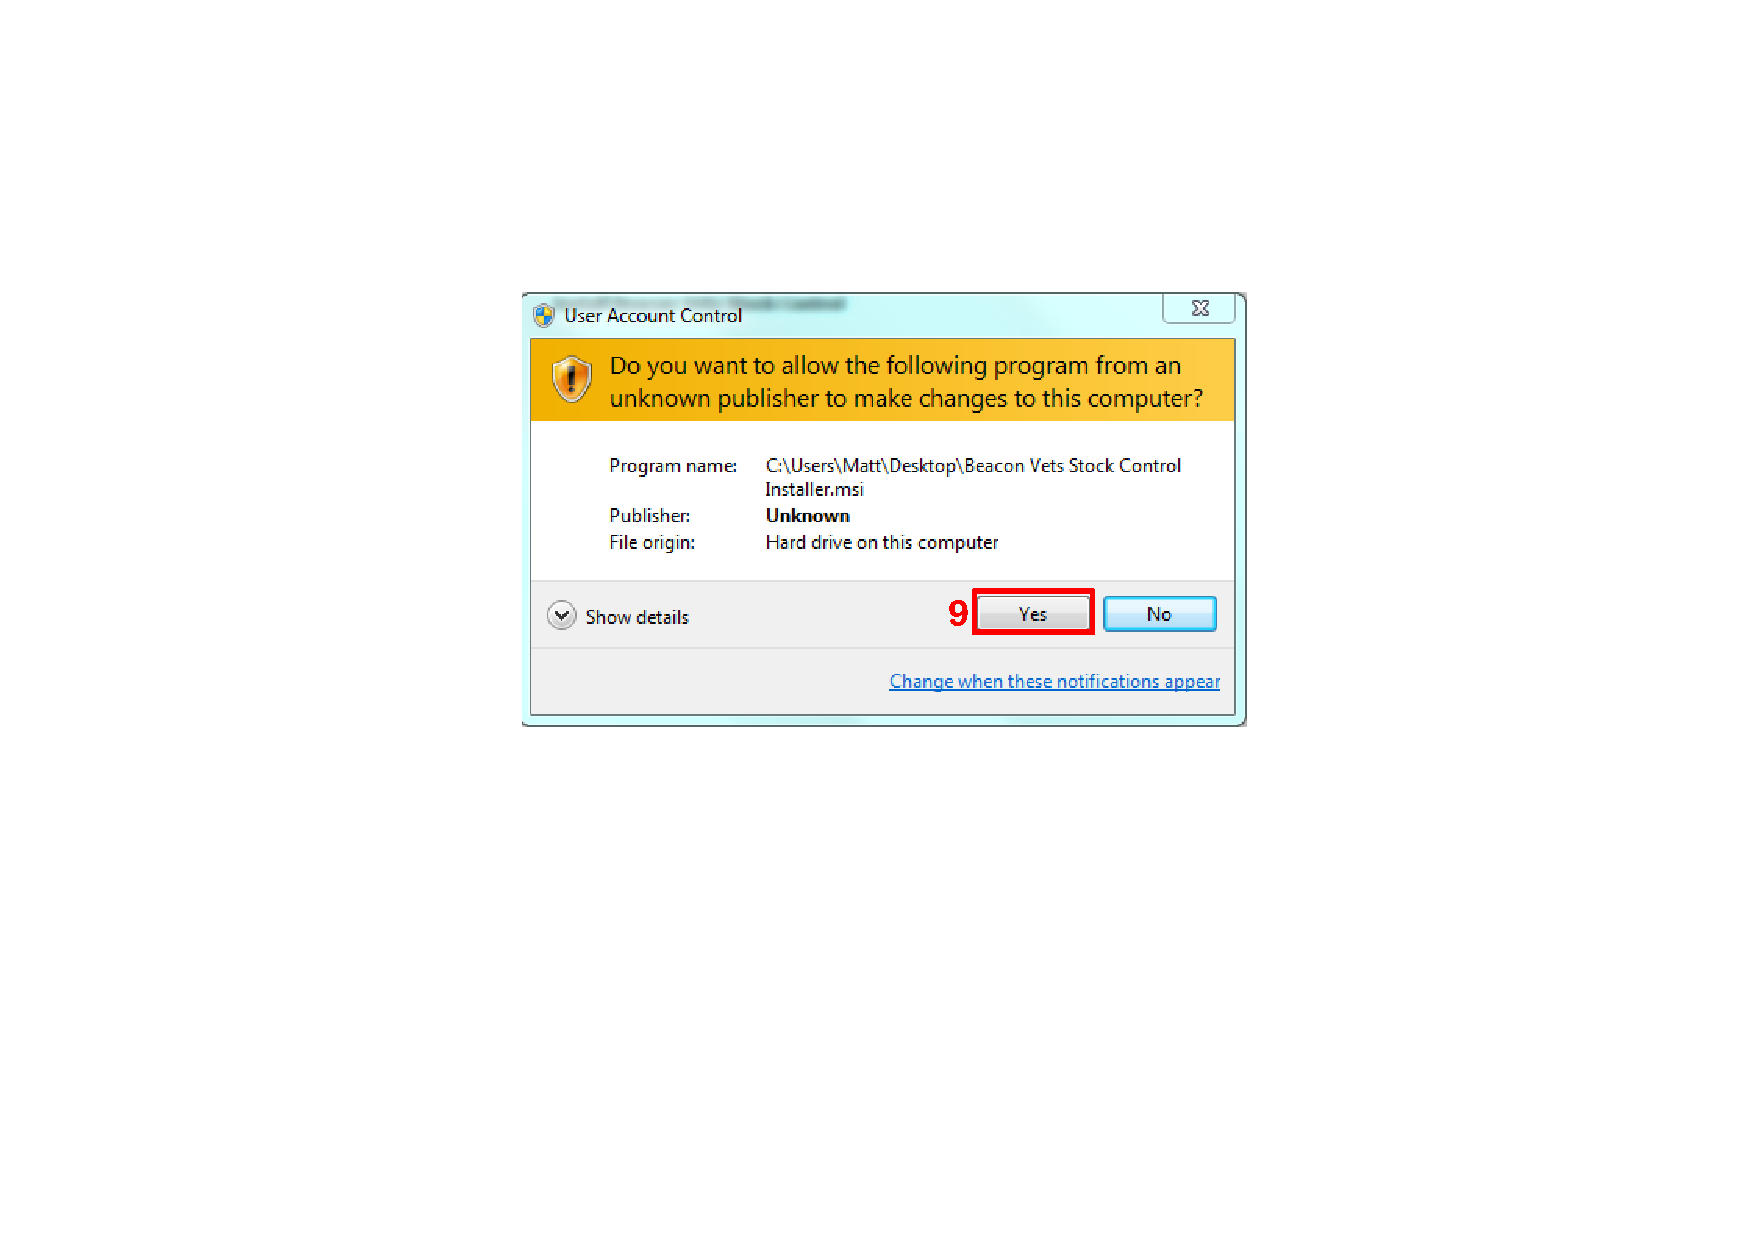
\includegraphics[width=\textwidth]{./ManualImages/install-10.pdf}

\pagebreak

\textbf{10.} Once the program has finished installing, click the `Finish' button.

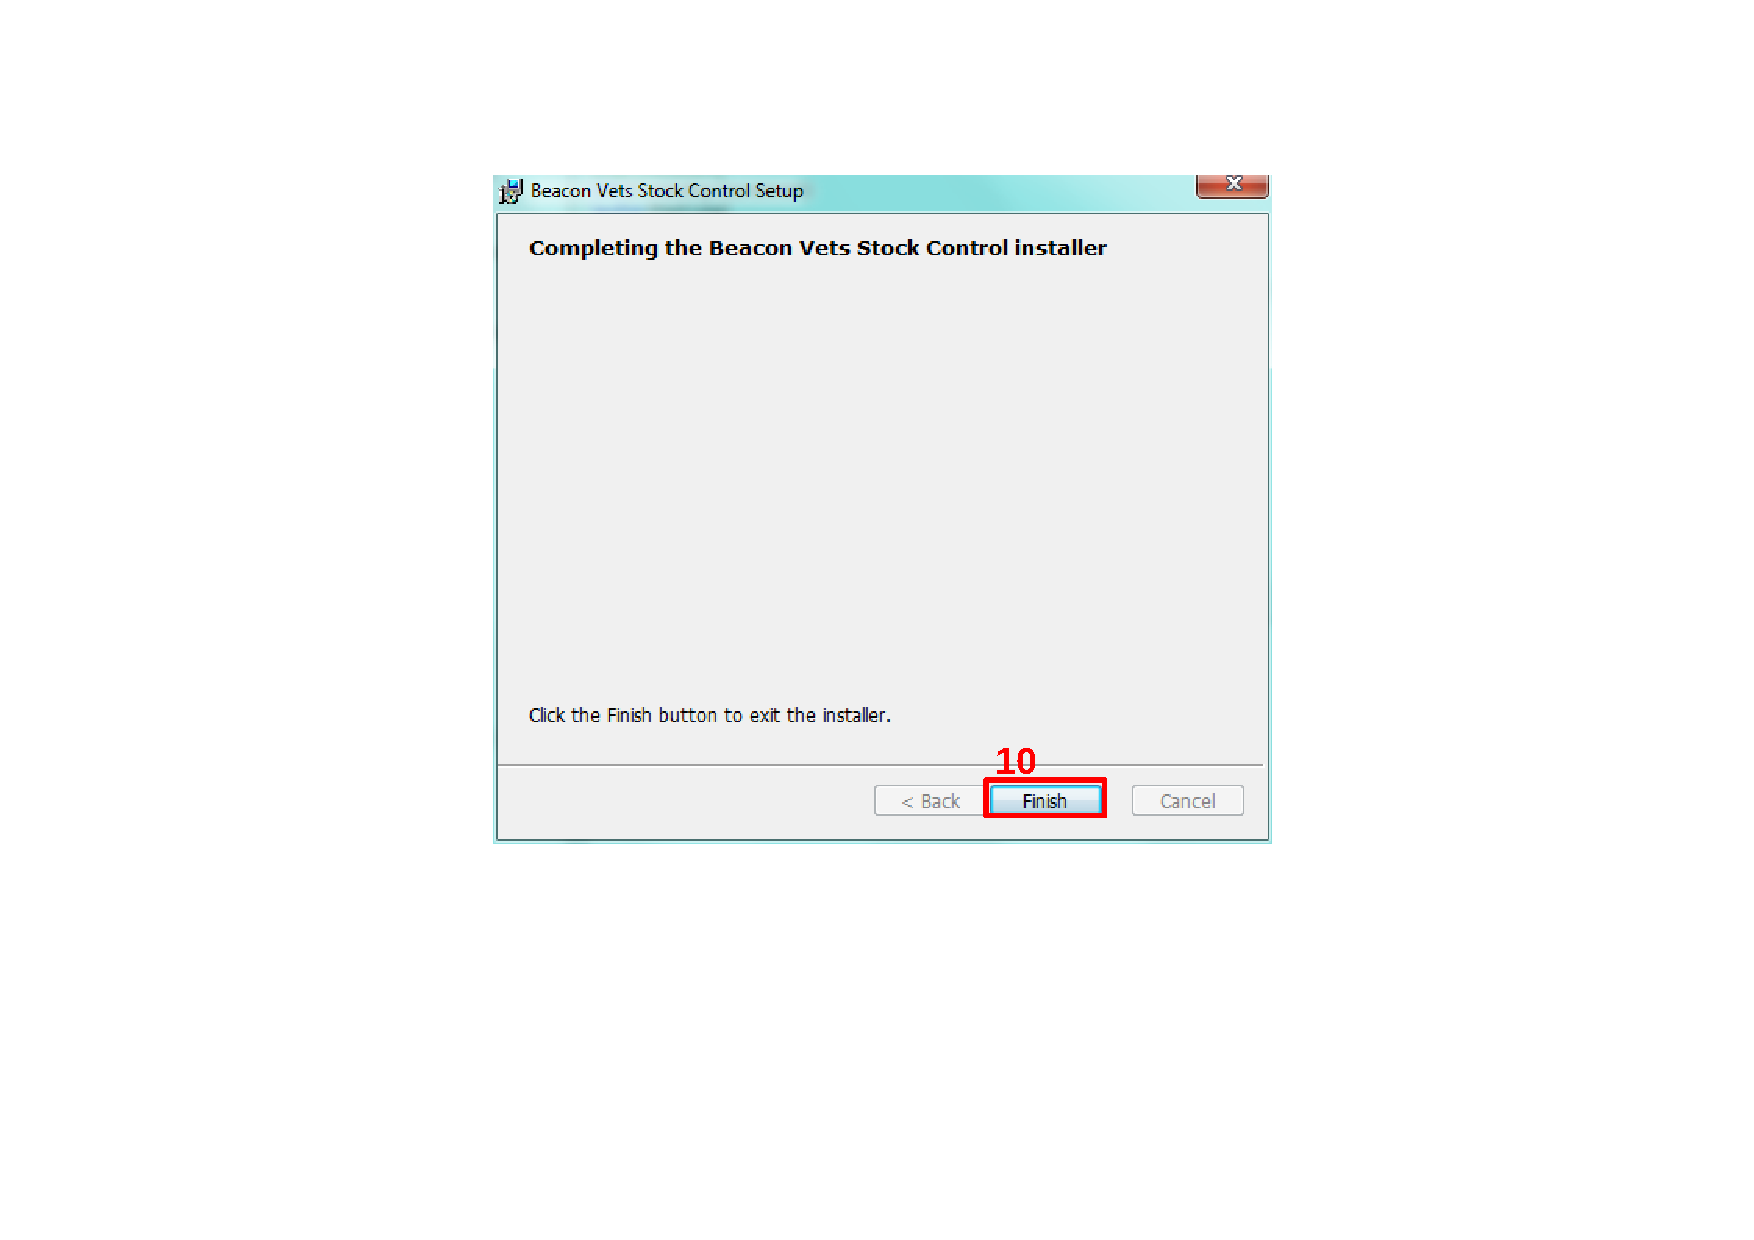
\includegraphics[width=\textwidth]{./ManualImages/install-11.pdf}

You have now successfully installed the system onto your computer. For a tutorial on running the system, go to page \pageref{fig:Running the System}

\pagebreak

\subsection{Running the System}
\label{fig:Running the System}

\textbf{1.} Locate the `Stock Control System' folder created during the system installation. If you have not already done the system installation, this can be found on page \pageref{fig:System Installation}.

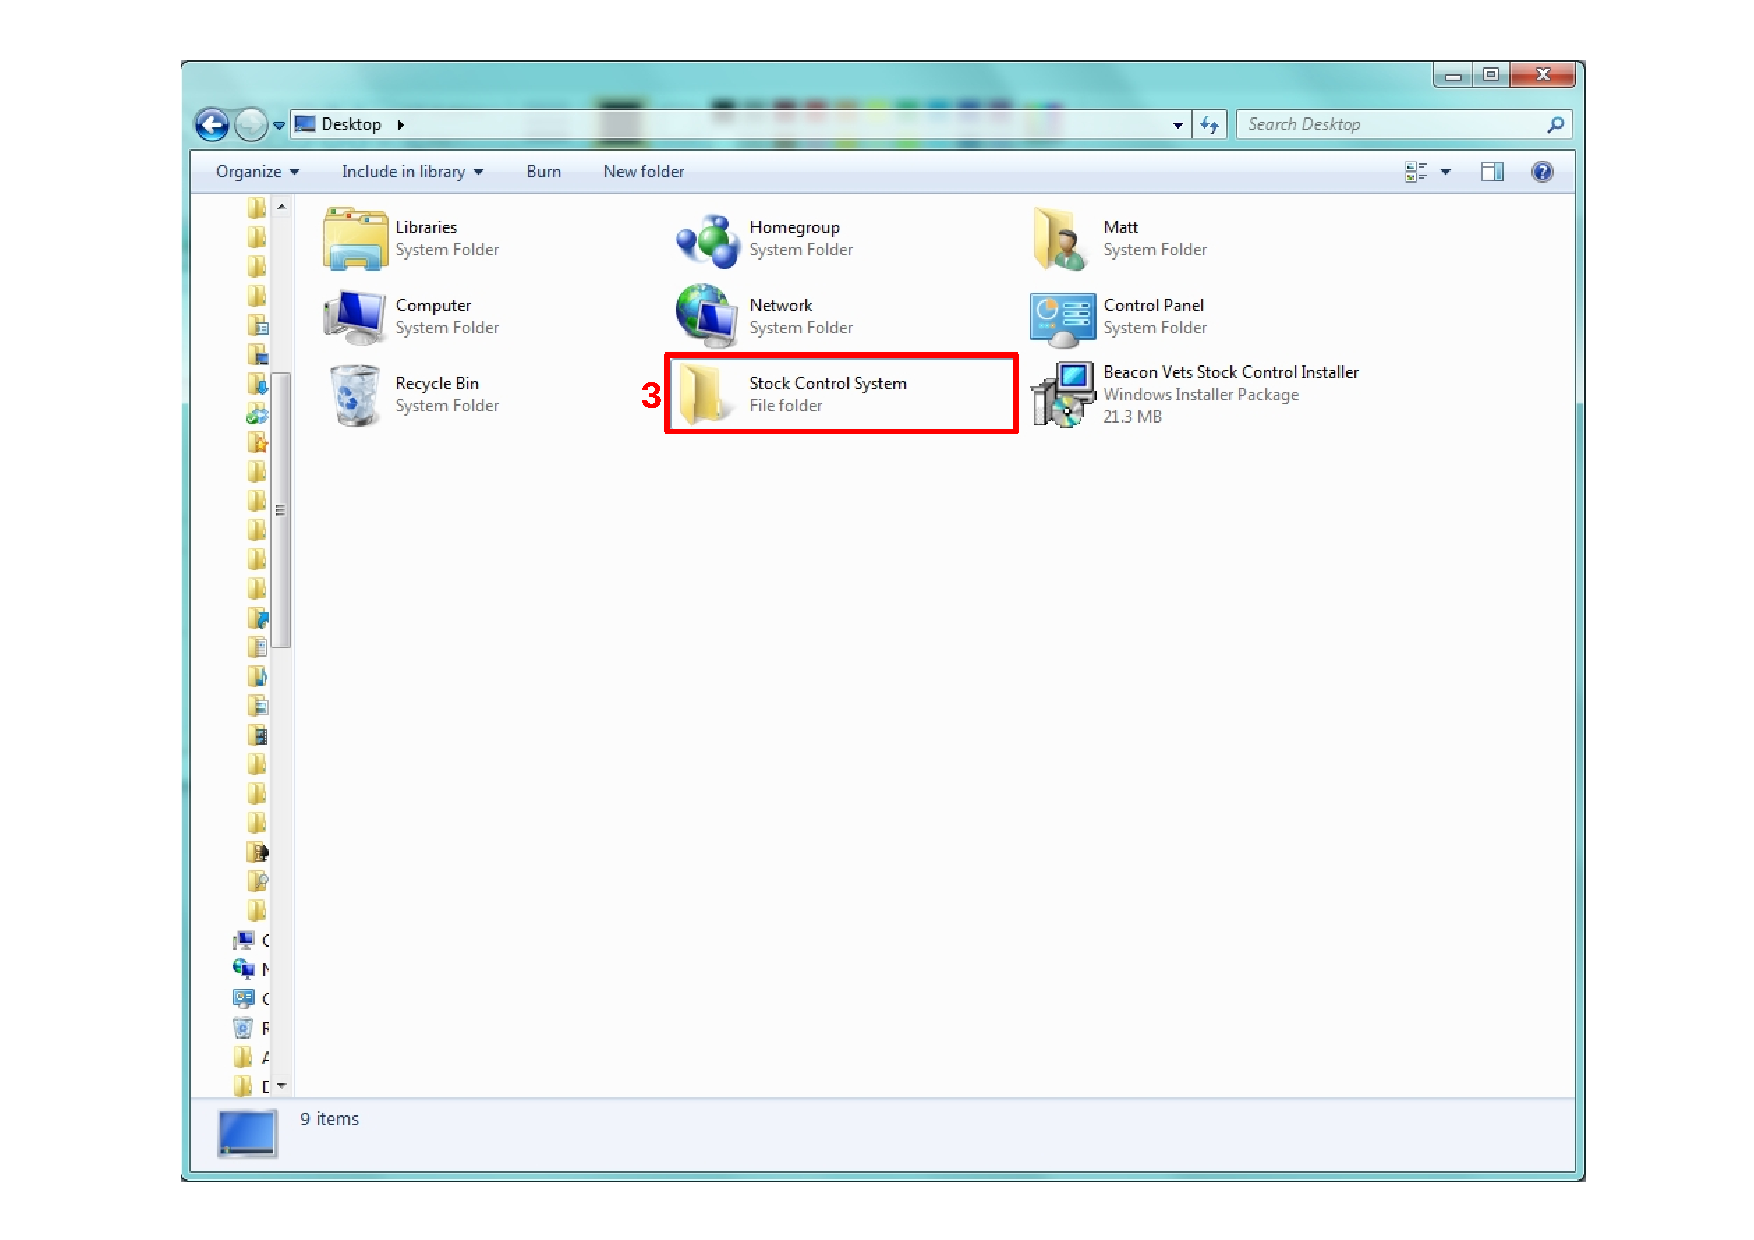
\includegraphics[width=\textwidth]{./ManualImages/install-3.pdf}

\textbf{2.} Double left click on the folder to open it. There should be many different files within this folder.

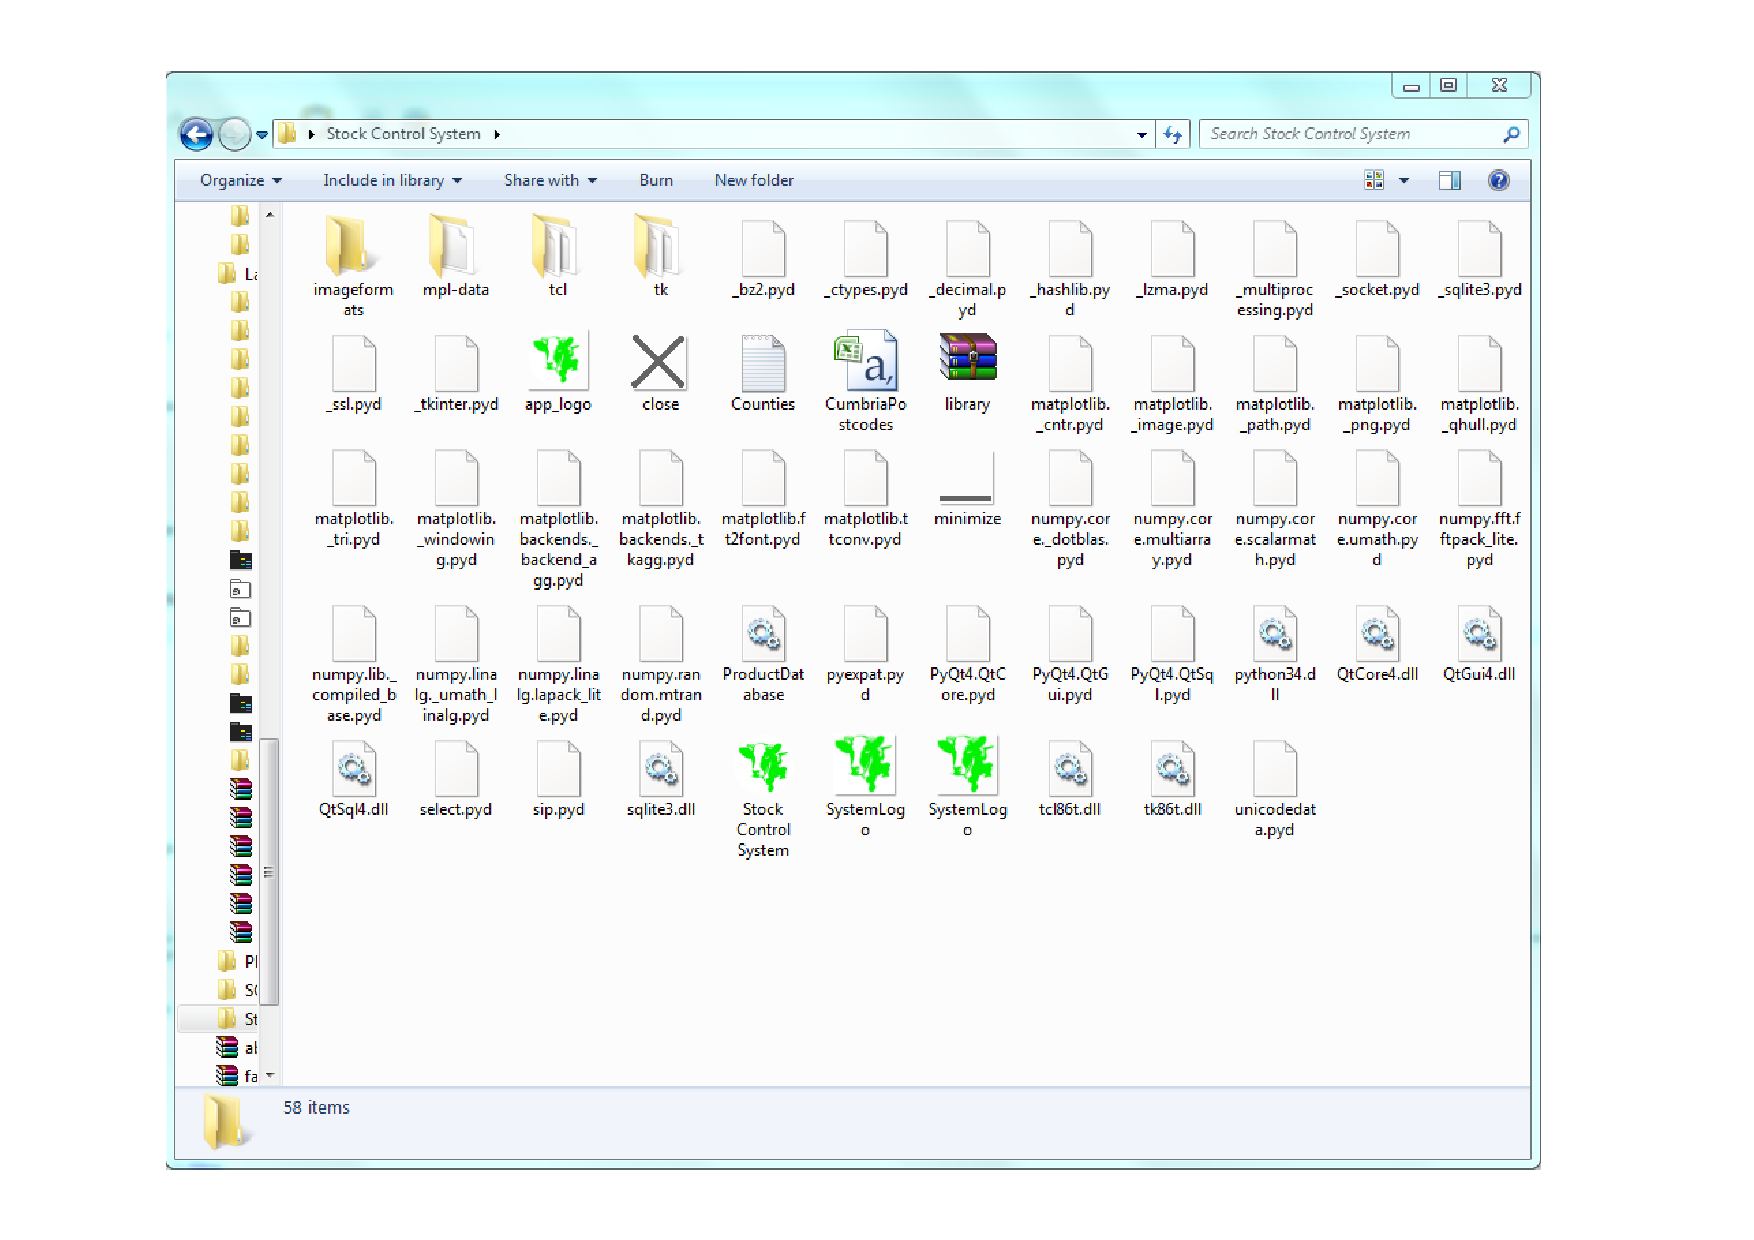
\includegraphics[width=\textwidth]{./ManualImages/install-12.pdf}

\textbf{3.} You need to locate the file named `Stock Control System'.

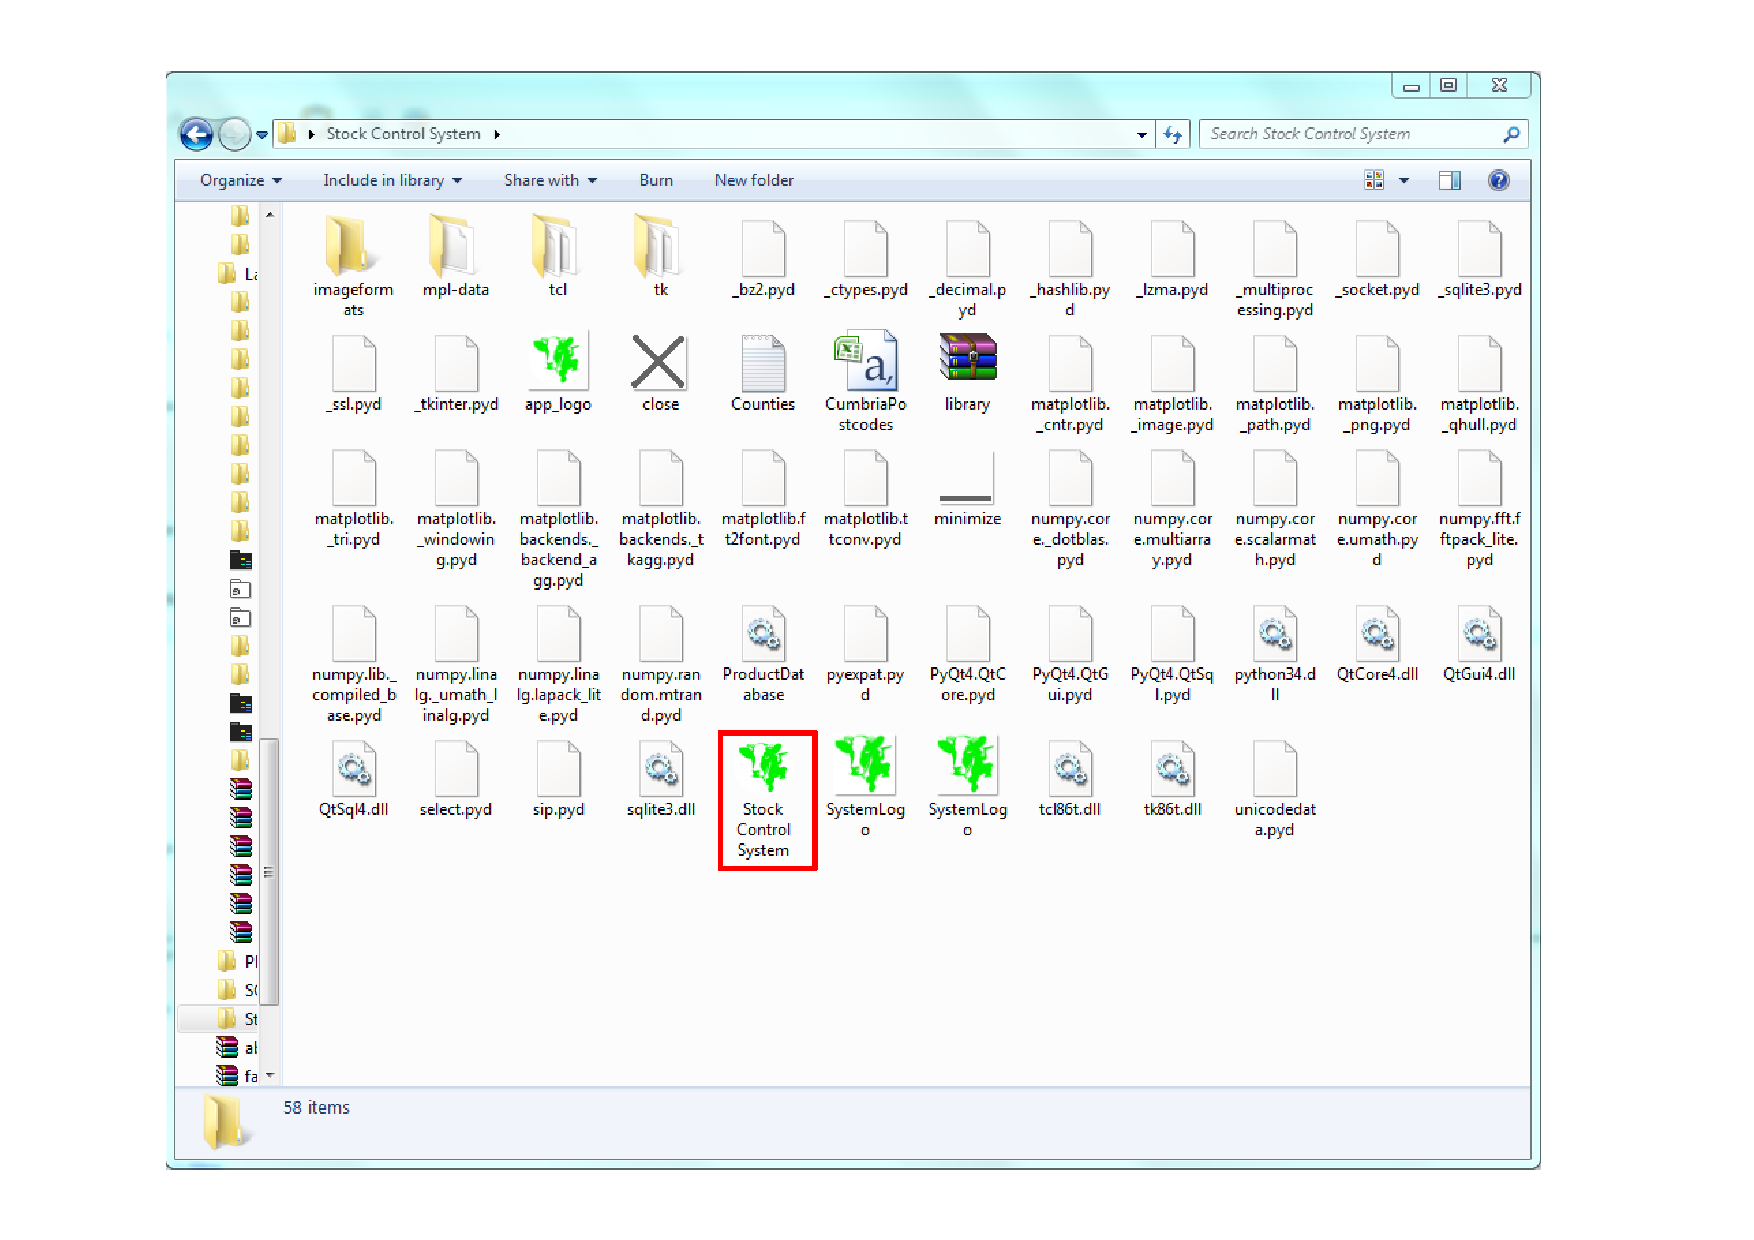
\includegraphics[width=\textwidth]{./ManualImages/install-13.pdf}

\textbf{4.} Double left click on this file and wait a couple of seconds. The first start up of the system takes a while to create the database file. The Log in screen will then display.

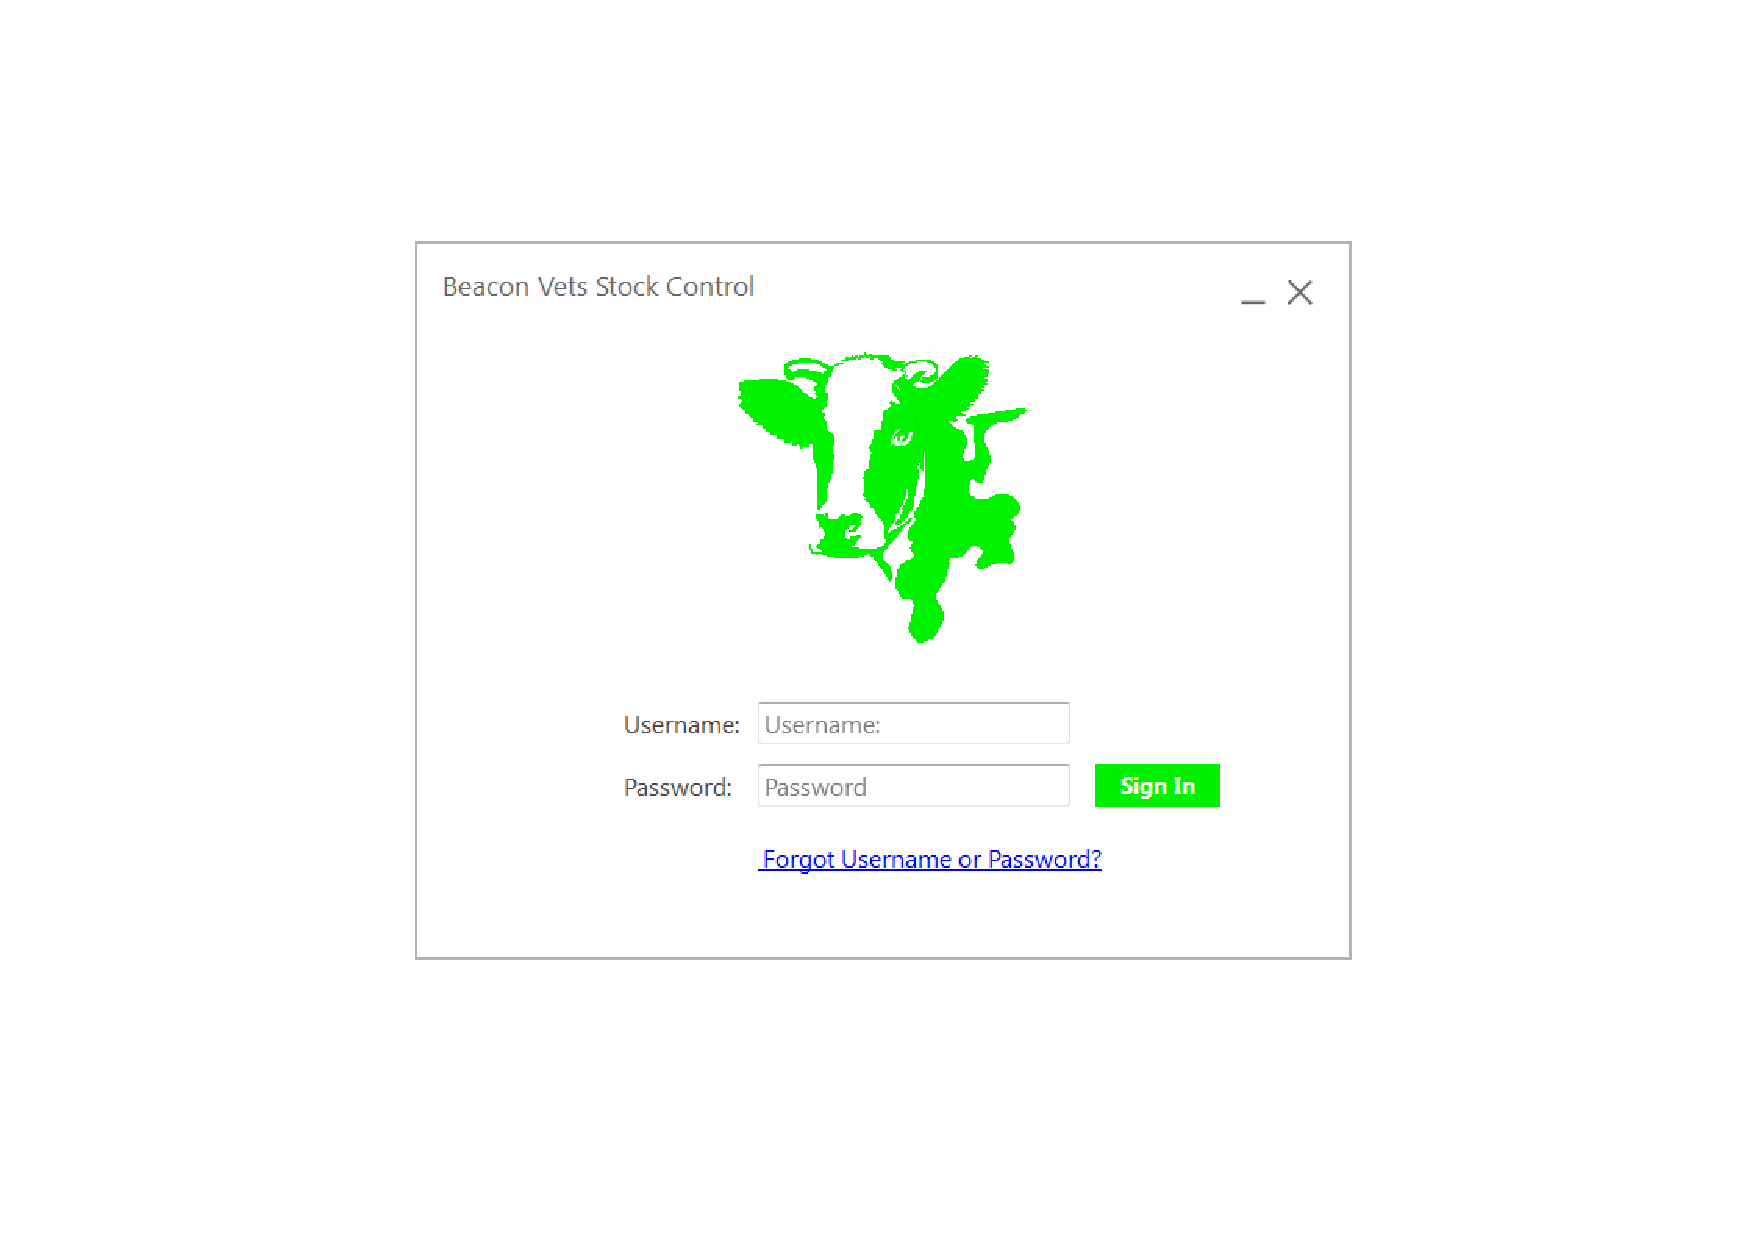
\includegraphics[width=\textwidth]{./ManualImages/install-14.pdf}

The system is now successfully running! To close the system, click on the `X' button in the top right hand corner of the window.

\pagebreak

The Following instructions show you know to make the system more easily accessible. This is not required for the system to run, but helps you to get the system running a lot faster.

\subsubsection{Creating a Desktop Icon}

\textbf{1.} Repeat steps 1 to 3 from the `Running The System' section. Once you have located the `Stock Control System' file, right click on it and select the `Create Shortcut' option from the drop down menu.

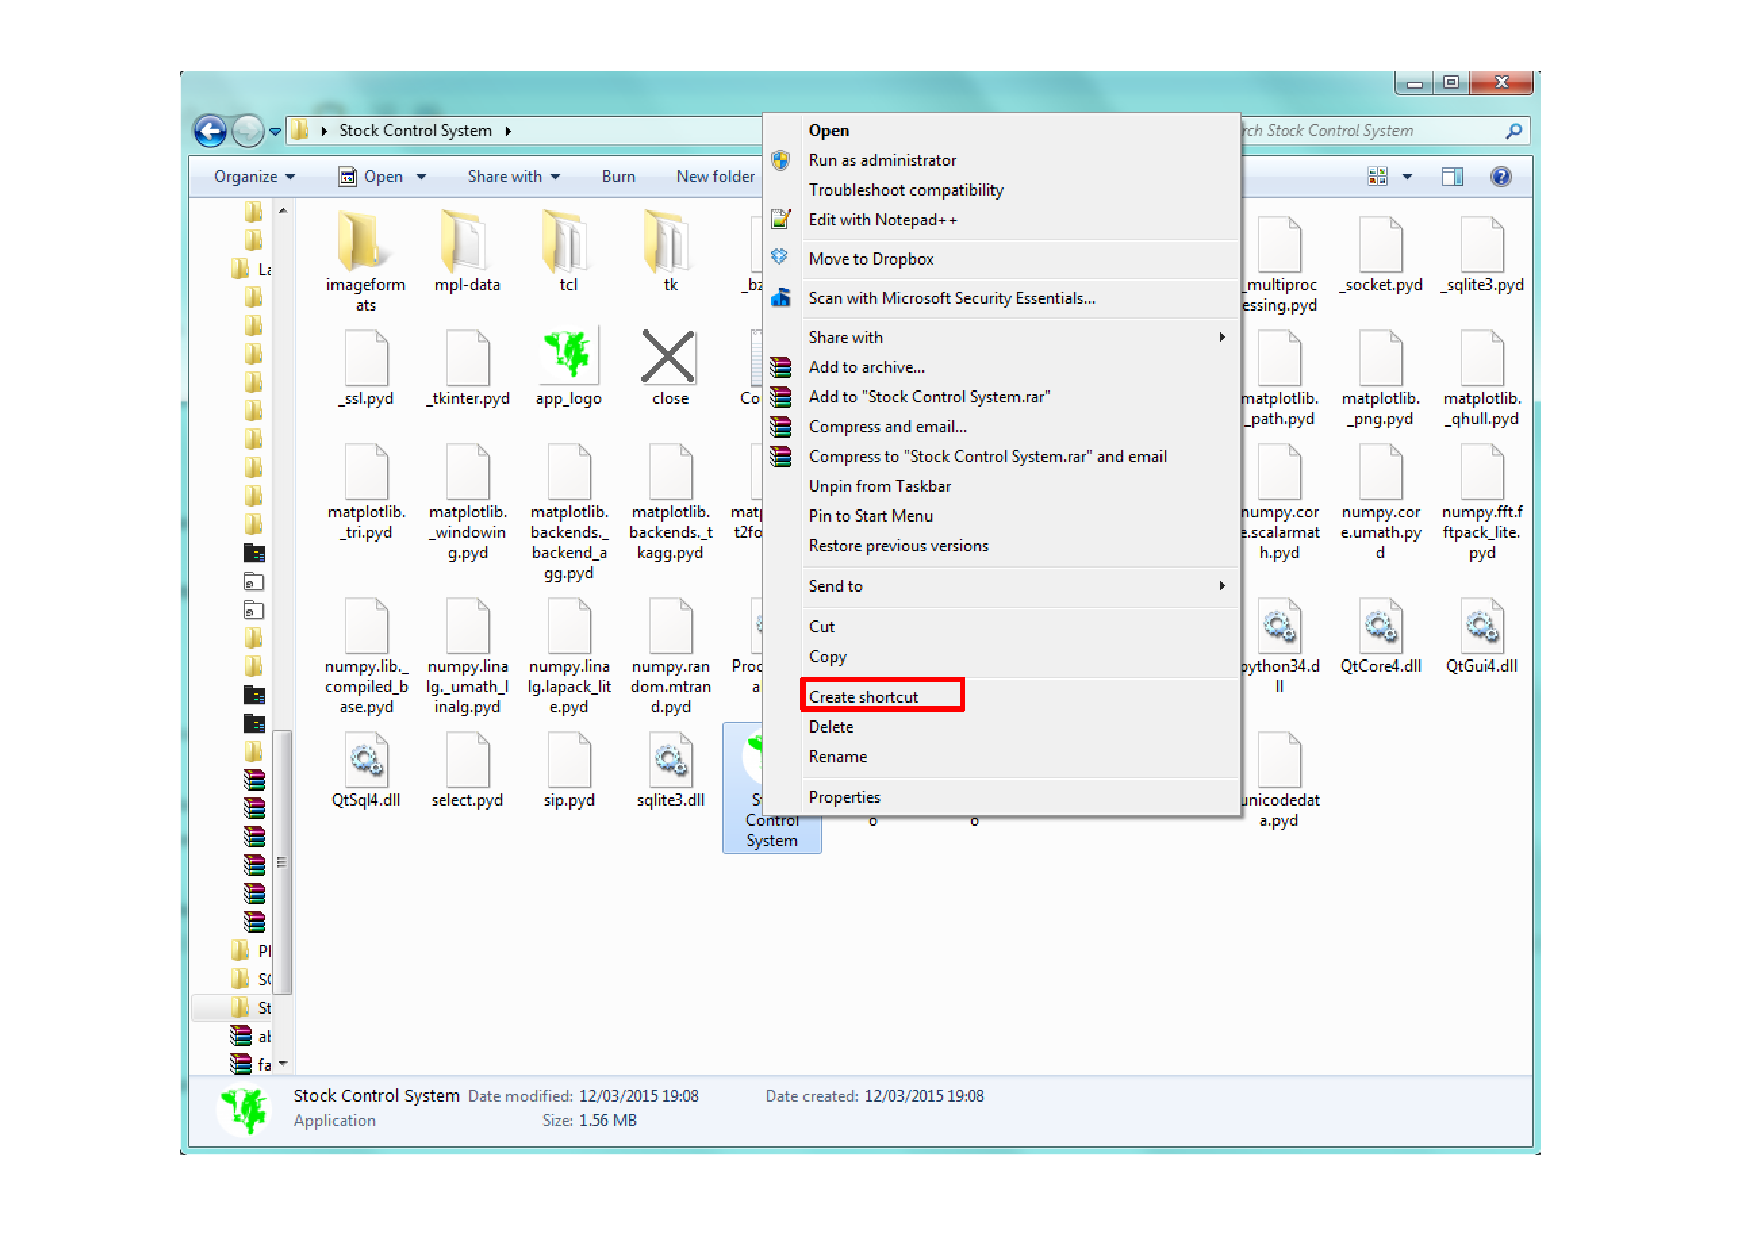
\includegraphics[width=\textwidth]{./ManualImages/install-15.pdf}

\textbf{2.} A file called `Stock Control System - Shortcut' will be created once the `Create Shortcut' button is clicked. Drag and drop this file onto the desktop.

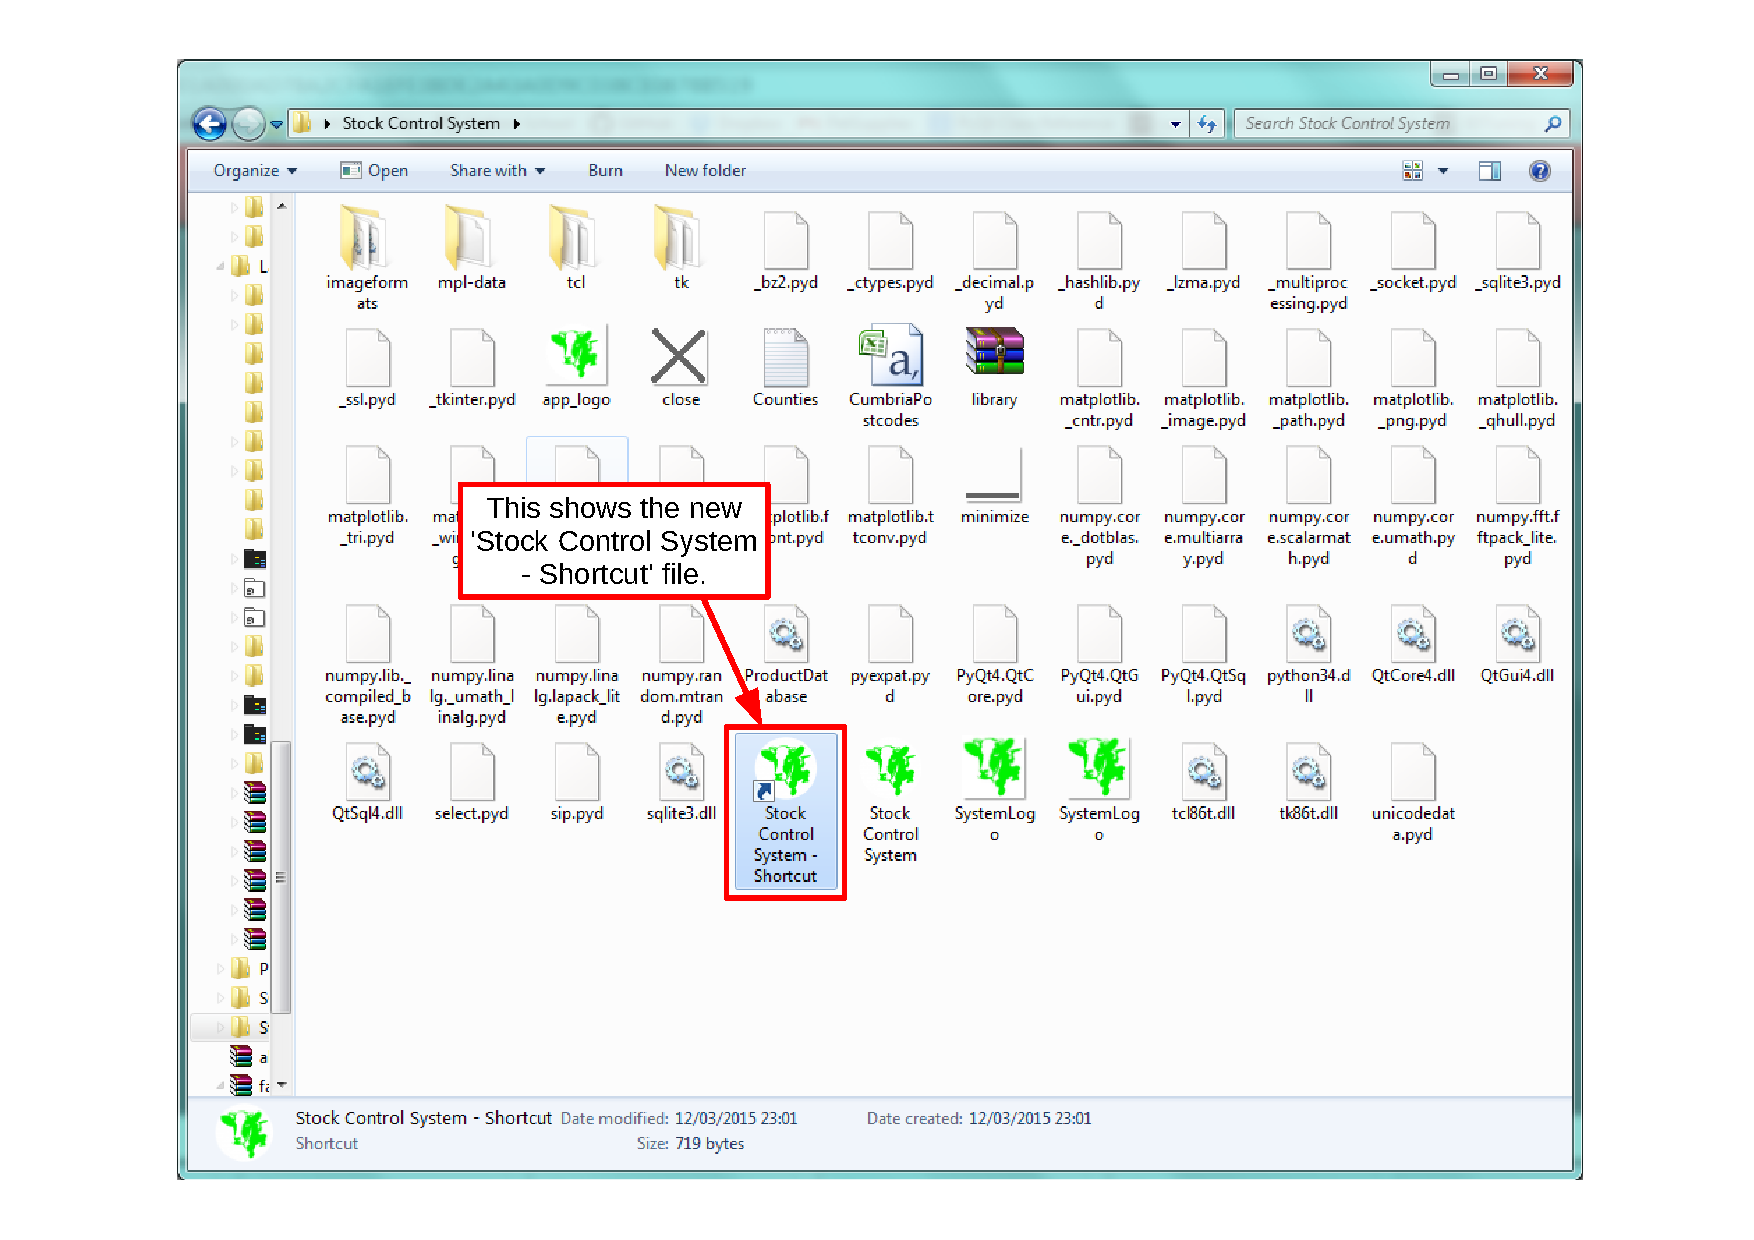
\includegraphics[width=\textwidth]{./ManualImages/install-16.pdf}

Now that the shortcut has been placed on the desktop, the shortcut can be double left clicked to quickly access the system from the desktop.

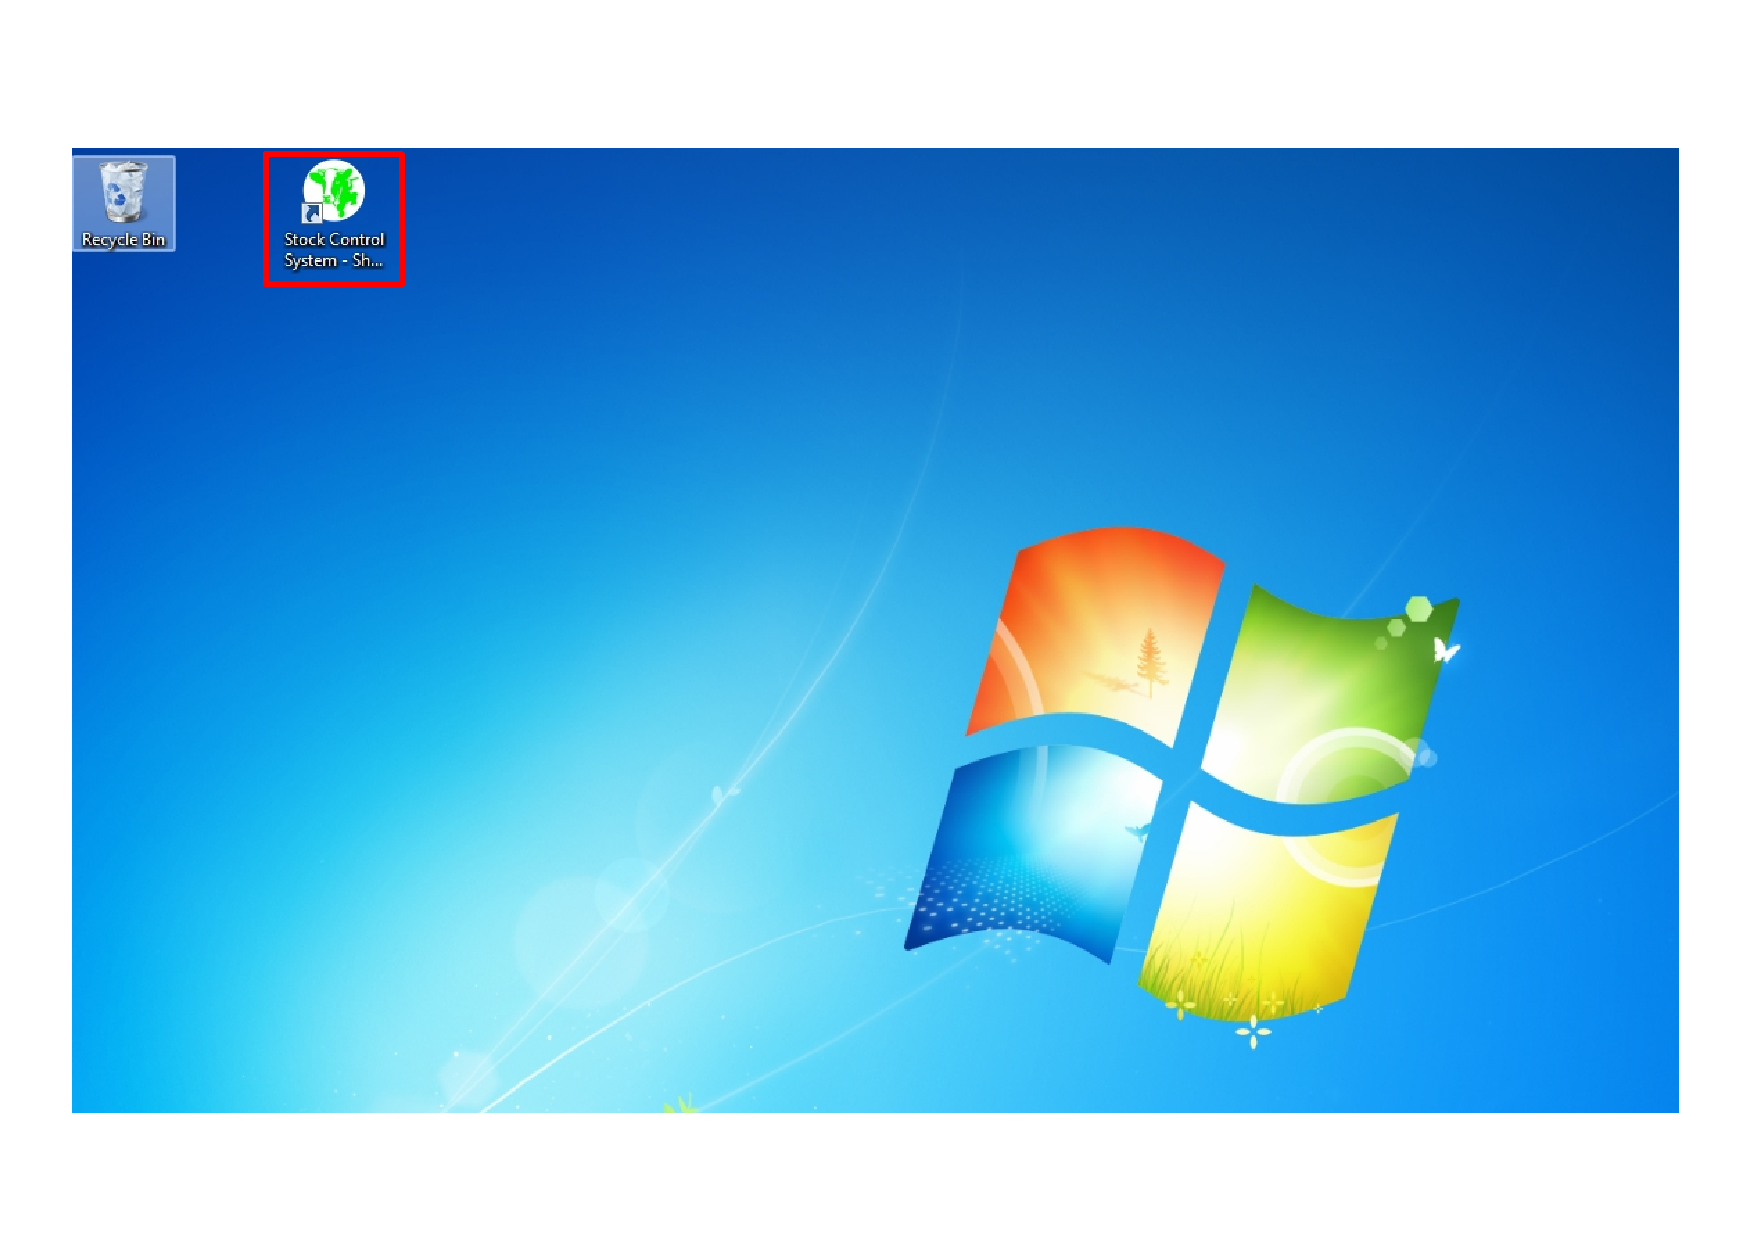
\includegraphics[width=\textwidth]{./ManualImages/install-17.pdf}

\subsubsection{Pinning the system to the taskbar}

Pinning the system to the taskbar will provide you with the fastest way to run the system.

\textbf{1.} Repeat steps 1 to 4 in the `Running the System' section. Whilst you are on the log in screen, the system icon should be displayed in the taskbar.

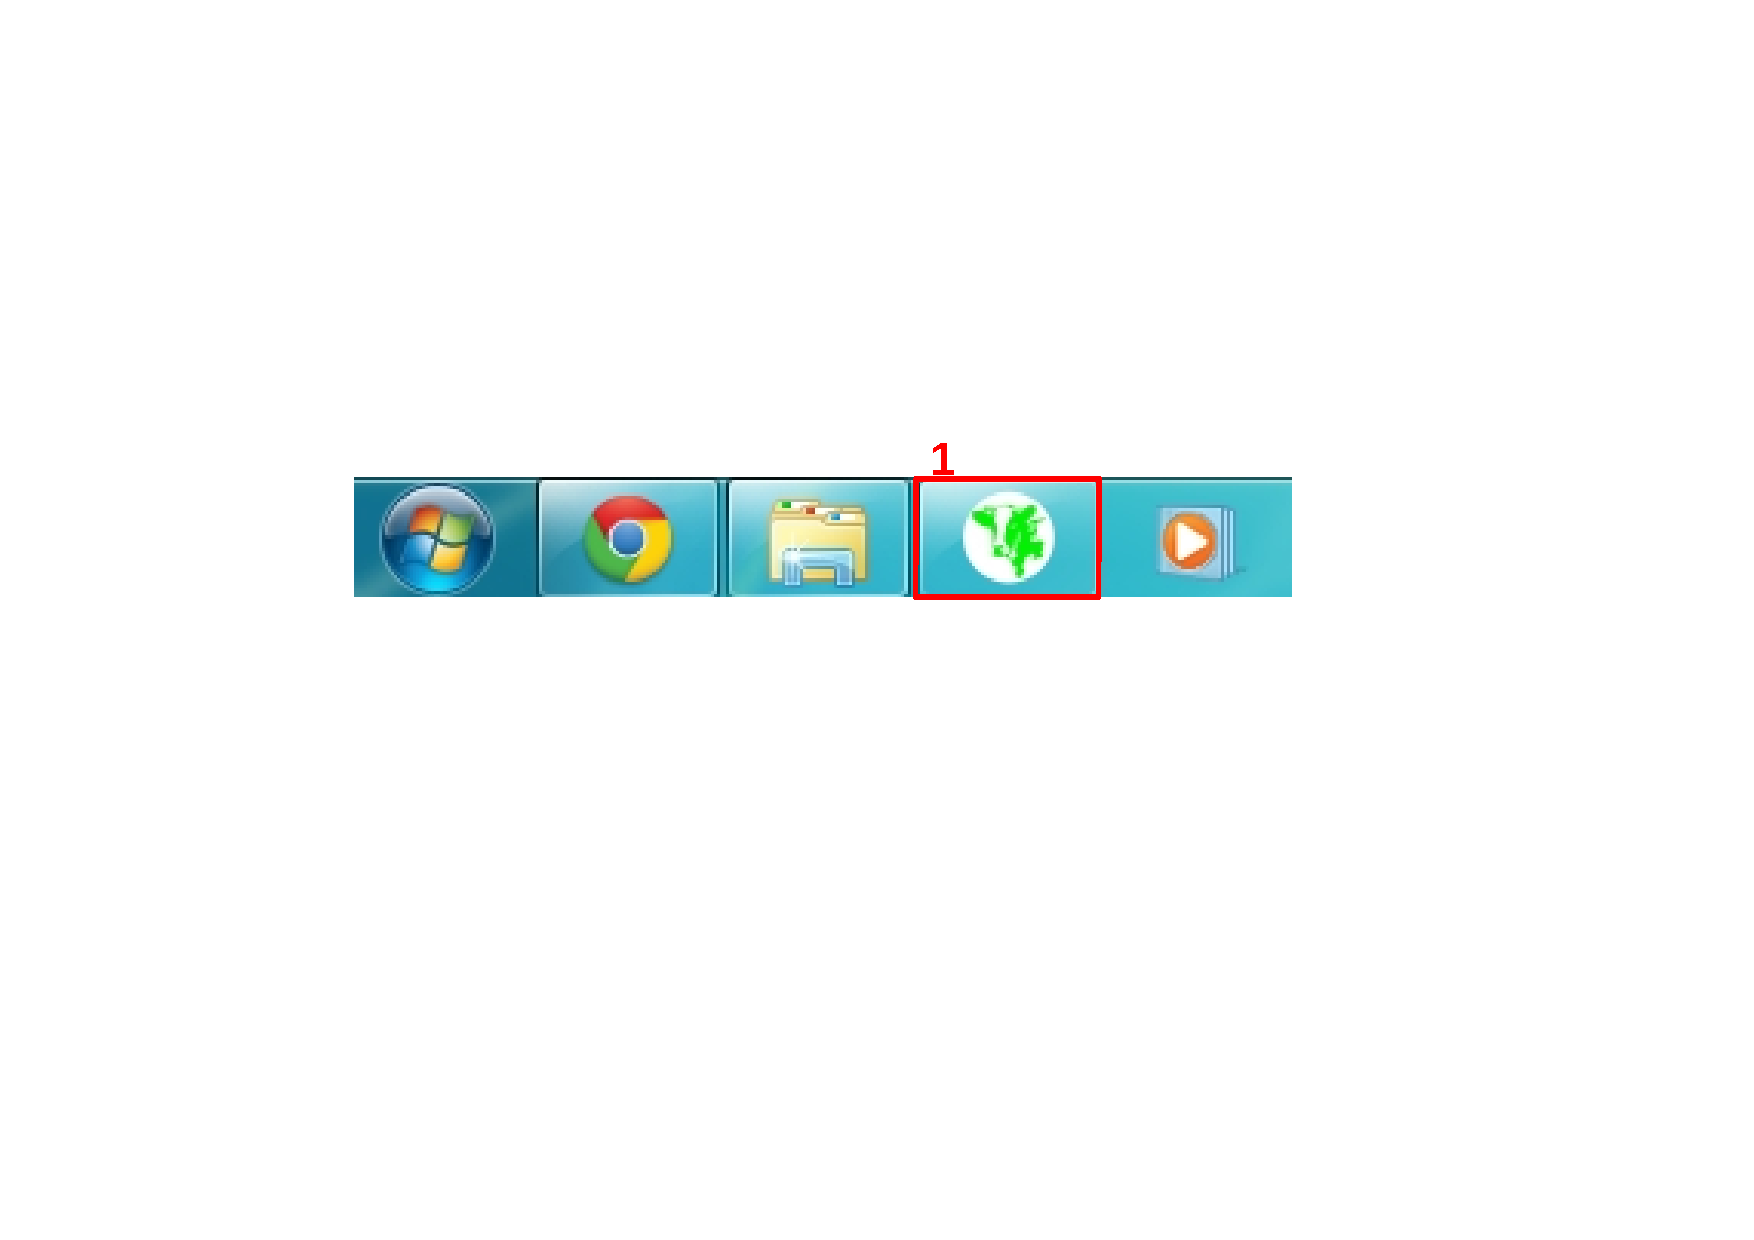
\includegraphics[width=\textwidth]{./ManualImages/install-18.pdf}

\textbf{2.} Right click on the icon in the taskbar and click the `Pin this program to the taskbar' option, in the menu.

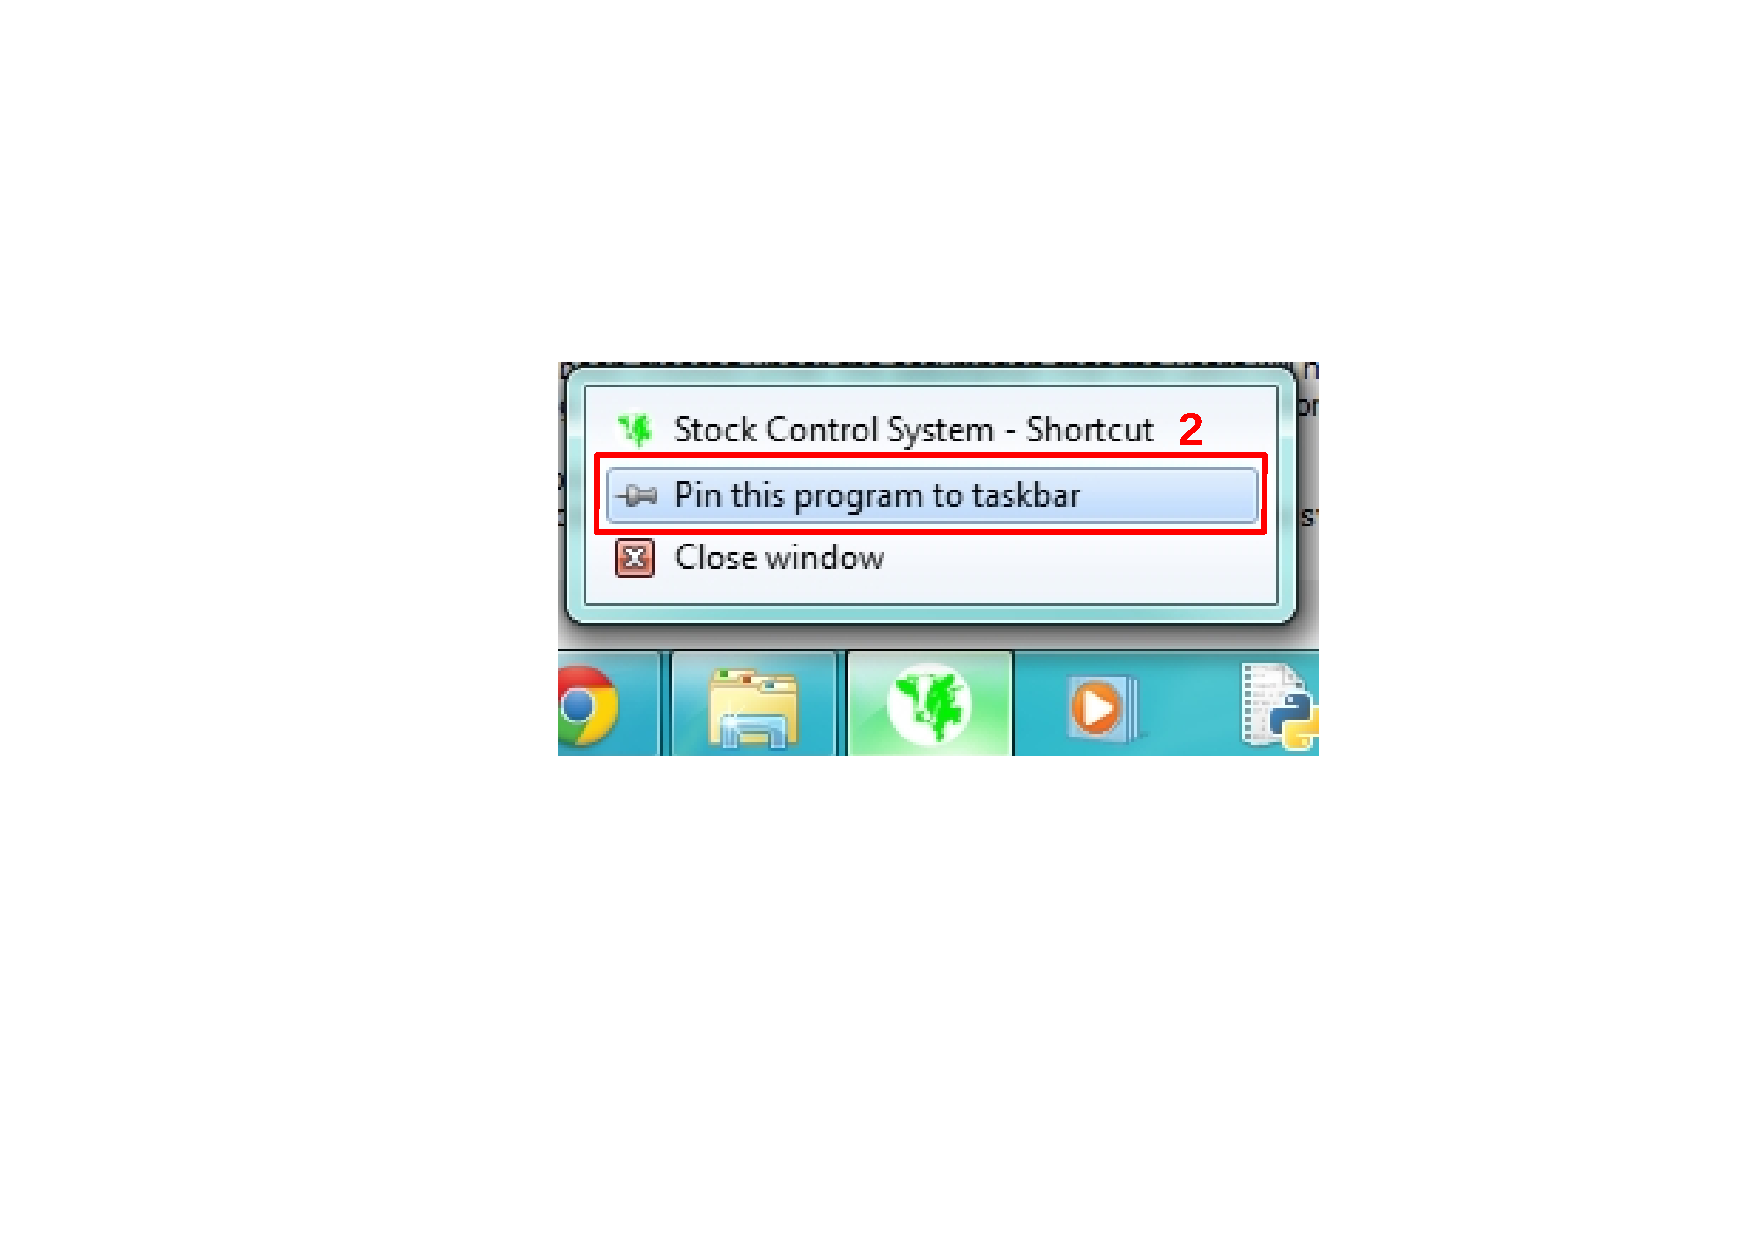
\includegraphics[width=\textwidth]{./ManualImages/install-19.pdf}

Now that the program is pinned to the taskbar, whenever you want to run the system, simply left click the system icon in the taskbar and the system will run.

\pagebreak

\section{Tutorial}

\subsection{Introduction}
The following section explains how to use each component of the system. Each subsection of the tutorial gives a detailed explanation including annotated diagrams to assist you in running the system.


\subsection{Assumptions}

The Tutorial has been created under the assumption that the users will have a variety of different computer knowledge. Therefore, the tutorial has been created such that, minimal computer knowledge is required to understand it. Another assumption made, is that the system has been installed successfully, and that the system is already running. The installation tutorial can be found on page \pageref{fig:System Installation} and the tutorial on running the system can be found on page \pageref{fig:Running the System}

\subsection{Tutorial Questions}
The following sections are a step by step guide for each section of the system. The different sections of the tutorial have been broken down into Questions which can be referenced in the contents table below:

\pagebreak
\subsubsection{Contents}

\begin{center}
    \begin{longtable}{|p{8cm}|p{3cm}|}
        \hline
	 \textbf{Question} & \textbf{Page Number} \\ \hline
	How do I log in to the system? & \pageref{fig:Logging into the system} \\ \hline
	How do I log out of the system? & \pageref{fig:Logging out of the system} \\ \hline
	What should i do if i forget my user-name or password?&  \pageref{fig:Forgetting Your User-name or Password} \\ \hline
	What should i do if i can no longer access the email address associated with my account? &  \pageref{fig:Unable to access your email address} \\ \hline
	How do i add a product to the system? &  \pageref{fig:Adding a Product to the system} \\ \hline
	How do i edit a product that is currently in the system?&  \pageref{fig:Editing a Product in the system} \\ \hline
	How do i remove a product from the system?&  \pageref{fig:Removing a Product from the system} \\ \hline
	How do i change the stock of a product?&  \pageref{fig:Changing the stock of a Product} \\ \hline
	How do i view the predicted sales of a product?&  \pageref{fig:Product Stock Prediction} \\ \hline
	How do i add a Member to the system?&  \pageref{fig:Adding a Member to the system} \\ \hline
	How do i edit the information about a Member?&  \pageref{fig:Editing a Member currently in the system} \\ \hline
	How do i remove a Member from the system?&  \pageref{fig:Removing a Member from the system} \\ \hline
	How do i add an Employee to the system?&  \pageref{fig:Adding an Employee to the system} \\ \hline
	How do i edit the information about an Employee in the system?&  \pageref{fig:Editing an Employee in the system} \\ \hline
	How do i remove an employee from the system?&  \pageref{fig:Removing an Employee for the system.} \\ \hline
	How do i add products to an order?&  \pageref{fig:Adding products to an order} \\ \hline
	How do i give a discount on the order? &  \pageref{fig:Applying a Discount to an Order} \\ \hline
	How to i preview an order once its finished?&  \pageref{fig:Previewing the invoice} \\ \hline
	How do i print off an invoice?&  \pageref{fig:Printing an invoice} \\ \hline
	How do send an invoice to an email?&  \pageref{fig:Emailing an invoice} \\ \hline
	How do i change the company information on the invoice? &  \pageref{fig:Changing information on the invoice} \\ \hline
	How do i access the search window?&  \pageref{fig:Accessing the search window} \\ \hline
	How do i use the search window?&  \pageref{fig:Using the search window} \\ \hline
	\end{longtable}
\end{center}
\pagebreak

\subsubsection{Logging into the system}
\label{fig:Logging into the system}

\textbf{1.} Run the system, you will presented with the log in interface.
 
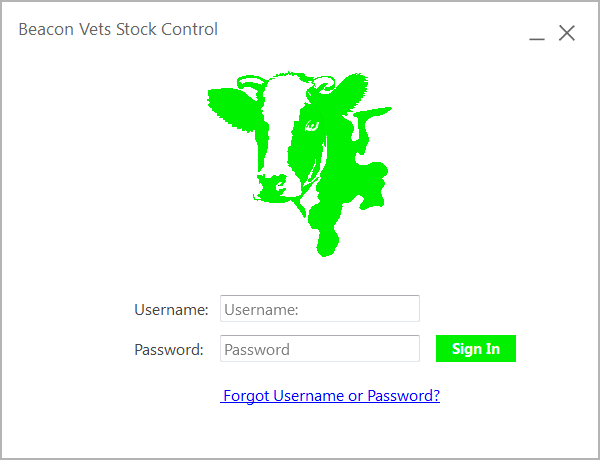
\includegraphics[width=8cm]{./ManualImages/log-in-1.png}
  
For instructions on how to run the system, go to page \pageref{fig:Running the System}.

\textbf{2.} Enter your user-name into the user-name field.

\textbf{3.} Enter your password into the password field.

If you cannot remember your user-name or password, go to page \pageref{fig:Forgetting Your User-name or Password}

\textbf{4.} Click the sign in button, if your log in details are correct you will be taken to the Current Order screen.

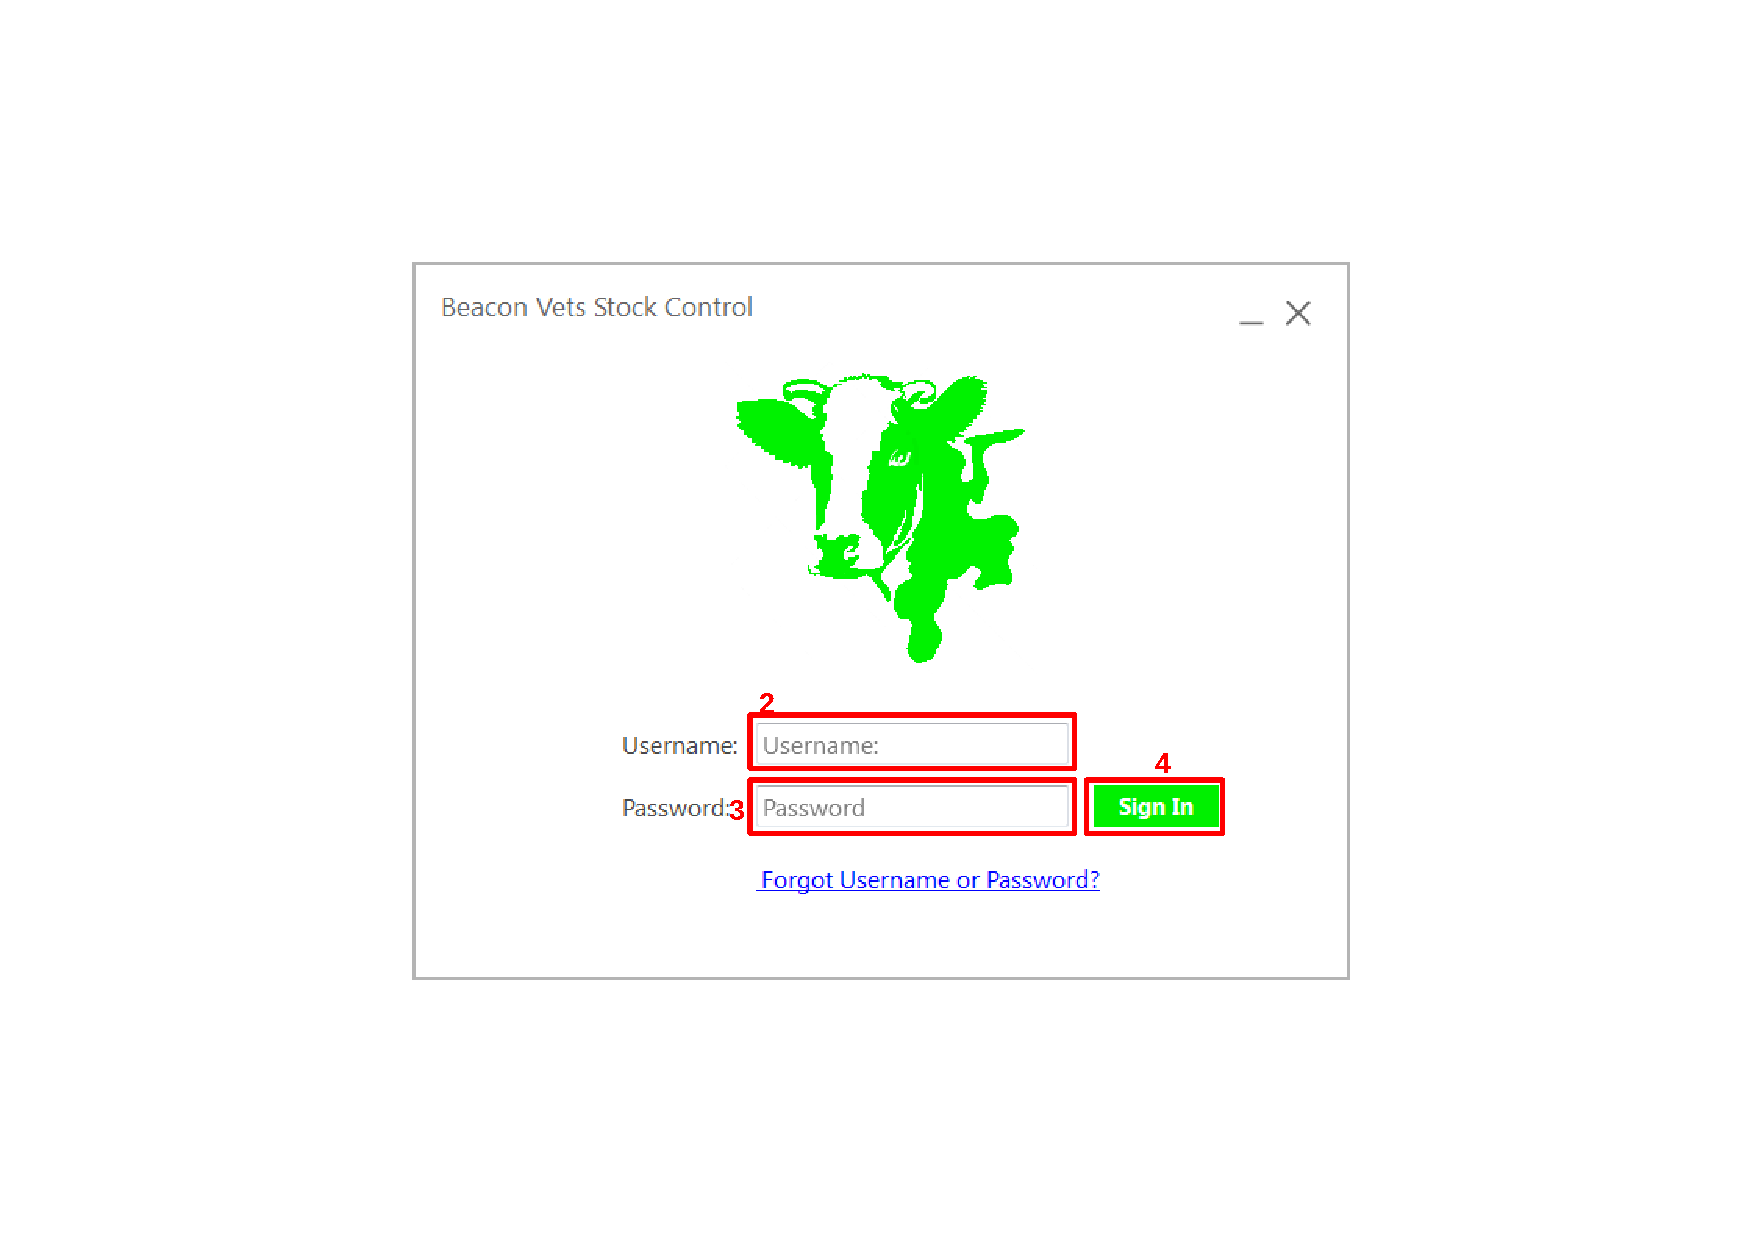
\includegraphics[width=8cm]{./ManualImages/log-in-2.pdf}

\pagebreak
\subsubsection{Logging out of the system}
\label{fig:Logging out of the system}

In order to log out of the system, you must already be logged into the system. For instructions on how to log into the system, go to page \pageref{fig:Logging into the system}.

\textbf{1.}  On any interface, Click on the `Options' button in the menu bar at the top of the page.

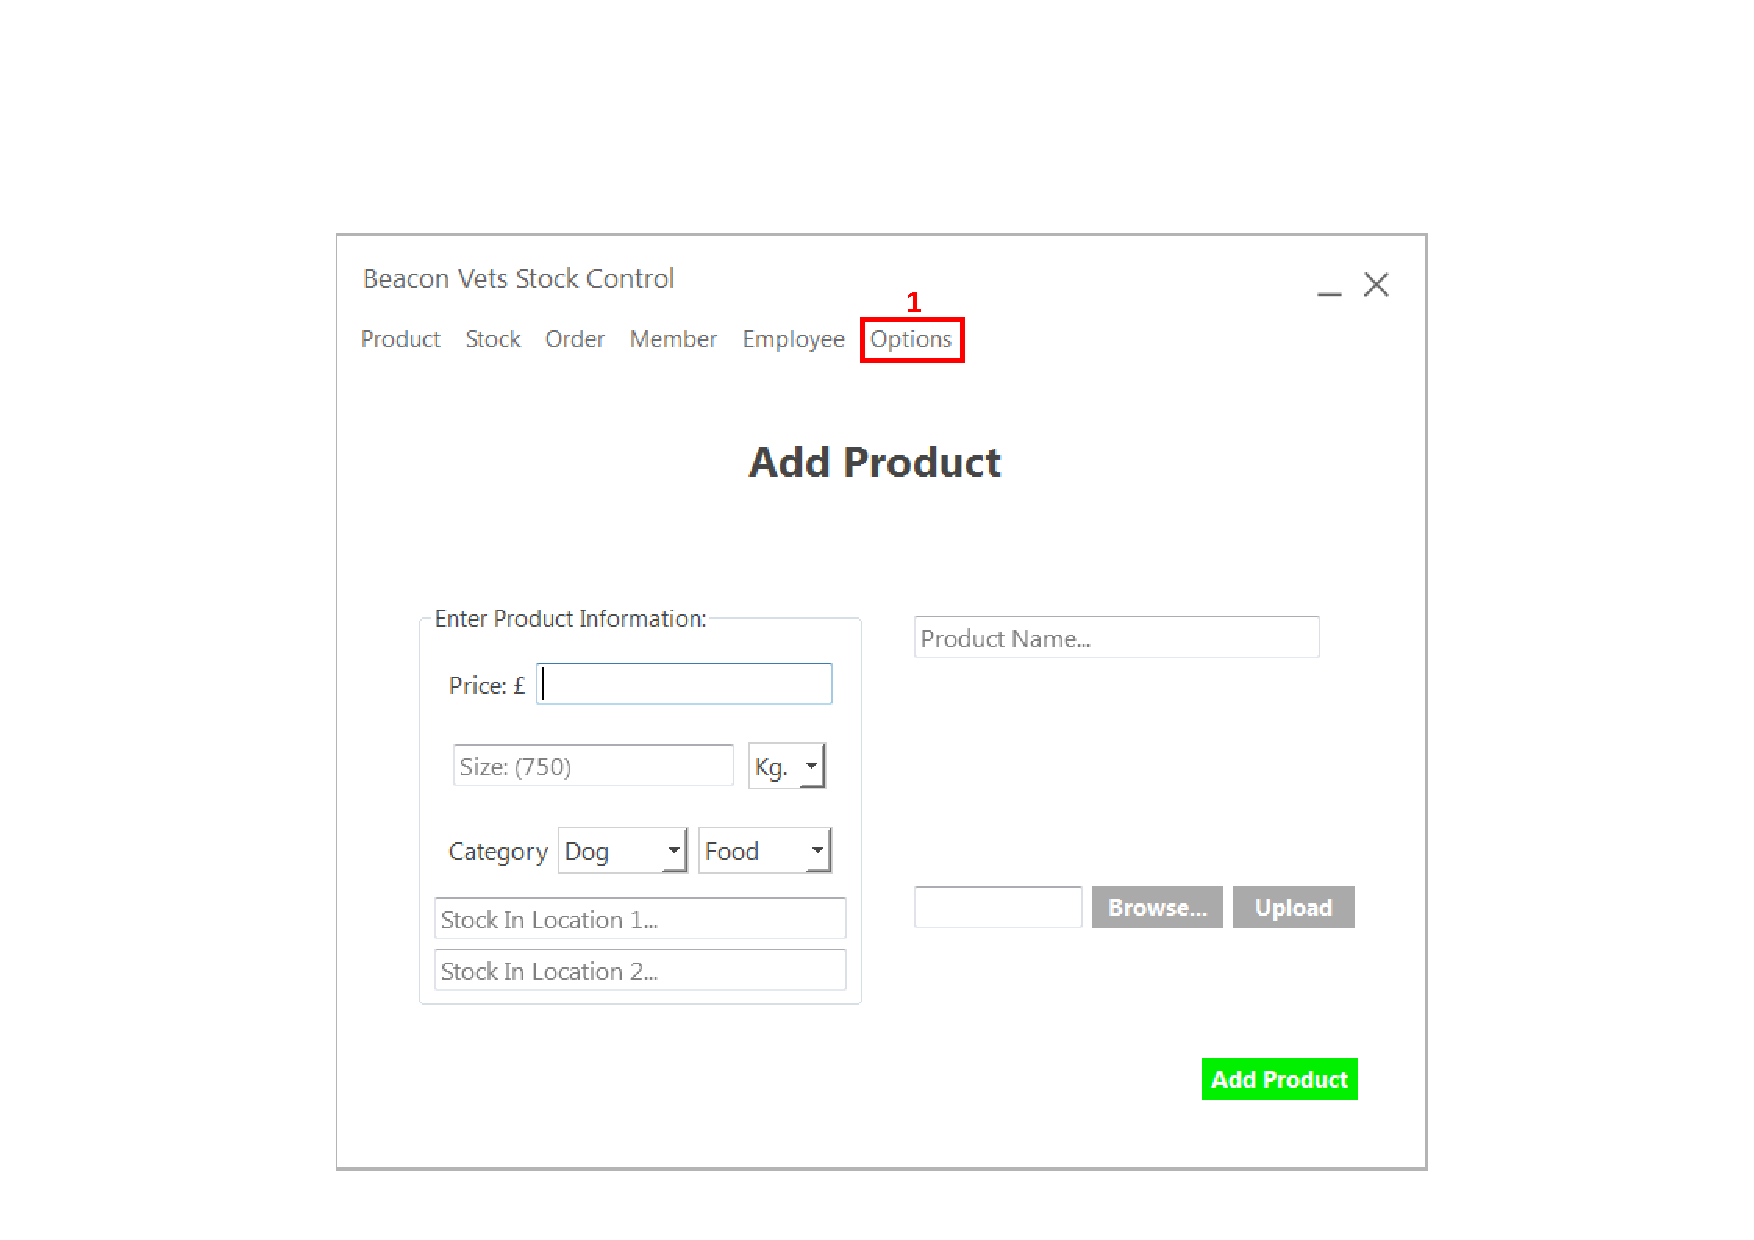
\includegraphics[width=8cm]{./ManualImages/log-off-1.pdf}

\textbf{2.} Clicking on the `Options' button will display a drop down menu. Click on the `Log Off' option from this menu.

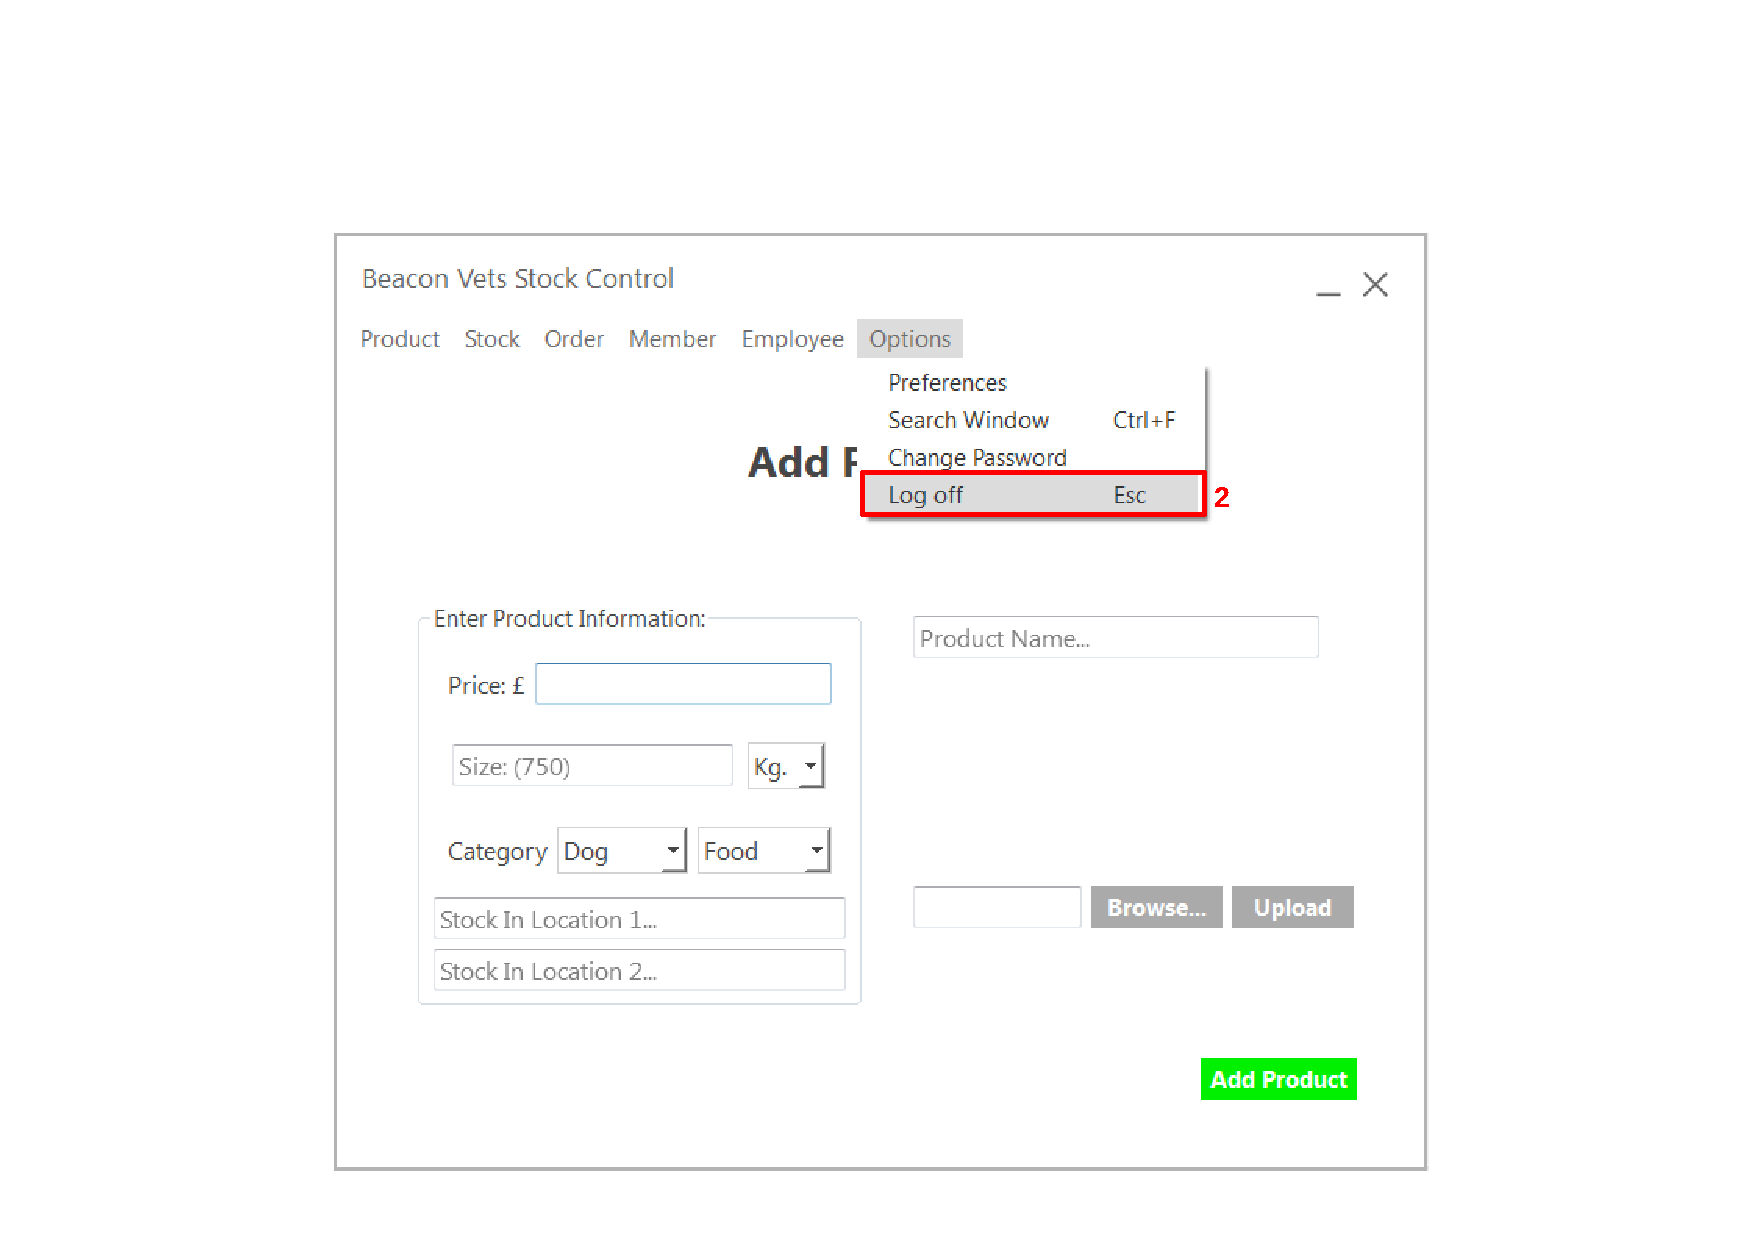
\includegraphics[width=8cm]{./ManualImages/log-off-2.pdf}

An alternative to Step 1 and Step 2 is that you can press the `ESC' button on the keyboard whilst on any interface.

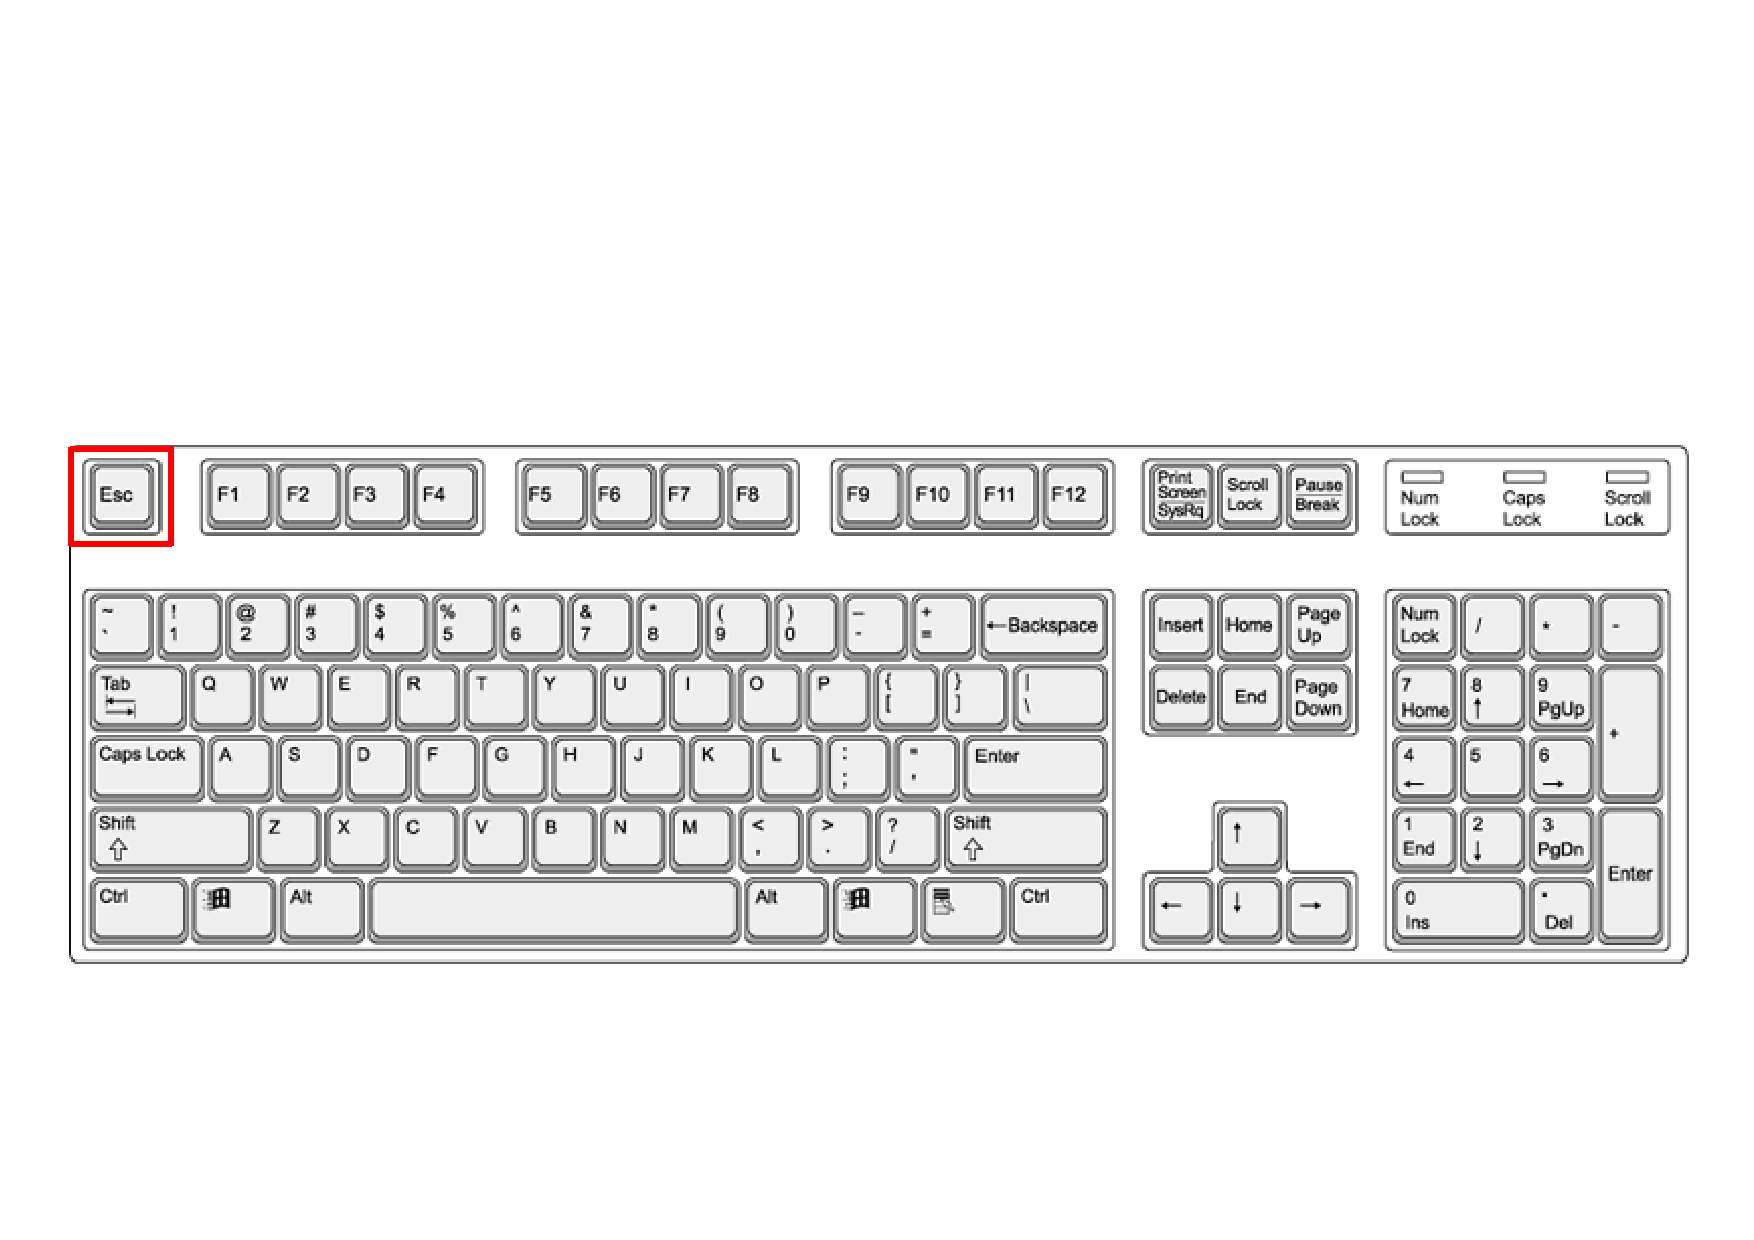
\includegraphics[width=\textwidth]{./ManualImages/shortcut-esc.pdf}

\textbf{3.} A Confirmation window will display. Click the `Yes' button.

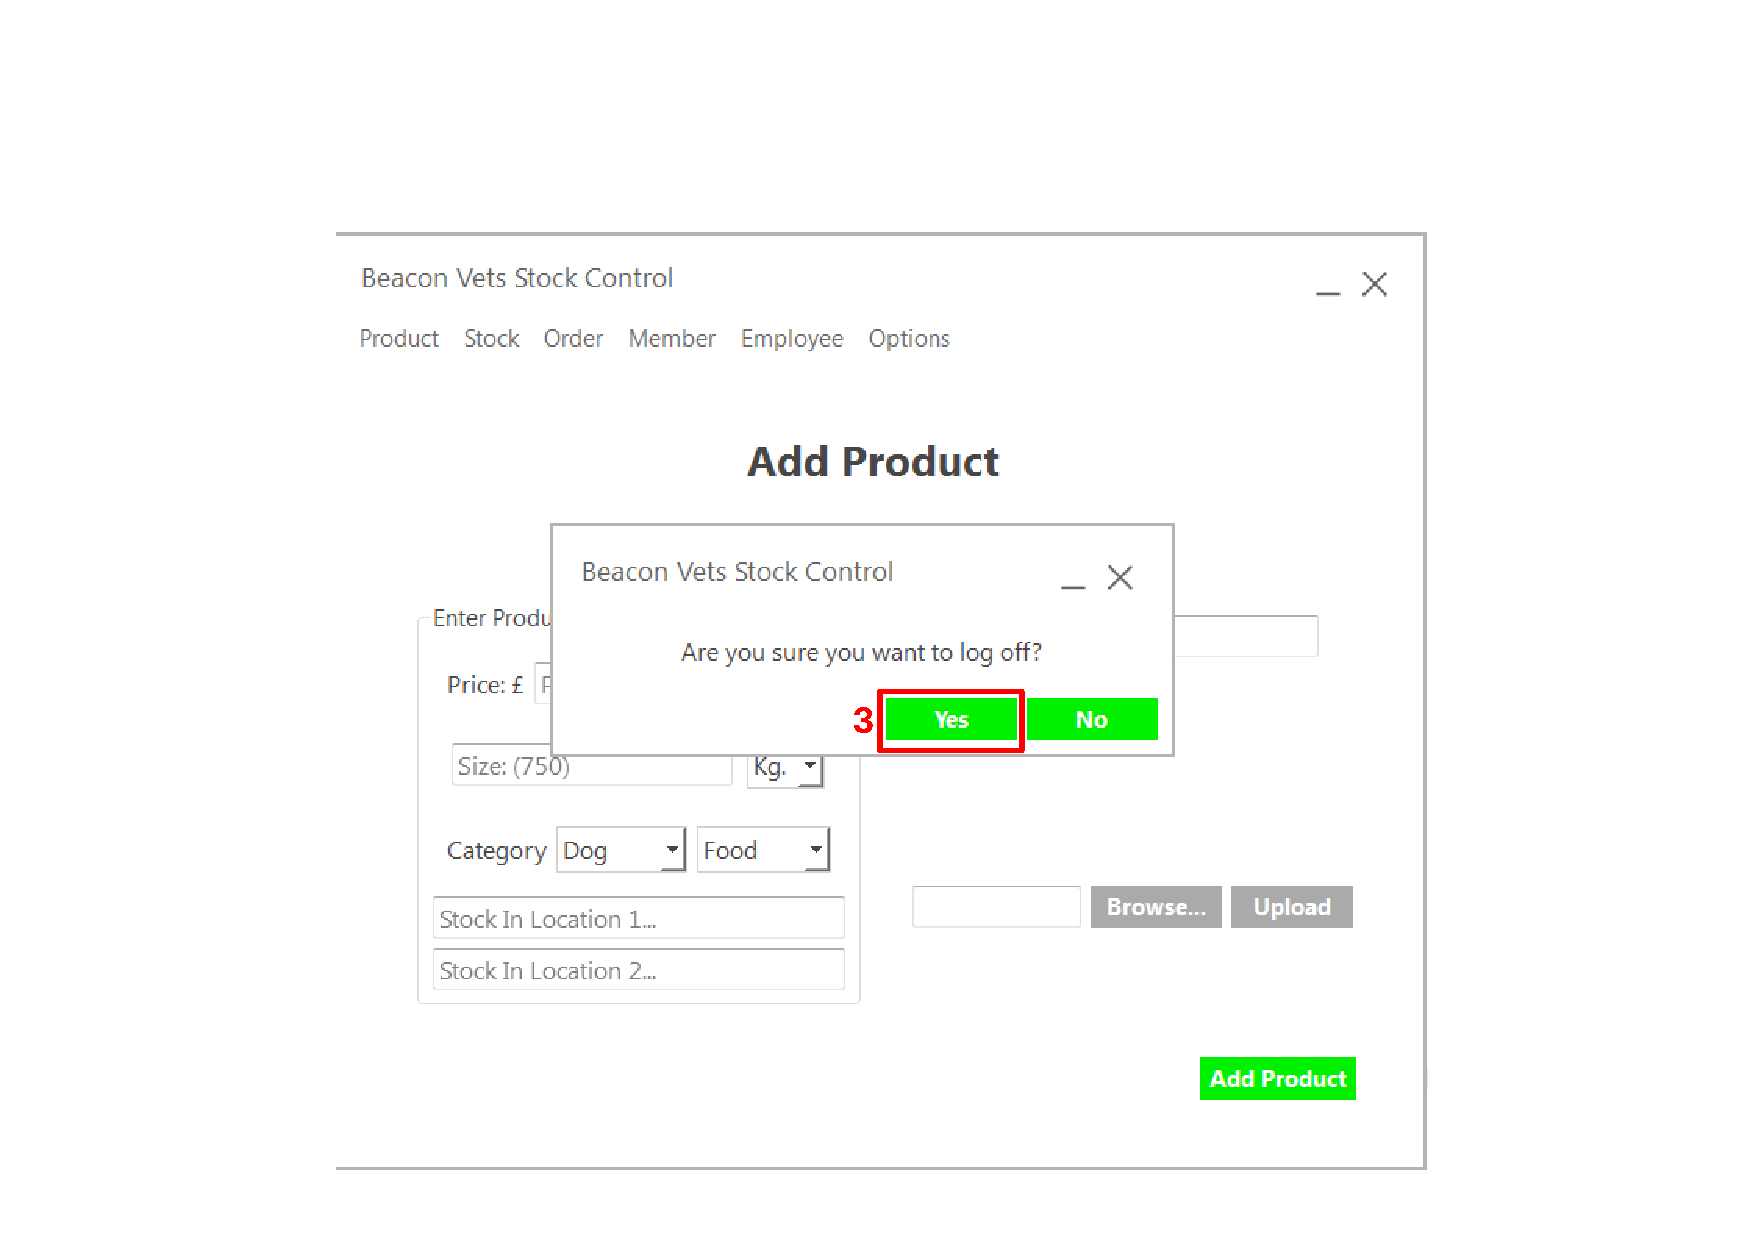
\includegraphics[width=8cm]{./ManualImages/log-off-3.pdf}

You have now logged off the system.

\pagebreak
\subsubsection{Forgetting Your User-name or Password}
\label{fig:Forgetting Your User-name or Password}

\textbf{1.} Go to the log in interface.

If you are currently logged in and do not know how to log out, go to page \pageref{fig:Logging out of the system}  for a tutorial on logging out.

\textbf{2.} Click on the `Forgot User-name or Password?' text.

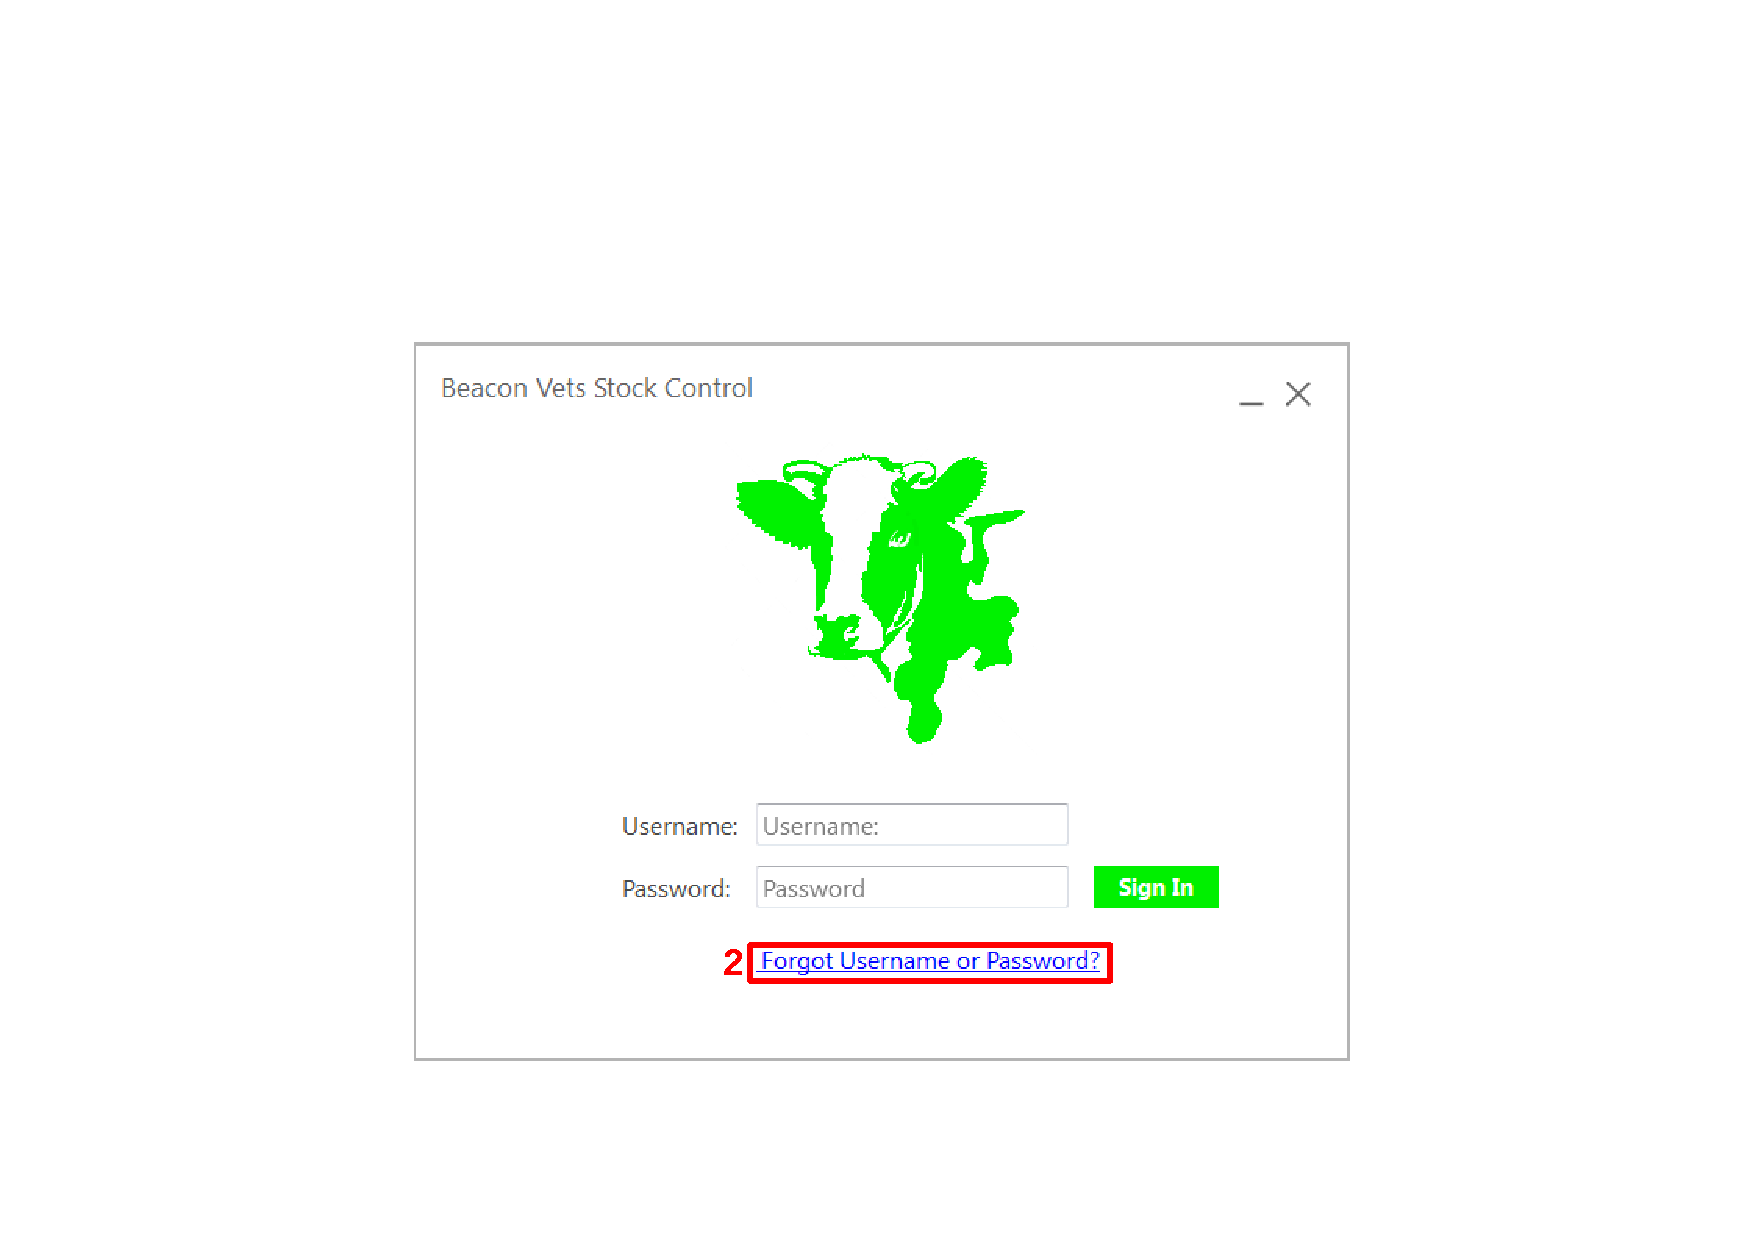
\includegraphics[width=8cm]{./ManualImages/forgot-password-1.pdf}

this will take you to the forgot password screen.

\textbf{3.} Enter the email address associated with your account.

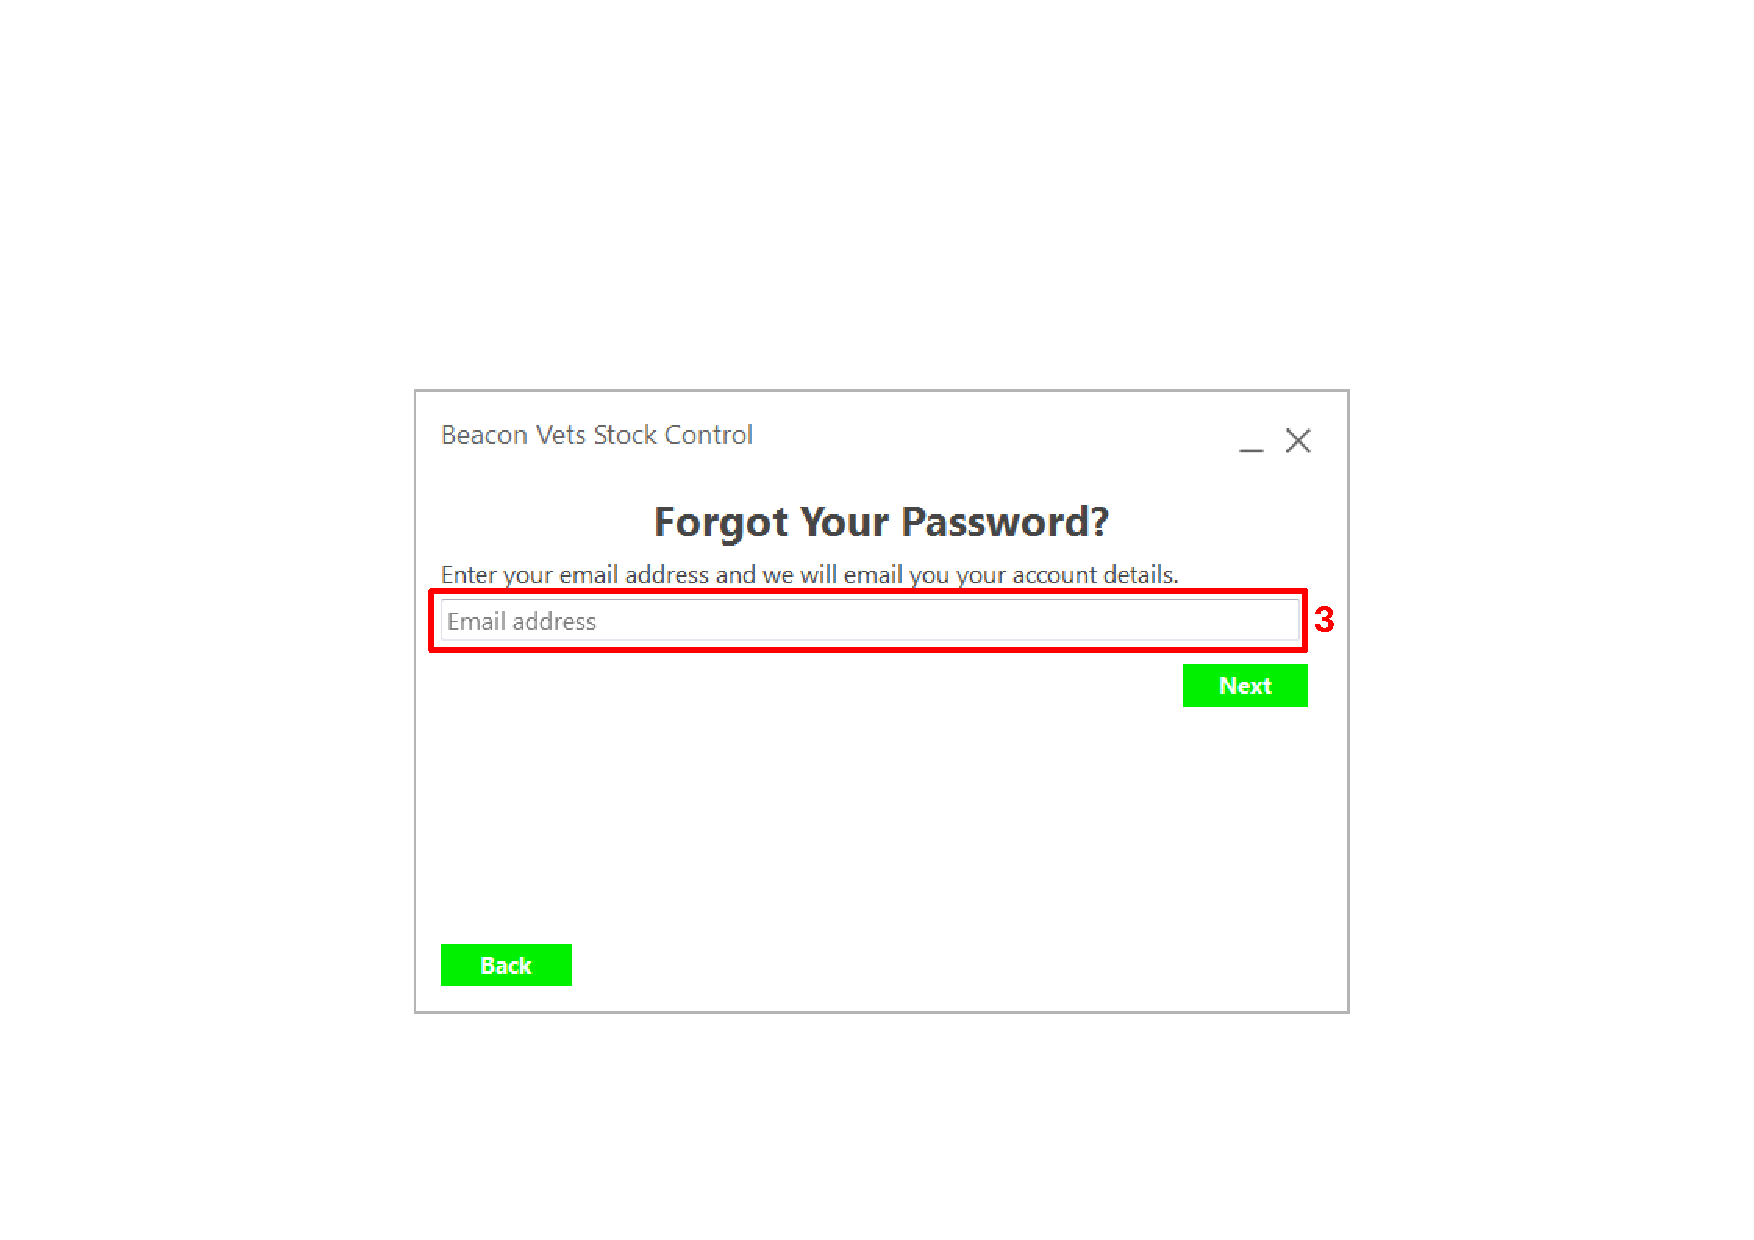
\includegraphics[width=8cm]{./ManualImages/forgot-password-2.pdf}

If you cannot remember the email address associated to your account, another employee can sign in and locate the email address associated to your account by using the search window.

For a tutorial on using the search window, go to page .

\textbf{4.} Click the `Next' button.

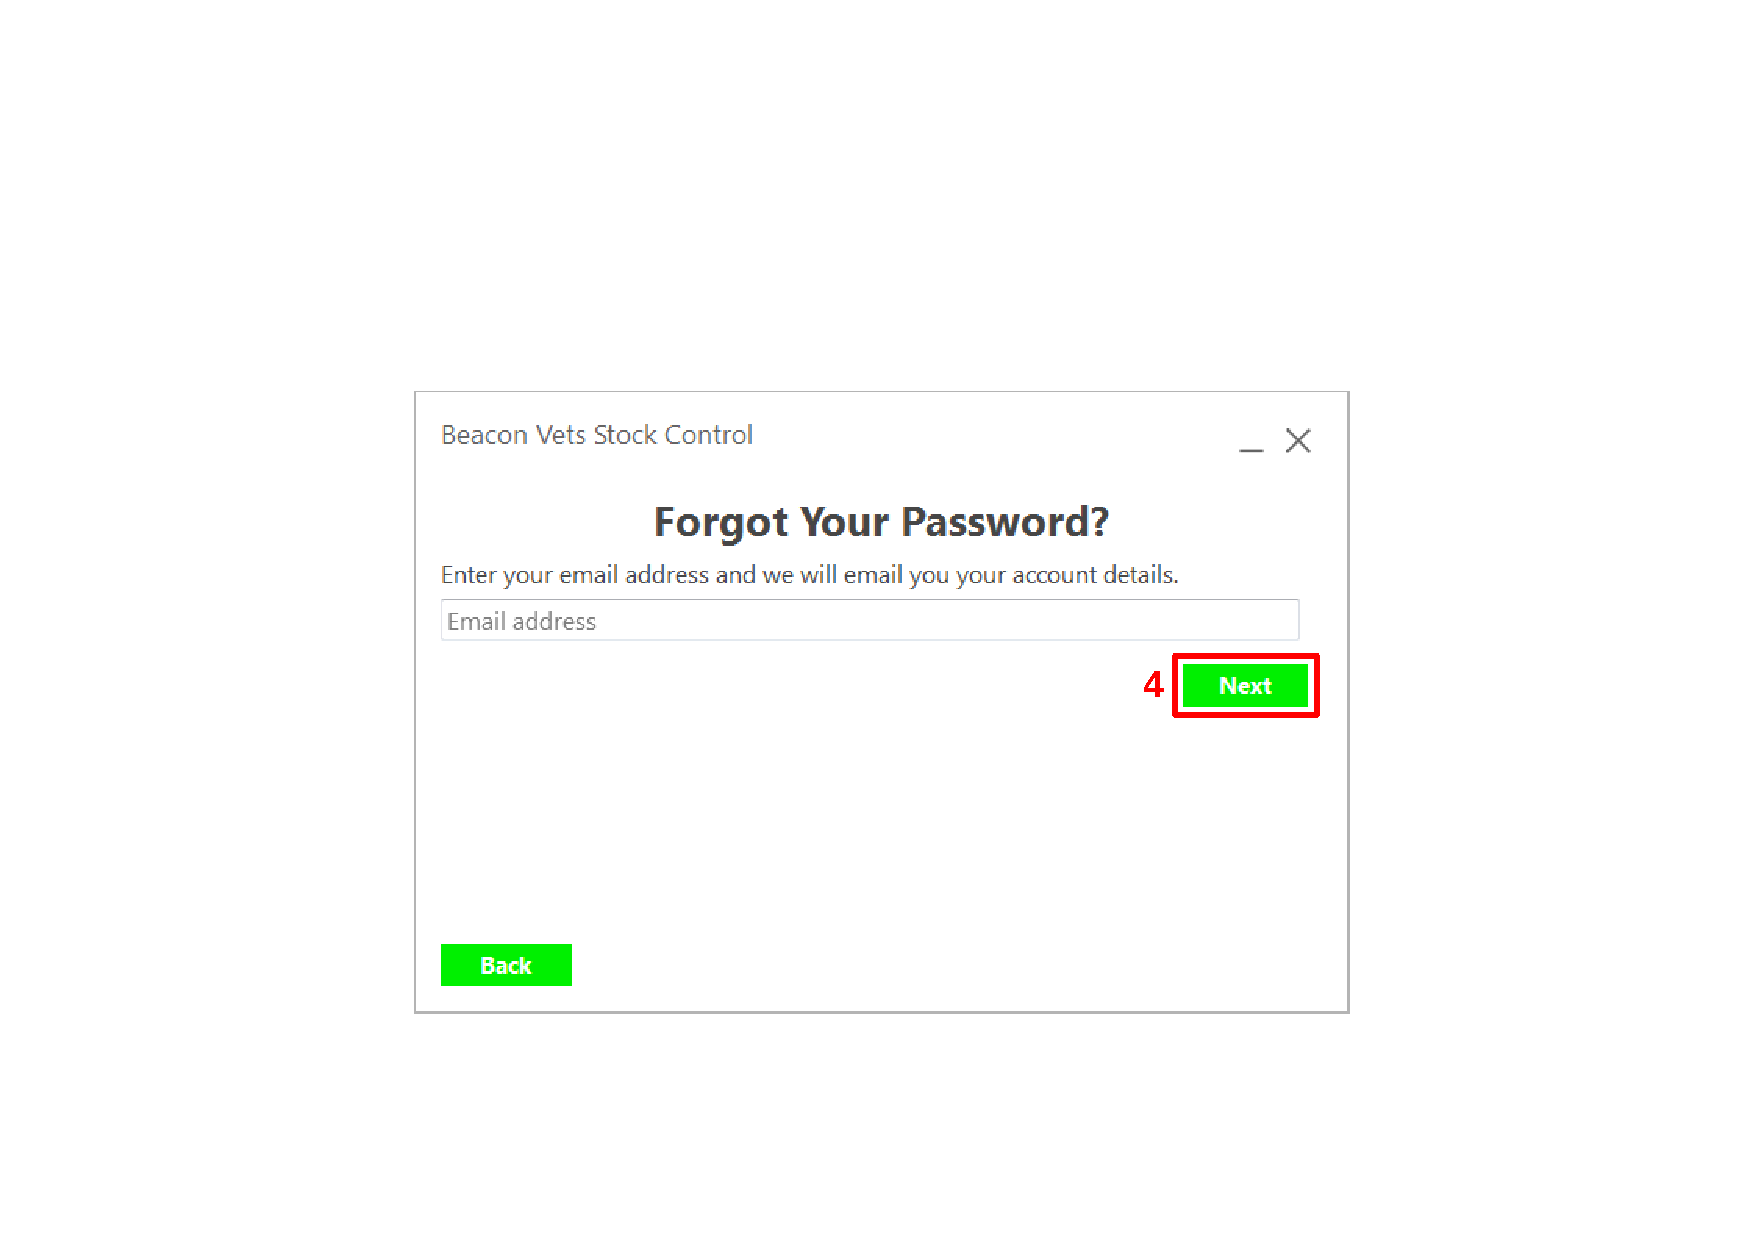
\includegraphics[width=8cm]{./ManualImages/forgot-password-3.pdf}

If the email address you entered is associated to your account, then the system will send an email to that email address, containing your user-name and password.

\textbf{5.} Check your email inbox. If you did not received the email, first check your spam or junk folder and if the email is not in there, repeat step 3 and 4.

If you can no longer access the email address associated to your account, go to page \pageref{fig:Unable to access your email address}.

\pagebreak
\subsubsection{Unable to access your email address}
\label{fig:Unable to access your email address}

If you are unable to access the email address associated to your account, the administrator must log into their account on the system. They must then change the email address associated to your account, to one in which you do have access to. For a tutorial on how to do this, go to page \pageref{fig:Editing an Employee in the system}.

\pagebreak
\subsubsection{Adding a Product to the system}
\label{fig:Adding a Product to the system}

\textbf{1.} Log into the system.

If you do not know how to log into the system, the tutorial on how to log into the system can be found on page \pageref{fig:Logging into the system}.

\textbf{2.} On any interface, click on the product option in the menu bar.

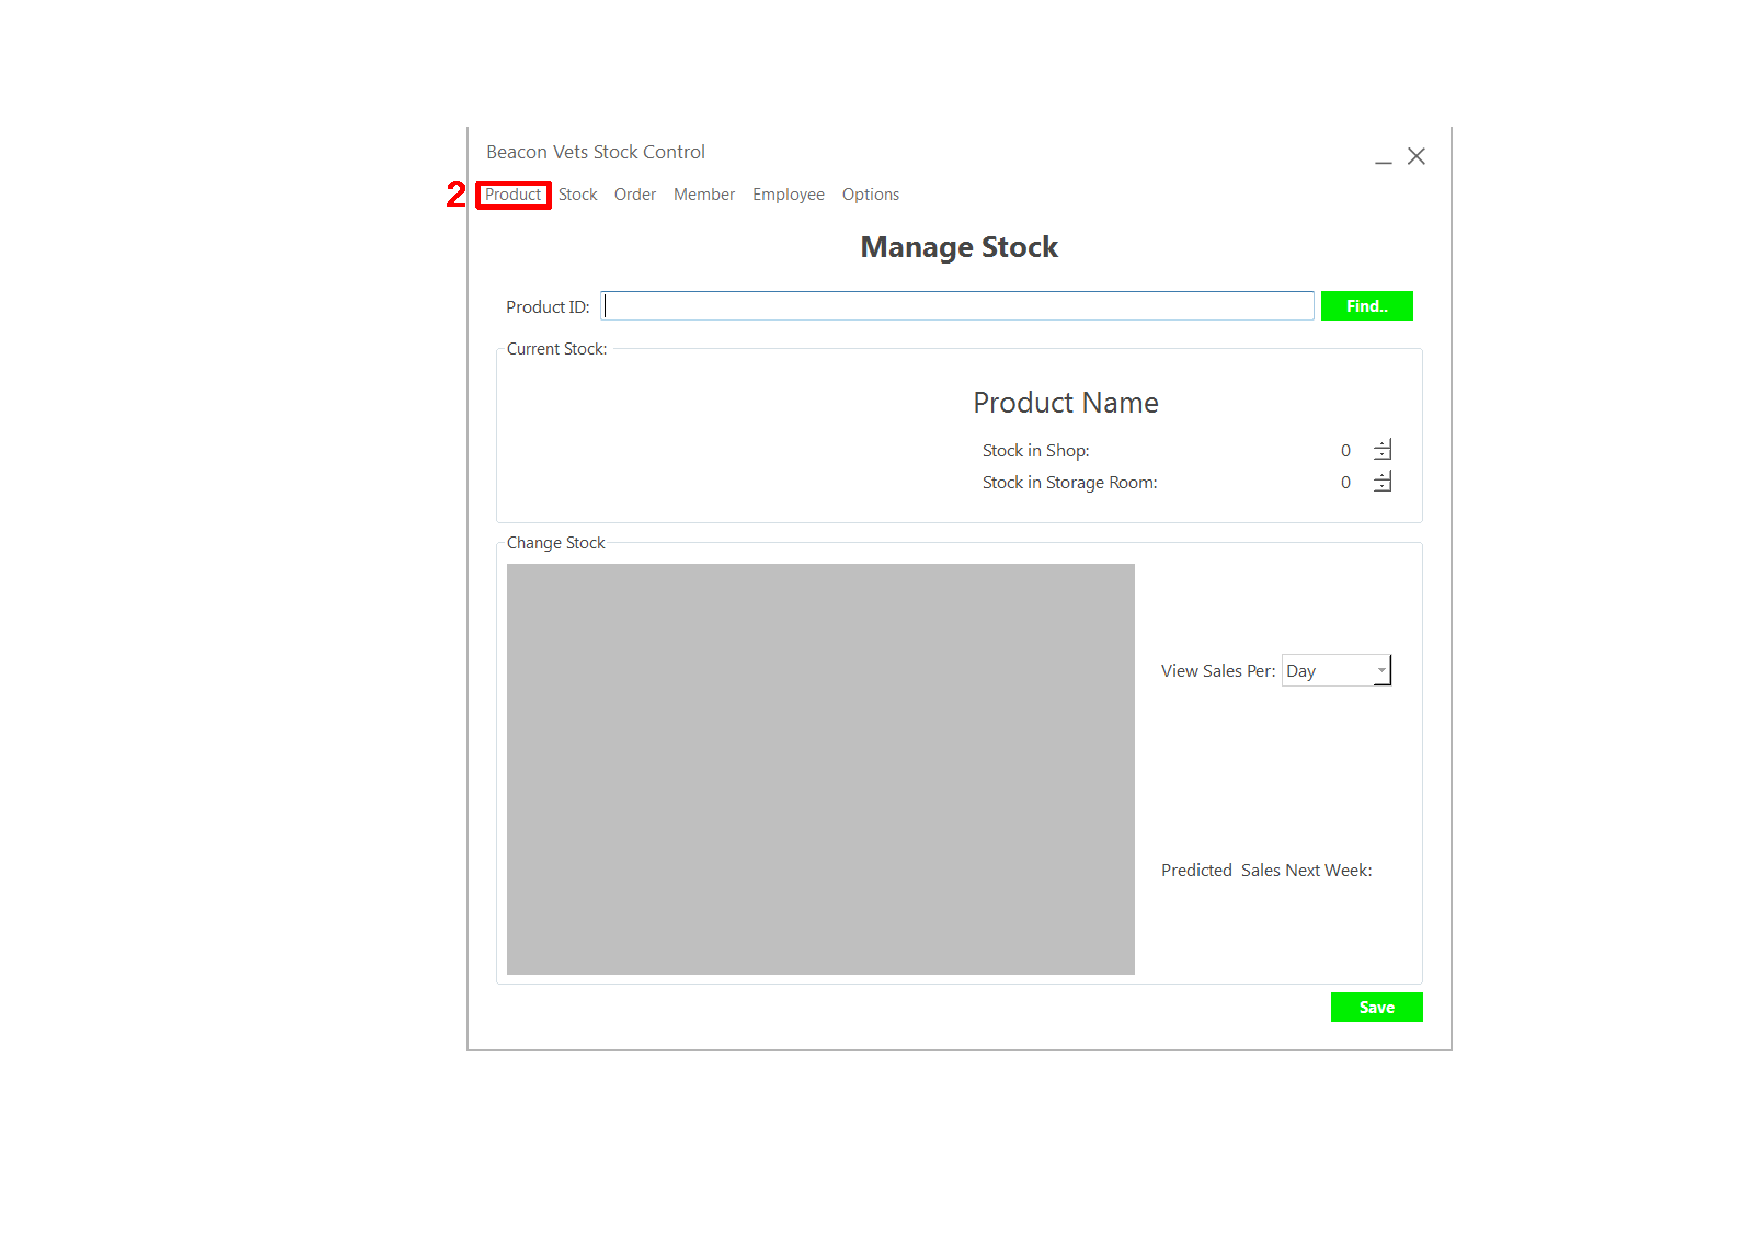
\includegraphics[width=8cm]{./ManualImages/add-product-1.pdf}

\textbf{3.} Click on the `Add a New Product' option from the drop down menu.

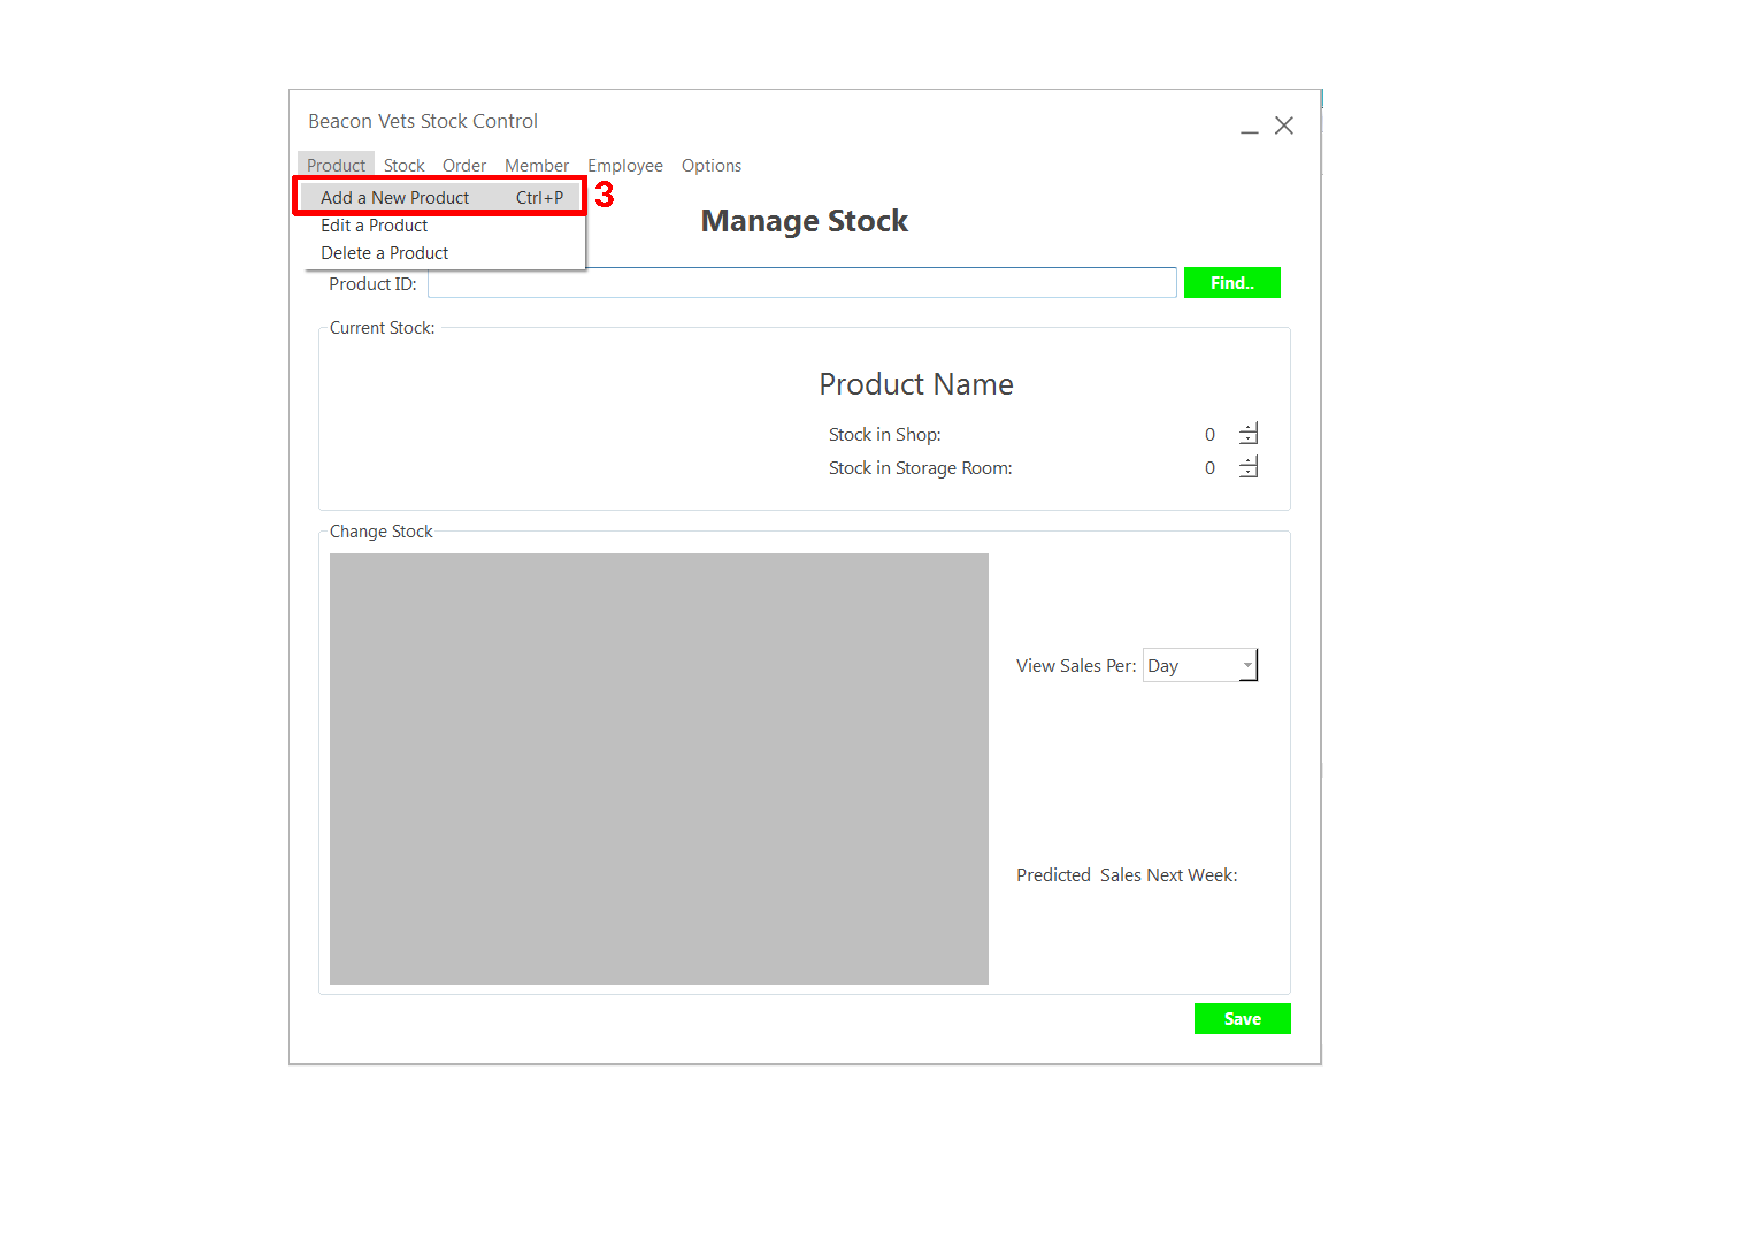
\includegraphics[width=8cm]{./ManualImages/add-product-2.pdf}

An alternative to step 2 and step 3, is by pressing the `CTRL' and `P' button on the keyboard simultaneously.

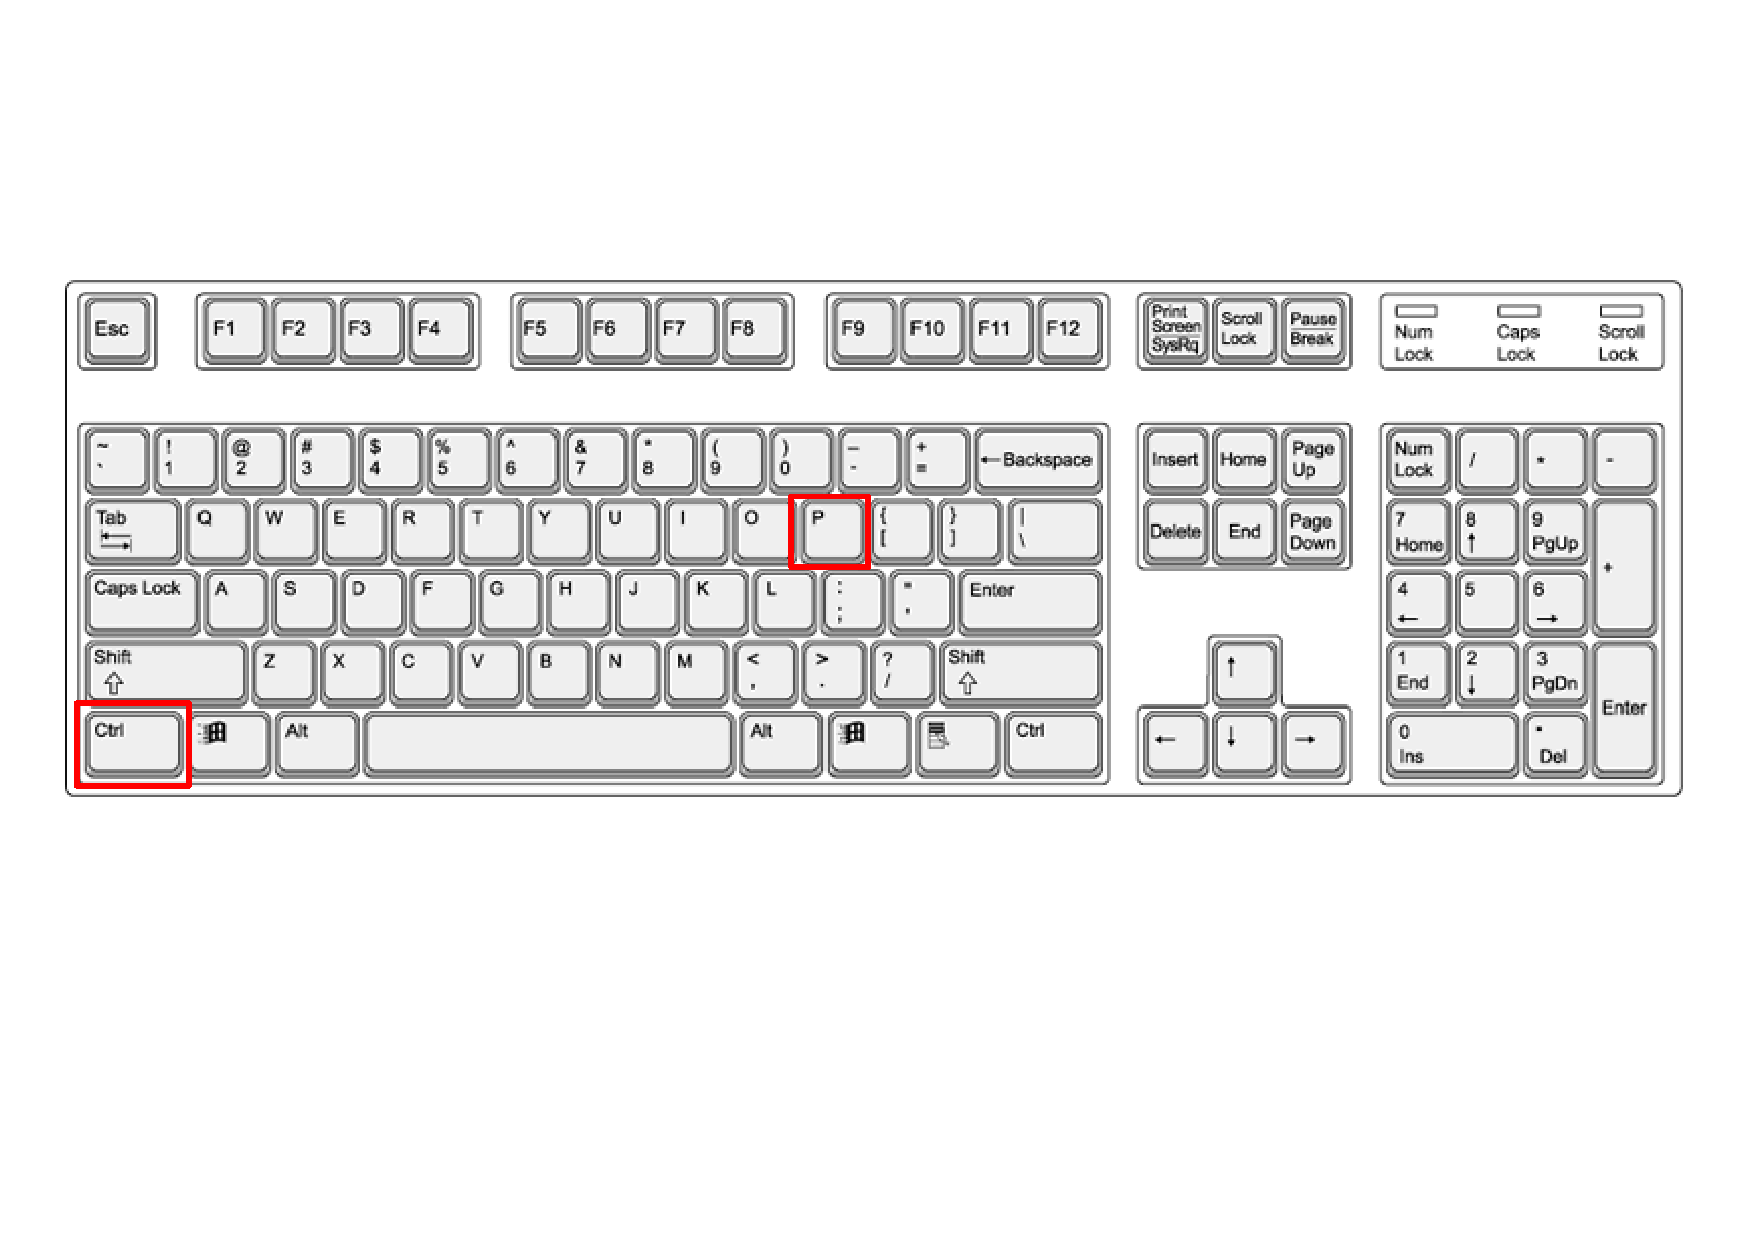
\includegraphics[width=\textwidth]{./ManualImages/shortcut-product.pdf}

\textbf{4. }Enter data into the data fields.

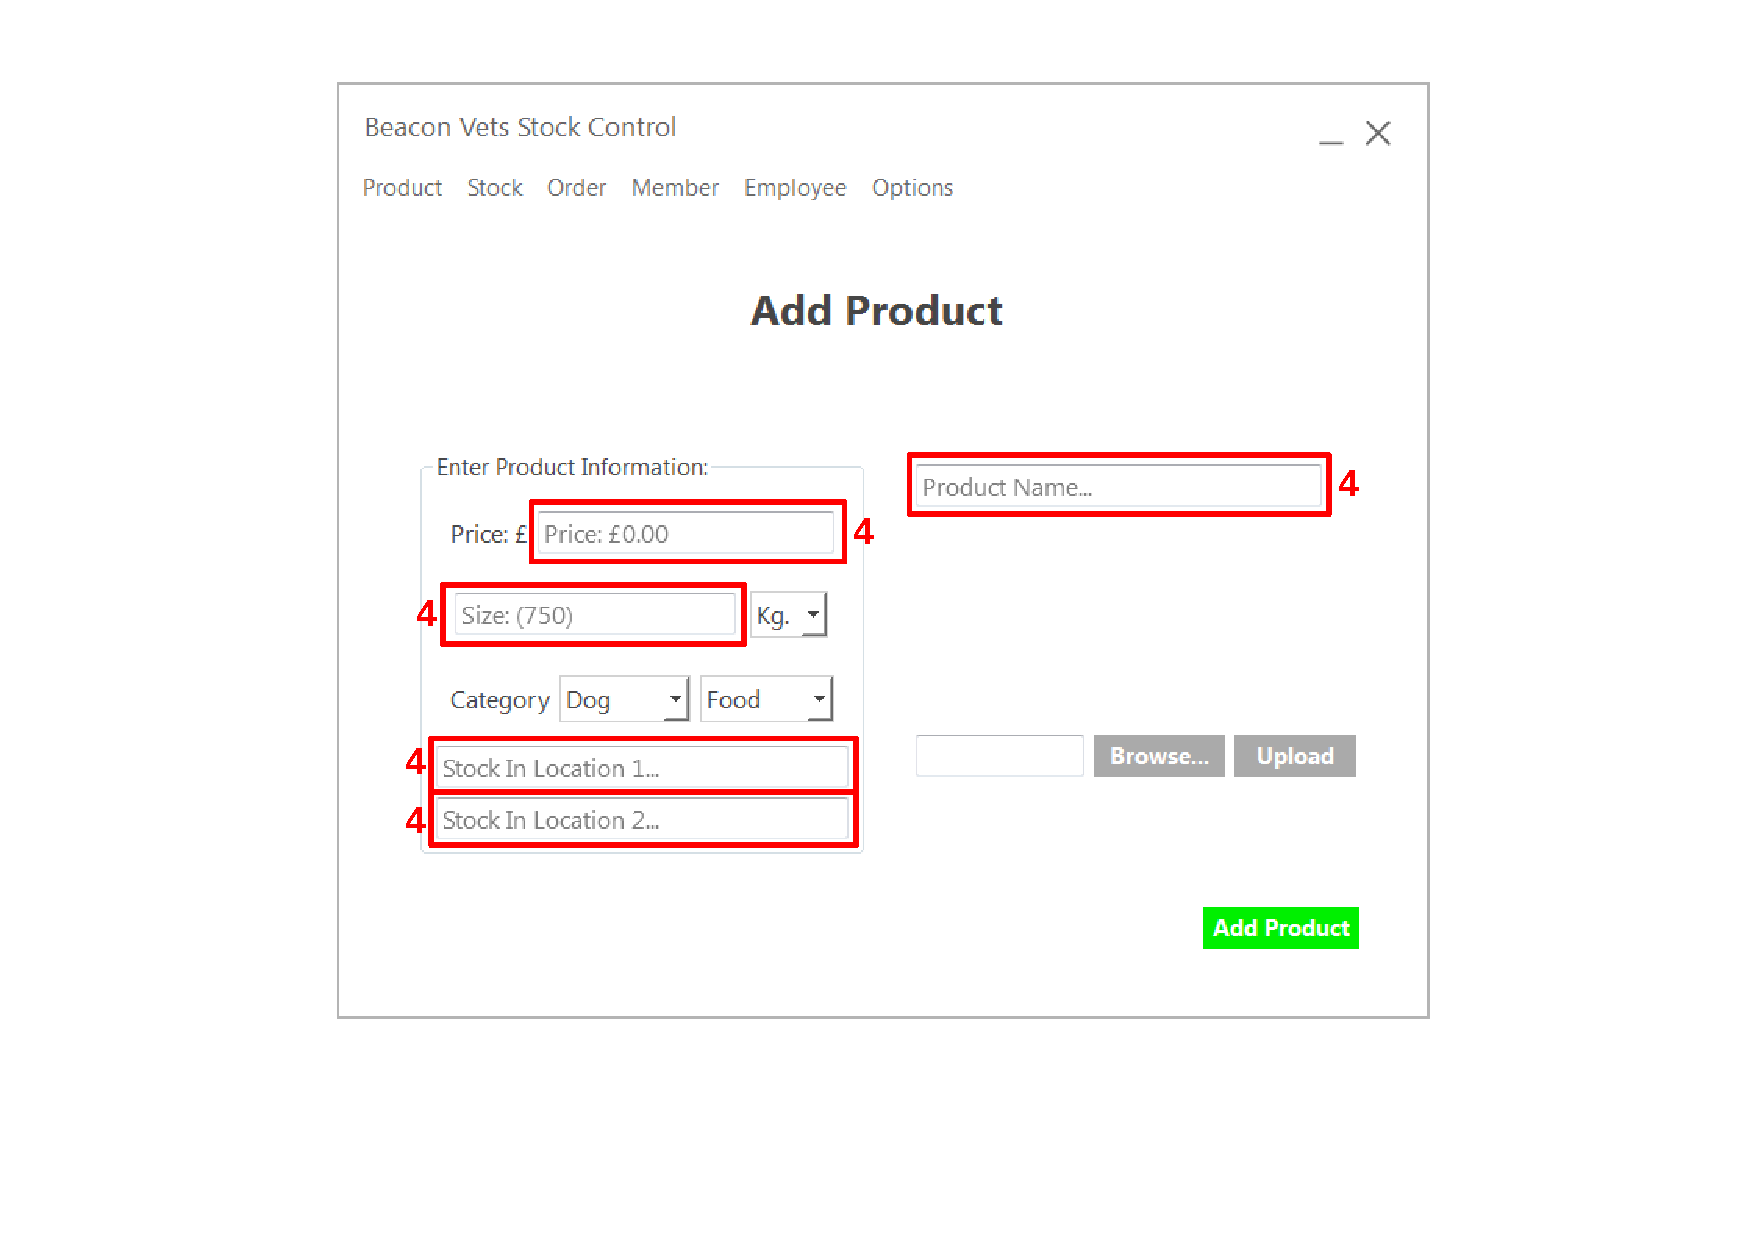
\includegraphics[width=8cm]{./ManualImages/add-product-3.pdf}

\textbf{5.} Choose the appropriate option in the drop down menus.

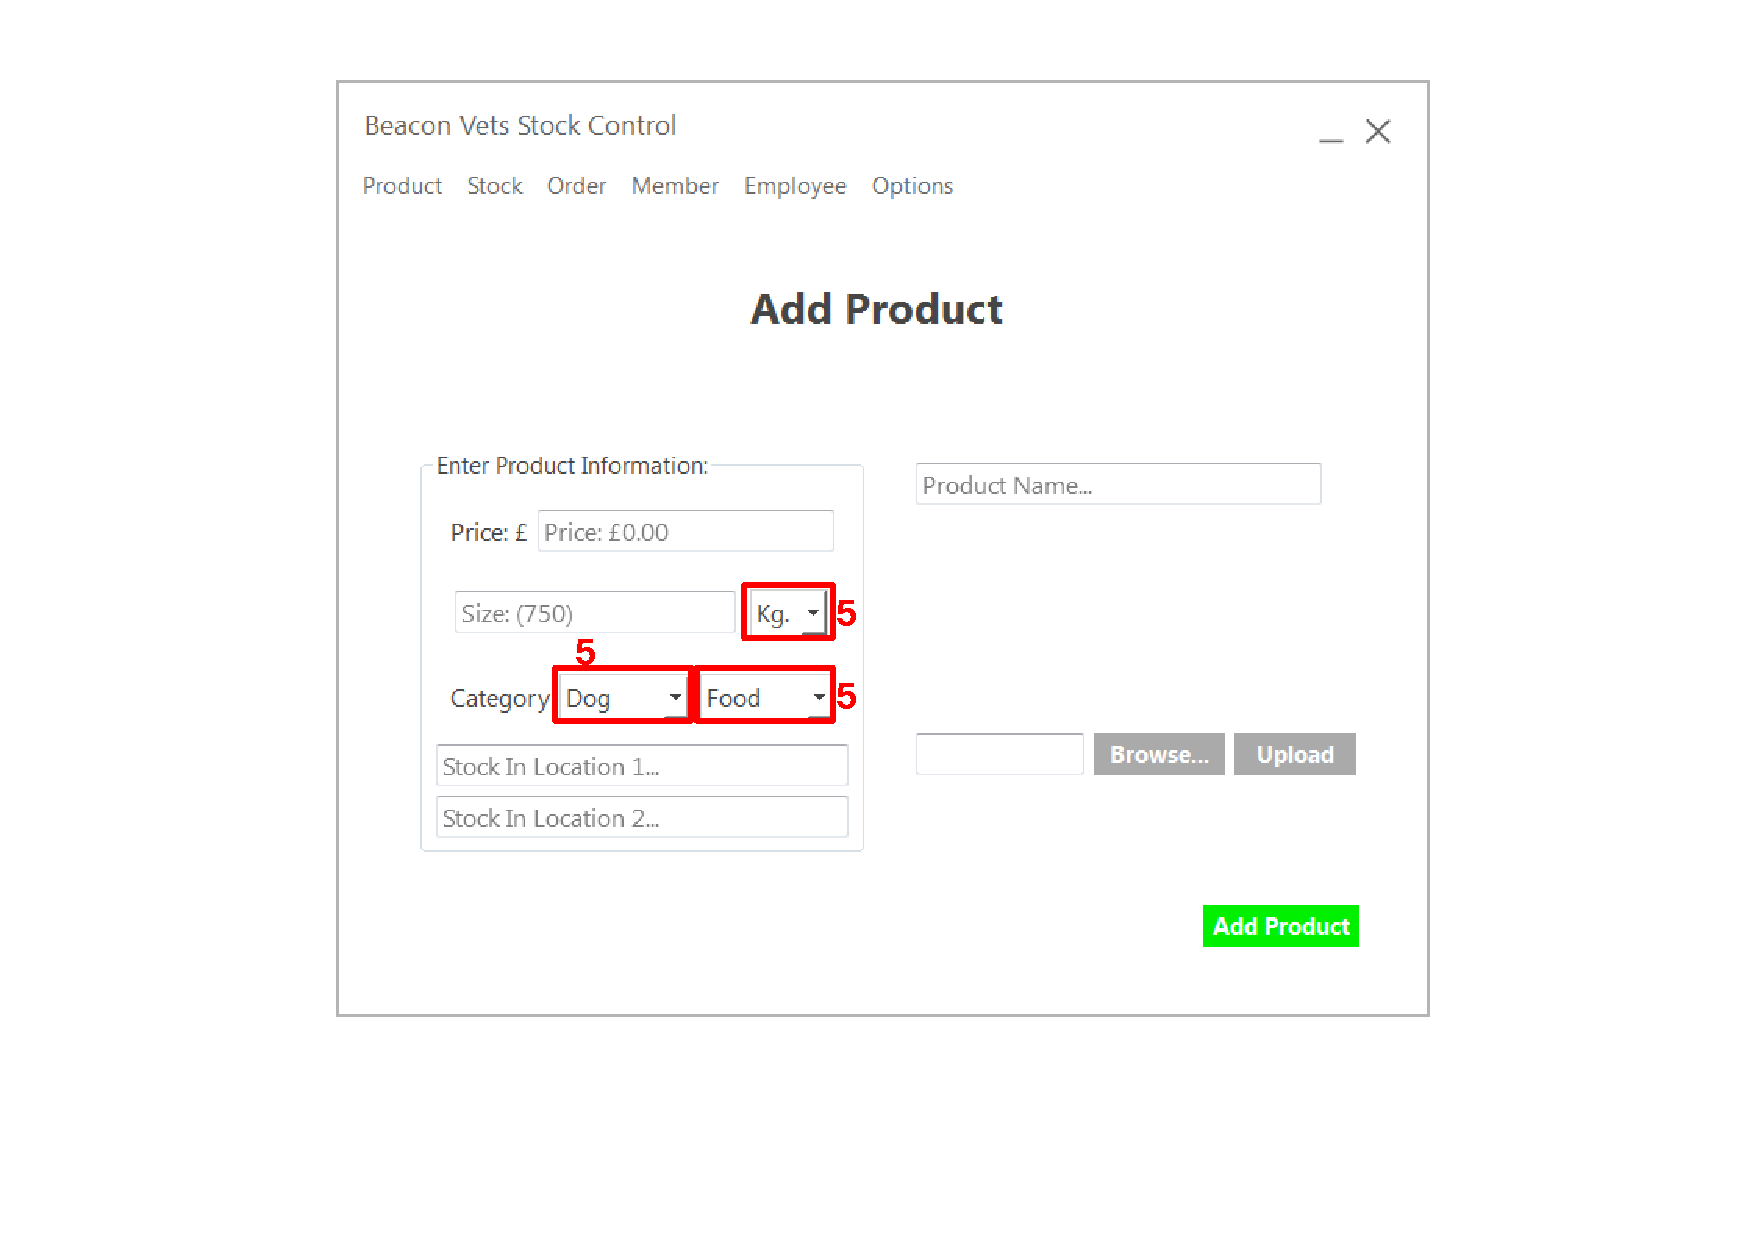
\includegraphics[width=8cm]{./ManualImages/add-product-4.pdf}

\textbf{6.} Click on the browse button.

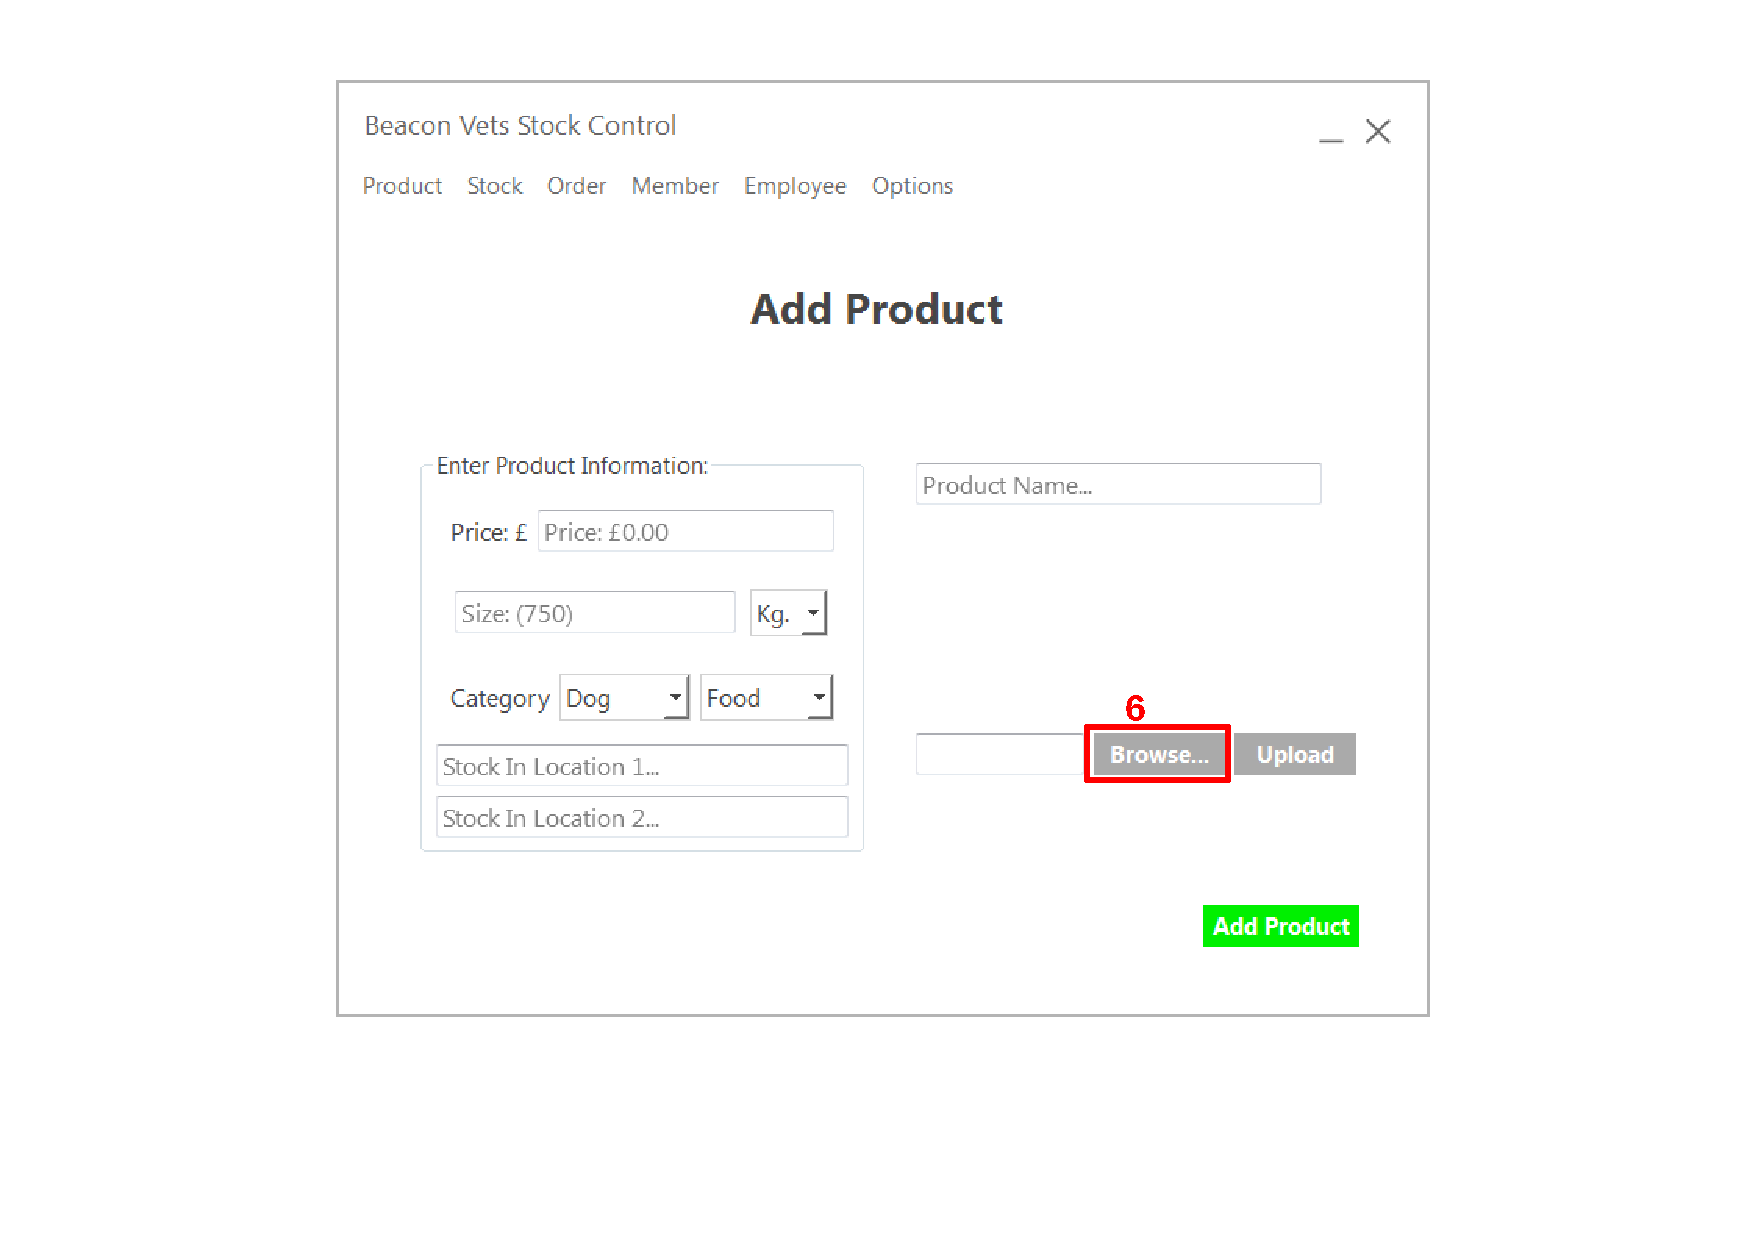
\includegraphics[width=8cm]{./ManualImages/add-product-5.pdf}

\textbf{7.} Choose an image to represent the product.

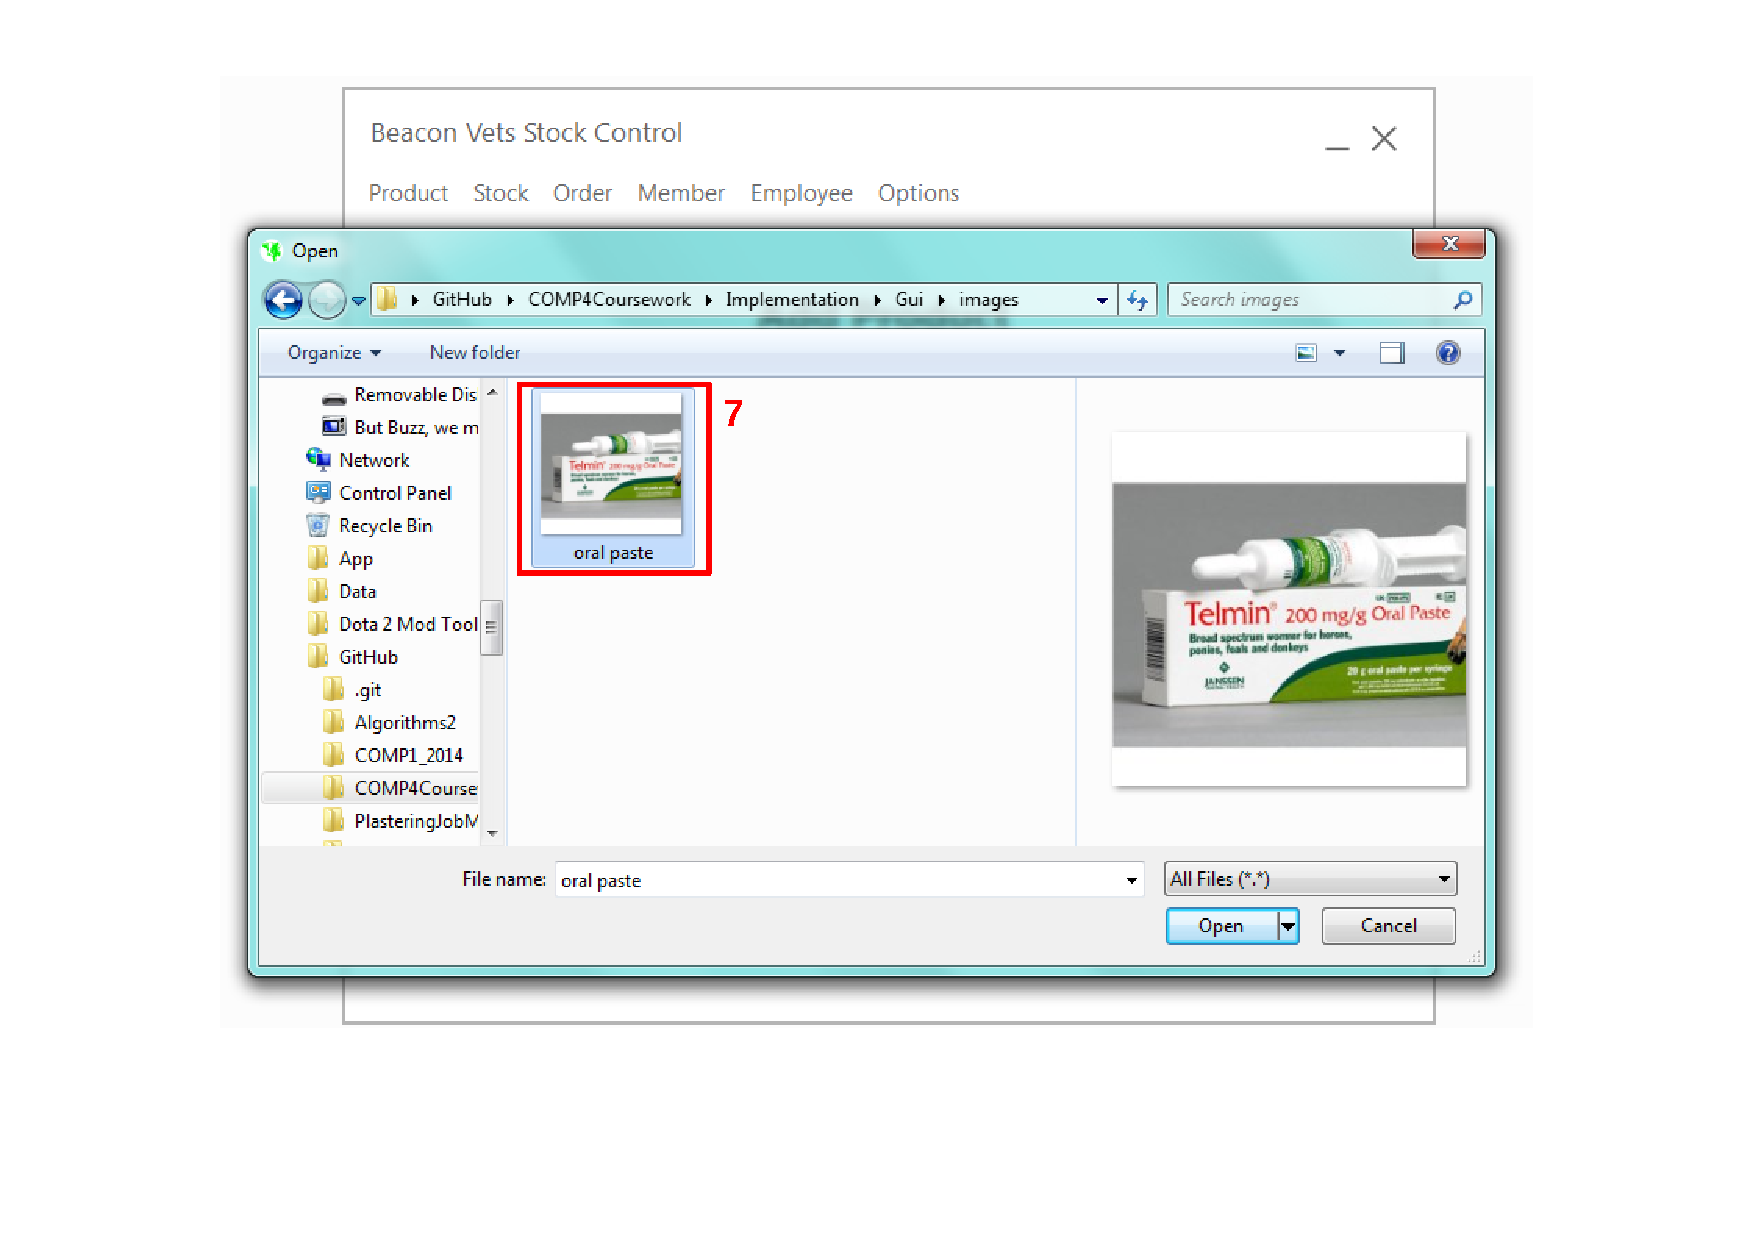
\includegraphics[width=8cm]{./ManualImages/add-product-6.pdf}

\textbf{8.} Click on the `Open' button.

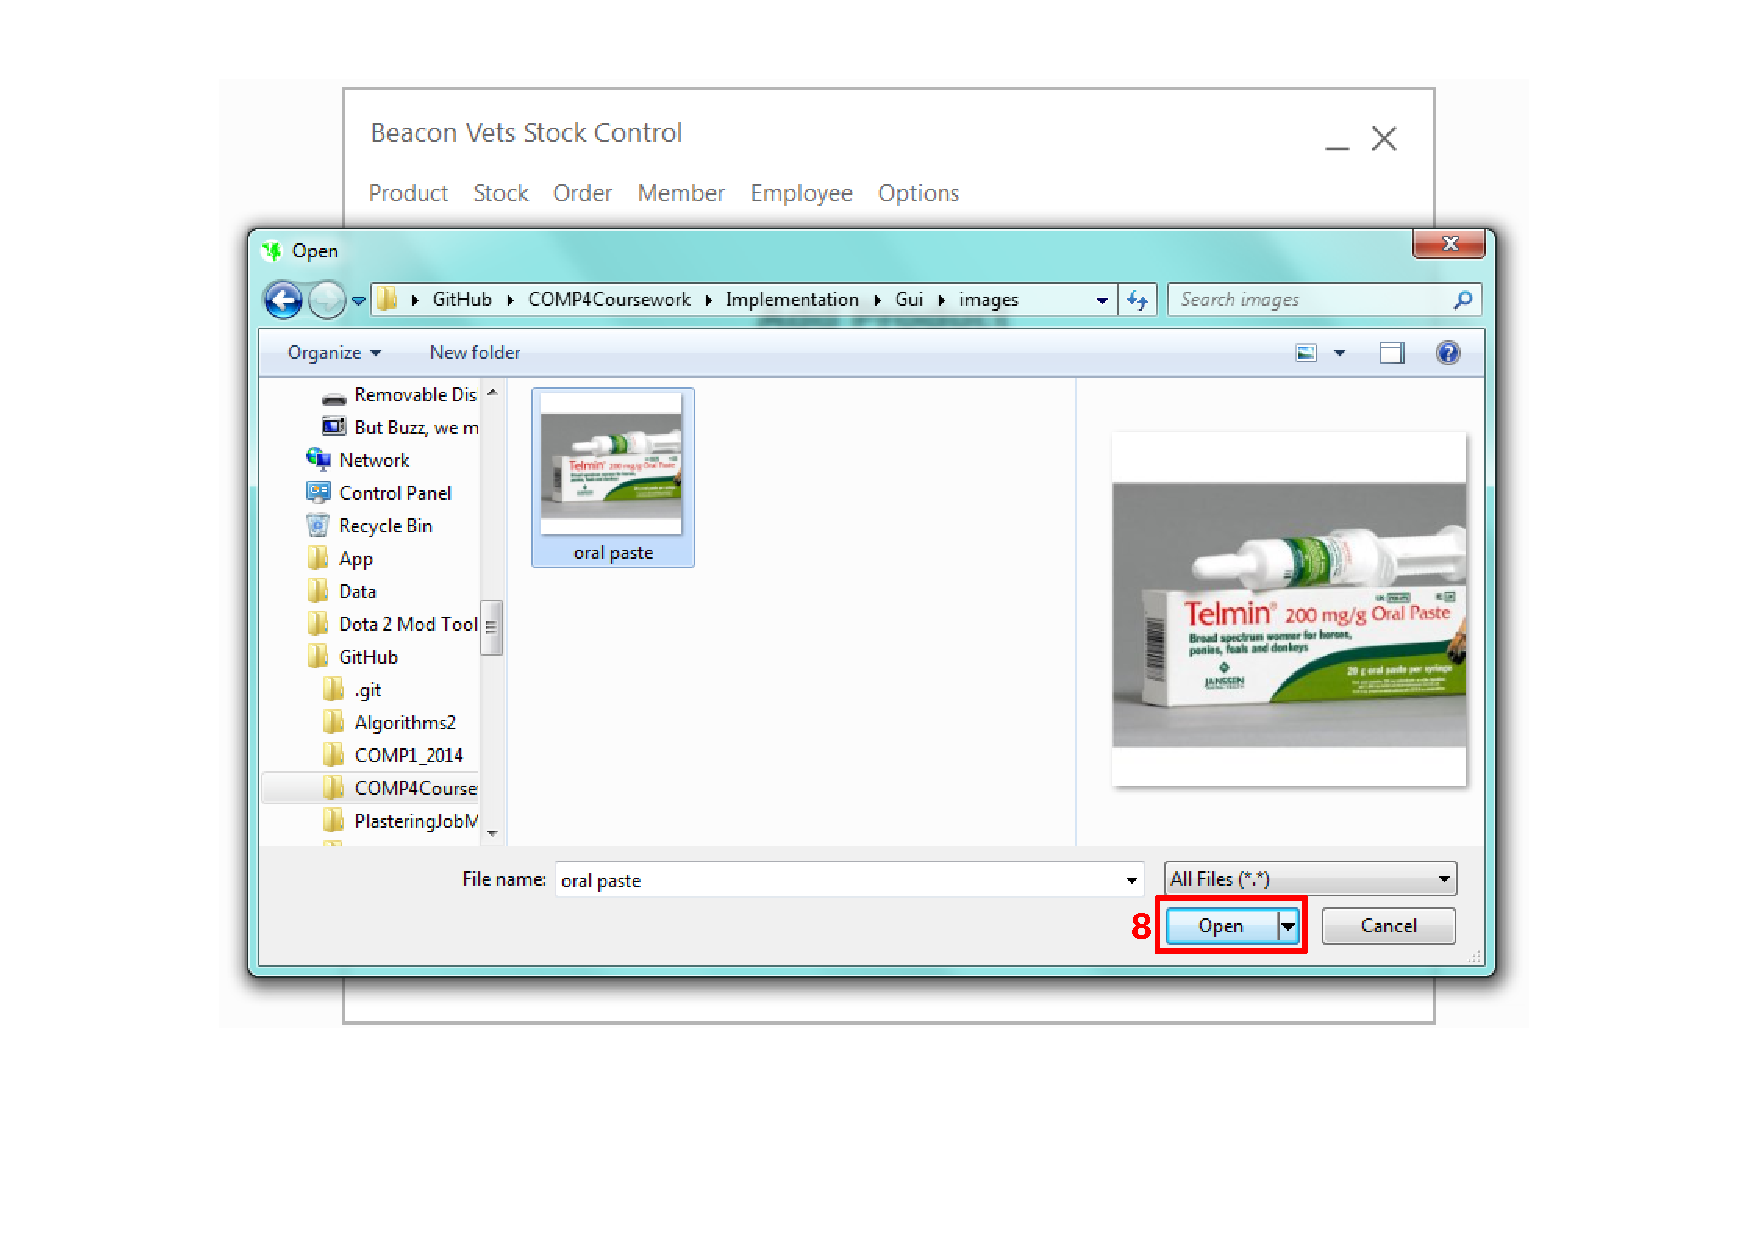
\includegraphics[width=8cm]{./ManualImages/add-product-7.pdf}

\textbf{9.} Click the `Upload' button.

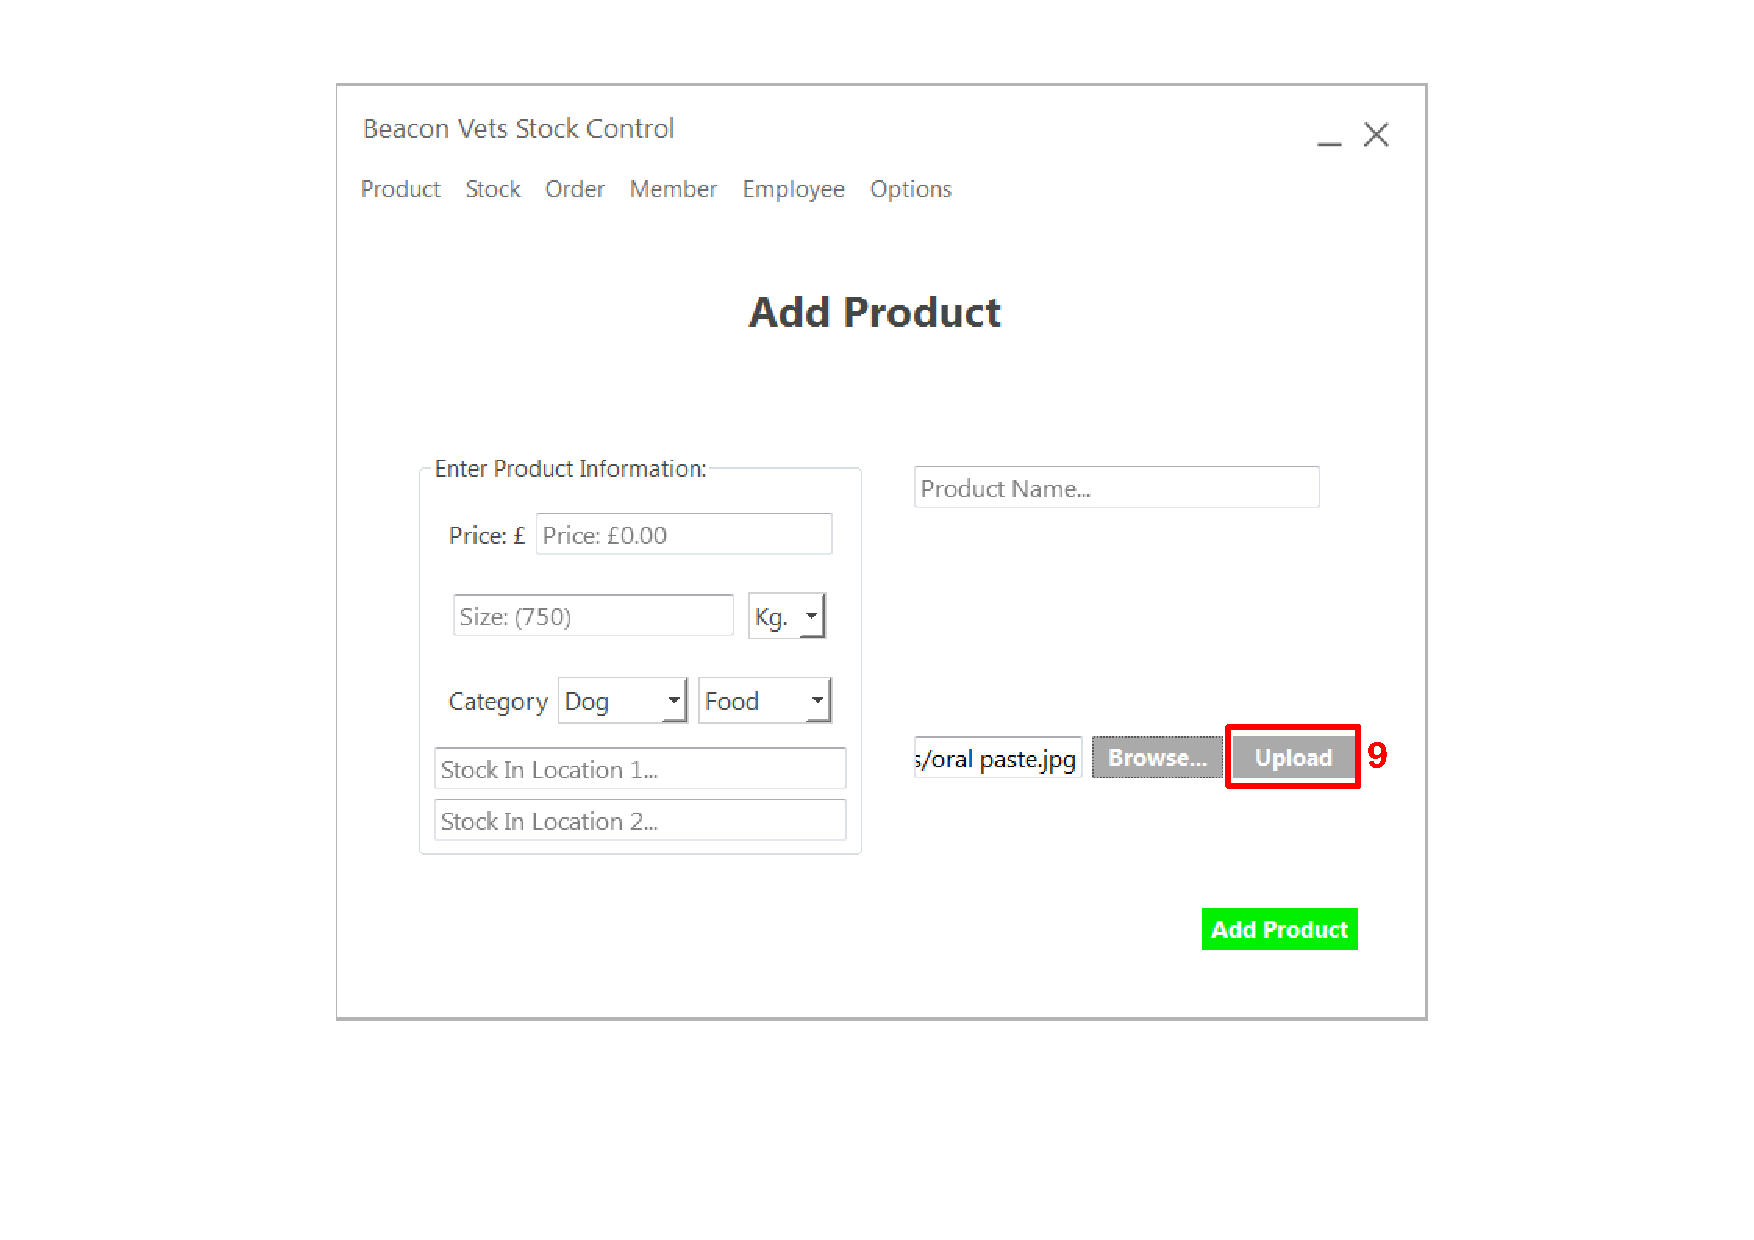
\includegraphics[width=8cm]{./ManualImages/add-product-8.pdf}

\textbf{10.} Click the `Add Product' button.

\includegraphics[width=8cm]{./ManualImages/add-product-9.pdf}

\textbf{11.} Click the `Yes' button in the pop up window.

\includegraphics[width=8cm]{./ManualImages/add-product-10.pdf}

\textbf{12.} Click the `Ok' button in the pop up window.

\includegraphics[width=8cm]{./ManualImages/add-product-11.pdf}

You have now successfully added a product to the database.

\pagebreak
\subsubsection{Adding a Member to the system}
\label{fig:Adding a Member to the system}

\textbf{1.} On any interface, click on the `Member' option in the menu-bar.

\includegraphics[width=8cm]{./ManualImages/add-member-1.pdf}

\textbf{2.} On the drop down menu, click on the `Add New Member' option.

\includegraphics[width=8cm]{./ManualImages/add-member-2.pdf}

An alternative to step 1 and step 2, is by pressing the `CTRL' and `M' button on the keyboard simultaneously.

\includegraphics[width=\textwidth]{./ManualImages/shortcut-member.pdf}

\textbf{3.} enter appropriate data into the data fields

\includegraphics[width=8cm]{./ManualImages/add-member-3.pdf}

\textbf{4.} choose an appropriate option from the drop down menus

\includegraphics[width=8cm]{./ManualImages/add-member-4.pdf}

if the postcode entered is located within Cumbria, go to step 5, otherwise, go to step 7 .

\textbf{5.} check the tick-box, a button will appear.

\includegraphics[width=8cm]{./ManualImages/add-member-5.pdf}

\textbf{6.} click the find button once a postcode has been entered, this should cause some of the data fields to be automatically completed.

\includegraphics[width=8cm]{./ManualImages/add-member-6.pdf}

\textbf{7.} click the `Add Member' button.

\includegraphics[width=8cm]{./ManualImages/add-member-7.pdf}

\textbf{8.} Click on the `Yes' button on the pop up window

\includegraphics[width=8cm]{./ManualImages/add-member-8.pdf}

\textbf{9.} Click on the `Ok' button on the pop up window

\includegraphics[width=8cm]{./ManualImages/add-member-9.pdf}

You have now successfully added a Member to the system.

\pagebreak
\subsubsection{Adding an Employee to the system}
\label{fig:Adding an Employee to the system}

\textbf{1.} On any interface, click on the `Employee' option within the menu bar.

\textbf{2.} Click on the `Add an Employee' option from the drop down menu.

\includegraphics[width=8cm]{./ManualImages/add-employee-1.pdf}

An alternative to step 1 and step 2, is by pressing the `CTRL' and `E' button on the keyboard simultaneously.

\includegraphics[width=\textwidth]{./ManualImages/shortcut-employee.pdf}

\pagebreak
\subsubsection{Editing a Product in the system}
\label{fig:Editing a Product in the system}

\textbf{1.} On any interface, click on the Product option in the menu bar.

\textbf{2.} Click on 'Edit a Product' in the dropdown menu.

\includegraphics[width=\textwidth]{./ManualImages/edit-product-1.pdf}

\textbf{3.} Enter the ProductID into the ProductID field. 

\textbf{4.} Press the 'Find' button.

\includegraphics[width=\textwidth]{./ManualImages/edit-product-2.pdf}

if you do not know the ProductID of the product you want to edit, find it using the Search window. For a tutorial on using the search window, go to page: . 

\textbf{5.} Edit the data for the product.

Note that the stock cannot be changed at this interface, for a tutorial on how to change the stock, go to page .

\textbf{6.} Click the 'Edit Product' button.

\includegraphics[width=\textwidth]{./ManualImages/edit-product-3.pdf}

\textbf{7.} Click the 'Yes' button.

\includegraphics[width=\textwidth]{./ManualImages/edit-product-4.pdf}

\textbf{8.} Click the 'Ok' button.

\includegraphics[width=\textwidth]{./ManualImages/edit-product-5.pdf}

You have now successfully edited a product.


\pagebreak
\subsubsection{Editing a Member currently in the system}
\label{fig:Editing a Member currently in the system}

\textbf{1.} On any interface, click on the Member button in the Menu bar.

\textbf{2.} In the drop down menu, click on the 'Edit a Member' button.

\includegraphics[width=\textwidth]{./ManualImages/edit-member-1.pdf}

\textbf{3.} Enter the MemberID into the MemberID field. 

\textbf{4.} Press the 'Find' button.

\includegraphics[width=\textwidth]{./ManualImages/edit-member-2.pdf}

if you do not know the MemberID of the member you want to edit, find it using the Search window. For a tutorial on using the search window, go to page: . 

\textbf{5.} Make the changes to the member information.

\textbf{6.}  Click the 'Edit Member' button.

\includegraphics[width=\textwidth]{./ManualImages/edit-member-3.pdf}

\textbf{7.}  Click the 'Yes' button.

\includegraphics[width=\textwidth]{./ManualImages/edit-member-4.pdf}

\textbf{8.} Click the 'Ok' button.

\includegraphics[width=\textwidth]{./ManualImages/edit-member-5.pdf}

You have now successfully edited a member.

\pagebreak
\subsubsection{Editing an Employee in the system}
\label{fig:Editing an Employee in the system}

\textbf{1.} On any interface, click on the employee button in the Menu bar.

\textbf{2.} From the drop down menu, click on the 'Edit an Employee' button.

If you cannot click on the 'Edit Employee' button, because the system will not let you, it is because you must be signed into the administrator account in order to edit an employee.

\includegraphics[width=\textwidth]{./ManualImages/edit-employee-1.pdf}

\textbf{3.} Enter the EmployeeID into the EmployeeID field.

\textbf{4.} Click on the 'Find' button.

\includegraphics[width=\textwidth]{./ManualImages/edit-employee-2.pdf}

\textbf{5.} enter the new data into the data fields.

\pagebreak
\subsubsection{Removing a Product from the system}
\label{fig:Removing a Product from the system}

\textbf{1.} On any interface, click on the Product option in the Menu bar

\textbf{2.} Click on `Delete a Product' from the drop down menu

\includegraphics[width=\textwidth]{./ManualImages/delete-product-1.pdf}

\textbf{3.} Enter the ProductID into the ProductID field.

\textbf{4.} Click the find button.

\includegraphics[width=\textwidth]{./ManualImages/delete-product-2.pdf}

The information about the product should be displayed.

\textbf{5.} Click on the `Delete Product' button in the bottom right hand corner of the program.

\includegraphics[width=\textwidth]{./ManualImages/delete-product-3.pdf}

\textbf{6.} Click the `Yes' button on the pop up window.

\textbf{7.} Click the `Ok' button on the second pop up window.

\includegraphics[width=\textwidth]{./ManualImages/delete-product-4.pdf}

you have now successfully deleted a product from the database.

\pagebreak
\subsubsection{Removing a Member from the system}
\label{fig:Removing a Member from the system}

\textbf{1.} On any interface, click on the Member option in the menu bar.

\textbf{2.} Click on the 'Delete a Member' button in the dropdown menu.

\includegraphics[width=\textwidth]{./ManualImages/delete-member-1.pdf}

\pagebreak

\textbf{3.} Enter the MemberID into the MemberID field.

\textbf{4.} Click on the 'Find' button once the MemberID has been entered.

\includegraphics[width=\textwidth]{./ManualImages/delete-member-2.pdf}

The information about the member should be displayed. you cannot edit this information.

\textbf{5.} Click on the Delete Member button in the bottom right hand corner of the system. 

\includegraphics[width=\textwidth]{./ManualImages/delete-member-3.pdf}

\textbf{6.} Click the 'Yes' button on the pop up window.

\textbf{7.} Click the 'Ok' button on the op up window.

\includegraphics[width=\textwidth]{./ManualImages/delete-member-4.pdf}

You have now successfully removed the member from the system.

\pagebreak
\subsubsection{Removing an Employee for the system.}
\label{fig:Removing an Employee for the system.}

\textbf{1.} On any interface, click on the Employee option in the menu bar.

\textbf{2.} Click on the 'Delete Employee' button in the drop down menu.

\includegraphics[width=\textwidth]{./ManualImages/delete-employee-1.pdf}

\textbf{3.} Enter the EmployeeID of the Employee into the EmployeeID field.

if you do not know a specific employee's EmployeeID, you can use the search window to find it. For a tutorial on using the search window, go to page \pageref{fig:Using the search window} of the User Manual.

\textbf{4.} click on the 'Find' button.

\includegraphics[width=\textwidth]{./ManualImages/delete-employee-2.pdf}

The employee information should be displayed. You will not be able to edit any of the information displayed here. For a tutorial on how to edit the employee information, go to page \pageref{fig:Editing an Employee in the system} of the User Manual.

\textbf{5.} Click on the 'Delete Employee' button in the bottom right hand corner of the system.

\includegraphics[width=\textwidth]{./ManualImages/delete-employee-3.pdf}

\textbf{6.} Click the 'Yes' button in the pop up window. This is cause another pop up window to open.

\textbf{7.}Click the 'Ok' button in the second pop up window and both the pop up windows will close. You have successfully removed the employee from the system.

\includegraphics[width=\textwidth]{./ManualImages/delete-employee-4.pdf}

\pagebreak
\subsubsection{Changing the stock of a Product}
\label{fig:Changing the stock of a Product}

\textbf{1.} To change the stock of a product you must be logged into the system.

\textbf{2.} Once logged in, click on the Stock option in the menu bar.

\textbf{3.} Now click on the Manage Stock option from the drop down menu. This is the only option in the menu.

\includegraphics[width=\textwidth]{./ManualImages/edit-stock-1.pdf}

\textbf{4.} Enter the ProductID of the product you want to change the stock for. If you do not know the ProductID of the product, you can find it using the search window. For a tutorial on using the search window, go to page \pageref{fig:Using the search window} of the User Manual.

\textbf{5.} Click on the find button after you have entered the ProductID.

\includegraphics[width=\textwidth]{./ManualImages/edit-stock-2.pdf}

\textbf{6.} Click the up or down arrows on the spin box to change the stock or enter the number into the field.

\includegraphics[width=\textwidth]{./ManualImages/edit-stock-3.pdf}

\textbf{7.} once you have changed the stock of the product, click on the 'Save' button in the bottom right hand corner of the system.

\includegraphics[width=\textwidth]{./ManualImages/edit-stock-4.pdf}

\textbf{8.} On the pop up window, click the 'Ok' button.

\includegraphics[width=\textwidth]{./ManualImages/edit-stock-5.pdf}

You have now successfully changed the stock of the product.


\pagebreak
\subsubsection{Product Stock Prediction}
\label{fig:Product Stock Prediction}

\textbf{1.} To get to the product stock prediction, follow steps 1 to 5 in the 'Changing the stock of a Product' section on page \pageref{fig:Changing the stock of a Product} of the User Manual.

In the 'Stock Prediction' section, There is a graph that displays the sales of the product. If there are no lines plotted on the graph, there have not been any sales of the product.

To the right of the graph there is a label that says "Predicted Sales Next Week". To the right of this should be a number which will represent the predicted sales of that product next week.

An unrealistic value of the stock prediction is usually due to lack of sales data in the graph. A more accurate predicted sales can be made by changing the graph to display the sales per day. To do this follow the following steps:

\textbf{2.} locate the drop down menu to the right of the 'View Sales per' text.

\includegraphics[width=\textwidth]{./ManualImages/change-stock-1.pdf}

\textbf{3.} Left click on the drop down menu and there should be two options, 'Day' and 'Week'

\includegraphics[width=\textwidth]{./ManualImages/change-stock-2.pdf}

\textbf{4.} To view the sales per week, click on the 'Week' button.

\textbf{5.} To view the sales per day, click on the 'Day' button.

\pagebreak
\subsubsection{Adding products to an order}
\label{fig:Adding products to an order}

\textbf{1.} Navigate to the `Create Order' interface. This can be done by clicking on `Order' in the menu bar, then click on `Create New Order' from the drop down menu.

\includegraphics[width=\textwidth]{./ManualImages/product-order-1.pdf}

\textbf{2.} Left click on a product in the `Find Product' table. This will cause it to be highlighted in green.

\includegraphics[width=\textwidth]{./ManualImages/product-order-2.pdf}

\textbf{3.} Click on the `Add to Order' button, ensuring the product is still selected.

\includegraphics[width=\textwidth]{./ManualImages/product-order-3.pdf}

The product should now appear in the `Current Order' table.

\includegraphics[width=\textwidth]{./ManualImages/product-order-4.pdf}

You have now successfully added a product to the order.

An alternative method to adding a product to the order, is by double left clicking on the product in the `Finding Product' table.

\pagebreak
\subsubsection{Applying a Discount to an Order}
\label{fig:Applying a Discount to an Order}

\textbf{1.} To apply a discount to the order, you must enter a MemberID into the MemberID field.

\includegraphics[width=\textwidth]{./ManualImages/discount-1.pdf}

\textbf{2.} Once you have entered the MemberID, click the `Enter' button

\includegraphics[width=\textwidth]{./ManualImages/discount-2.pdf}

\pagebreak

if the MemberID is valid when the `Enter' button is pressed, a 10 percent discount should be applied.

\includegraphics[width=\textwidth]{./ManualImages/discount-3.pdf}

\pagebreak
\subsubsection{Previewing the invoice}
\label{fig:Previewing the invoice}

\textbf{1.} Once you have created an invoice and would like to preview it, click on the `Preview' button.

\includegraphics[width=\textwidth]{./ManualImages/preview-1.pdf}

\pagebreak
\subsubsection{Printing an invoice}
\label{fig:Printing an invoice}

\textbf{1.} To print an invoice, you must first create one. Go to page \pageref{fig:Adding products to an order} for a tutorial on adding products to an order.

\textbf{2.} Once you have created the invoice you must click the check box named `Print Invoice'.

\includegraphics[width=\textwidth]{./ManualImages/print-1.pdf}

\pagebreak

\textbf{3.} Click the `Save' button.

\includegraphics[width=\textwidth]{./ManualImages/print-2.pdf}

\pagebreak

\textbf{4.} Before the invoice is saved, it will present you with the window below. Here you can select the printer and printer options to print the invoice.

\includegraphics[width=\textwidth]{./ManualImages/print-3.pdf}

\pagebreak

\textbf{5.} Once you have chosen the correct printer, click the `Print' button. This will then begin to print off the invoice.

\includegraphics[width=\textwidth]{./ManualImages/print-4.pdf}

\pagebreak
\subsubsection{Emailing an invoice}
\label{fig:Emailing an invoice}

\textbf{1.} To send the invoice via email, click the `Send Invoice to Email' check box.

\includegraphics[width=\textwidth]{./ManualImages/email-1.pdf}

\textbf{2.} You must next enter an email address to send the invoice to. This needs to be entered in the email address field highlighted below.

\includegraphics[width=\textwidth]{./ManualImages/email-2.pdf}

\pagebreak

\textbf{3.} Click the `Save' button.

\includegraphics[width=\textwidth]{./ManualImages/print-2.pdf}

\textbf{4.} Once the pop up window below displays, the system will have successfully sent the invoice to the email entered and saved the invoice.

\includegraphics[width=\textwidth]{./ManualImages/email-3.pdf}

\pagebreak
\subsubsection{Changing information on the invoice}
\label{fig:Changing information on the invoice}

The information highlighted in the invoice below can be changed in the preferences interface.

\includegraphics[width=\textwidth]{./ManualImages/change-info-1.pdf}

\pagebreak

\textbf{1.} Click on `Options' in the menu bar.

\textbf{2.} Click on `Preferences' from the drop down menu.

\includegraphics[width=\textwidth]{./ManualImages/change-info-2.pdf}

\pagebreak

\textbf{3.} Change the information under the `Company Info' section. The data fields have been highlighted in the screen shot below.

\includegraphics[width=\textwidth]{./ManualImages/change-info-3.pdf}

For a tutorial on changing the logo, see Step 6-9 of the Adding Product tutorial on page \pageref{fig:Adding a Product to the system}

\pagebreak

\textbf{4.} Once you have changed the company details, click on the `Save' button in the bottom right hand corner of the Preferences interface.

\includegraphics[width=\textwidth]{./ManualImages/change-info-4.pdf}

\pagebreak

\textbf{5.} You have now saved the preferences. Click the `Ok' button on the pop up window to close it.

\includegraphics[width=\textwidth]{./ManualImages/change-info-5.pdf}

\pagebreak
\subsubsection{Accessing the search window}
\label{fig:Accessing the search window}

\textbf{1.} Click on the `Options' button in the menu bar.

\textbf{2.} Click on the `Search Window' option in the drop down menu.

\includegraphics[width=\textwidth]{./ManualImages/access-search-1.pdf}

\pagebreak

\textbf{3.} You have successfully opened the search window. To close the search window, click on the `X' in the top right hand corner of the window.

\includegraphics[width=\textwidth]{./ManualImages/access-search-2.pdf}

For a tutorial on how to use the Search window, go to page \pageref{fig:Using the search window} of the user manual.


\pagebreak
\subsubsection{Using the search window}
\label{fig:Using the search window}

\textbf{1.} Open the search window. For a tutorial on how to open the search window, go to page \pageref{fig:Accessing the search window} of the user manual.

A short-cut for opening the Search window is by pressing the `CTRL' and `F' buttons on the keyboard simultaneously.

\includegraphics[width=\textwidth]{./ManualImages/shortcut-search.pdf}

\textbf{2.} To find a specific product within the system, enter a keyword into the search field.

\includegraphics[width=\textwidth]{./ManualImages/search-1.pdf}

\textbf{3.} By Default, the search window searches for products. To search for a member or an employee, follow steps 4- .

\textbf{4.} To change the table that is displayed and to search for either a product, member or employee, left click on the text that says `Product'.

\includegraphics[width=\textwidth]{./ManualImages/search-2.pdf}

\textbf{5.} A drop down menu will be displayed, select the option you want to search for (product, member or employee).

\includegraphics[width=\textwidth]{./ManualImages/search-3.pdf}

\textbf{6.} Click a column heading to sort the results from A-Z, Z-A, 1-9, 9-1, ect...

\includegraphics[width=\textwidth]{./ManualImages/search-4.pdf}

\textbf{7.} Right click on an item within the table. A drop down menu will be displayed. The drop down menu that is displayed, depends on what you are searching for, whether it be a product, member or an employee.

\includegraphics[width=\textwidth]{./ManualImages/search-5.pdf}

\textbf{8.} Clicking on one of the options in the drop down menu will take you to the associated interface. For example clicking on edit product will take you to the edit product interface.


\subsection{Saving}

All the saving in the system is done internally and is automatically handled by the system. The system automatically saves the database file after each query that is executed within the database. This helps prevent any data loss in the event of the system crashing.

\subsection{Limitations}

The only feature specified in my analysis and design that was not implemented into the final program was that an image of the product is not displayed in the search window. This does not cause any problems in the system, other than products can not be located based on what they look like.

\section{Error Recovery}

\subsection{Sorry the Username and Password are incorrect.}

This error will occur when trying to log into the system and the username and password in which you have entered do not match any of the accounts stored in the system.

To resolve this problem, you can try to re-enter your username and password, to ensure that you have entered the correct details. If the problem still persists, then go to page \pageref{fig:Forgetting Your User-name or Password} of the user manual, for a tutorial on how to retrieve your account details.

\subsection{The Gmail Account Details are not valid.}

This error is caused when trying to send an email from the system. The error occurs because the email address and password used to send the email from is not valid.

To change the email and password, click on the 'Options' button in the menu bar and then click on 'Preferences' from the drop down menu.

Under the 'Email Account' section, you will find an email and password field. By default, the email address and password are 'example@gmail.com' and 'password'.

Change the email address and password to ones of a working gmail account. Please note that it will only work with an '@gmail.com' account.

Once the email address and password have been changed, click on the 'Save button in the bottom right hand corner of the Preferences interface. This will now save the new email address and password to the system. If the new email address and password are valid, the error message should no longer be displayed and the system should successfully send the email.

\subsection{Sorry the Email address does not match any of the Accounts.}

This error will occur when trying to reset your password. It occurs because the email address in which you have entered does not match any of the email addresses associated to the employee accounts within the system.

To resolve this issue, ensure that the email address you have entered is spelt correctly and if the problem still persists, another user can sign into the system and use the search window to find the email address associated to your account. For a more detailed explanation on how to do this, go to page \pageref{fig:Using the search window} of the user manual.

\subsection{No Product with ProductID:}

This error occurs on either the edit or delete product interface. This issue is caused when the user enters the ProductID of a product that is not in the database.This issue is resolved simply by entering the ProductID of a valid product. The search window can be used to find the ProductID of each product. if you require assistance on using the search window, go to page \pageref{fig:Accessing the search window} of the user manual for a tutorial on how to open the search window, or go to page \pageref{fig:Using the search window} of the user manual, for tutorial on how to use the search window.

\subsection{No User found with MemberID:}

This error occurs on either the edit or delete member interface. This issue is caused when the user enters the MemberID of a member that is not in the database.This issue is resolved simply by entering the MemberID of a valid member. The search window can be used to find the MemberID of each member. if you require assistance on using the search window, go to page \pageref{fig:Accessing the search window} of the user manual for a tutorial on how to open the search window, or go to page \pageref{fig:Using the search window} of the user manual, for tutorial on how to use the search window.

\subsection{No employee found with EmployeeID:}

This error occurs on either the edit or delete employee interface. This issue is caused when the user enteres the EmployeeID of an employee that is not in the database.This issue is resolved simply by entering the EmployeeID of a valid employee. The search window can be used to find the EmployeeID of each employee. if you require assistance on using the search window, go to page \pageref{fig:Accessing the search window} of the user manual, for a tutorial on how to open the search window, or go to page \pageref{fig:Using the search window} of the user manual, for tutorial on how to use the search window.



\section{System Recovery}

\subsection{Backing-up Data}

\textbf{1.} Go to the `Stock Control System' folder created during the System Installation section.

\includegraphics[width=\textwidth]{./ManualImages/recovery-1.pdf}

\textbf{2.} Double click on the folder and locate the `ProductDatabase.db file.

\includegraphics[width=\textwidth]{./ManualImages/recovery-2.pdf}

\textbf{3.} Right click on the file and click on `Copy' from the drop down menu.

\includegraphics[width=\textwidth]{./ManualImages/recovery-3.pdf}

\textbf{4.} Move the copy of the `ProductDatabse.db' file onto a removable storage media device such as a USB flash drive or an external hard drive.

\includegraphics[width=\textwidth]{./ManualImages/recovery-4.pdf}

You have now successfully backed up the database. Remove the removable medis storage device and store in a secure and memorable place. Go to page \pageref{fig:Restoring Data} of the user manual, for a tutorial on how to restore the data from a back-up.

\pagebreak
\subsection{Restoring Data}
\label{fig:Restoring Data}

\textbf{1.} connect the removable media storage to the computer.

\includegraphics[width=\textwidth]{./ManualImages/back-up-1.pdf}

\textbf{2.} Locate the `ProductDatabase.db' file on the removable media storage device.

\includegraphics[width=\textwidth]{./ManualImages/back-up-2.pdf}

\pagebreak

\textbf{3.} Delete the `ProductDatabase.db' file currently in the Stock Control System folder.

\textbf{4.} Drag and drop the `ProductDatabase.db' file from the removable media storage device into the `Stock Control System' folder.

\includegraphics[width=\textwidth]{./ManualImages/back-up-3.pdf}

\textbf{5.} Run the system and the database from the back up should now be working with the system.

\stopcontents[chapters]